%==============================================================================
% Tento soubor použijte jako základ
% This file should be used as a base for the thesis
% Autoři / Authors: 2008 Michal Bidlo, 2022 Jaroslav Dytrych
% Kontakt pro dotazy a připomínky: sablona@fit.vutbr.cz
% Contact for questions and comments: sablona@fit.vutbr.cz
%==============================================================================
% kódování: UTF-8 (zmena prikazem iconv, recode nebo cstocs)
% encoding: UTF-8 (you can change it by command iconv, recode or cstocs)
%------------------------------------------------------------------------------
% zpracování / processing: make, make pdf, make clean
%==============================================================================
% Soubory, které je nutné upravit nebo smazat: / Files which have to be edited or deleted:
%   projekt-20-literatura-bibliography.bib - literatura / bibliography
%   projekt-01-kapitoly-chapters.tex - obsah práce / the thesis content
%   projekt-01-kapitoly-chapters-en.tex - obsah práce v angličtině / the thesis content in English
%   projekt-30-prilohy-appendices.tex - přílohy / appendices
%   projekt-30-prilohy-appendices-en.tex - přílohy v angličtině / appendices in English
%==============================================================================
%\documentclass[]{fitthesis} % bez zadání - pro začátek práce, aby nebyl problém s překladem
%\documentclass[english]{fitthesis} % without assignment - for the work start to avoid compilation problem
%\documentclass[zadani]{fitthesis} % odevzdani do IS VUT a/nebo tisk s barevnými odkazy - odkazy jsou barevné
%\documentclass[english,zadani]{fitthesis} % for submission to the IS VUT and/or print with color links - links are color
%\documentclass[zadani,print]{fitthesis} % pro černobílý tisk - odkazy jsou černé
%\documentclass[english,zadani,print]{fitthesis} % for the black and white print - links are black
%\documentclass[zadani,cprint]{fitthesis} % pro barevný tisk - odkazy jsou černé, znak VUT barevný
\documentclass[english,zadani,cprint]{fitthesis} % for the print - links are black, logo is color
% * Je-li práce psaná v anglickém jazyce, je zapotřebí u třídy použít 
%   parametr english následovně:
%   If thesis is written in English, it is necessary to use 
%   parameter english as follows:
%      \documentclass[english]{fitthesis}
% * Je-li práce psaná ve slovenském jazyce, je zapotřebí u třídy použít 
%   parametr slovak následovně:
%   If the work is written in the Slovak language, it is necessary 
%   to use parameter slovak as follows:
%      \documentclass[slovak]{fitthesis}
% * Je-li práce psaná v anglickém jazyce se slovenským abstraktem apod., 
%   je zapotřebí u třídy použít parametry english a enslovak následovně:
%   If the work is written in English with the Slovak abstract, etc., 
%   it is necessary to use parameters english and enslovak as follows:
%      \documentclass[english,enslovak]{fitthesis}

% Základní balíčky jsou dole v souboru šablony fitthesis.cls
% Basic packages are at the bottom of template file fitthesis.cls
% zde můžeme vložit vlastní balíčky / you can place own packages here


% Pro seznam zkratek lze využít balíček Glossaries - nutno odkomentovat i níže a při kompilaci z konzoly i v Makefile (plnou verzi pro Perl, nebo lite)
% The Glossaries package can be used for the list of abbreviations - it is necessary to uncomment also below. When compiling from the console also in the Makefile (full version for Perl or lite)
%\usepackage{glossaries}
%\usepackage{glossary-superragged}
%\makeglossaries 

% Nastavení cesty k obrázkům
% Setting of a path to the pictures
\graphicspath{{obrazky-figures/}{./obrazky-figures/}}
%\graphicspath{{obrazky-figures/}{../obrazky-figures/}}

%---rm---------------
\renewcommand{\rmdefault}{lmr}%zavede Latin Modern Roman jako rm / set Latin Modern Roman as rm
%---sf---------------
\renewcommand{\sfdefault}{qhv}%zavede TeX Gyre Heros jako sf
%---tt------------
\renewcommand{\ttdefault}{lmtt}% zavede Latin Modern tt jako tt

% vypne funkci šablony, která automaticky nahrazuje uvozovky,
% aby nebyly prováděny nevhodné náhrady v popisech API apod.
% disables function of the template which replaces quotation marks
% to avoid unnecessary replacements in the API descriptions etc.
\csdoublequotesoff

\usepackage{url}

% =======================================================================
% balíček "hyperref" vytváří klikací odkazy v pdf, pokud tedy použijeme pdflatex
% problém je, že balíček hyperref musí být uveden jako poslední, takže nemůže
% být v šabloně
% "hyperref" package create clickable links in pdf if you are using pdflatex.
% Problem is that this package have to be introduced as the last one so it 
% can not be placed in the template file.
\ifWis
\ifx\pdfoutput\undefined % nejedeme pod pdflatexem / we are not using pdflatex
\else
  \usepackage{color}
  \usepackage[unicode,colorlinks,hyperindex,plainpages=false,pdftex]{hyperref}
  \definecolor{hrcolor-ref}{RGB}{223,52,30}
  \definecolor{hrcolor-cite}{HTML}{2F8F00}
  \definecolor{hrcolor-urls}{HTML}{092EAB}
  \hypersetup{
	linkcolor=hrcolor-ref,
	citecolor=hrcolor-cite,
	filecolor=magenta,
	urlcolor=hrcolor-urls
  }
  \def\pdfBorderAttrs{/Border [0 0 0] }  % bez okrajů kolem odkazů / without margins around links
  \pdfcompresslevel=9
\fi
\else % pro tisk budou odkazy, na které se dá klikat, černé / for the print clickable links will be black
\ifx\pdfoutput\undefined % nejedeme pod pdflatexem / we are not using pdflatex
\else
  \usepackage{color}
  \usepackage[unicode,colorlinks,hyperindex,plainpages=false,pdftex,urlcolor=black,linkcolor=black,citecolor=black]{hyperref}
  \definecolor{links}{rgb}{0,0,0}
  \definecolor{anchors}{rgb}{0,0,0}
  \def\AnchorColor{anchors}
  \def\LinkColor{links}
  \def\pdfBorderAttrs{/Border [0 0 0] } % bez okrajů kolem odkazů / without margins around links
  \pdfcompresslevel=9
\fi
\fi
% Řešení problému, kdy klikací odkazy na obrázky vedou za obrázek
% This solves the problems with links which leads after the picture
\usepackage[all]{hypcap}

\usepackage{subcaption}
\usepackage{pdfpages}

\lstdefinestyle{mystyle}{
    backgroundcolor=\color{white},   
    commentstyle=\color{olive},
    keywordstyle=\color{blue},
    numberstyle=\tiny\color{gray},
    stringstyle=\color{orange},
    basicstyle=\ttfamily\footnotesize,
    breakatwhitespace=false,         
    breaklines=true,                 
    captionpos=b,                    
    keepspaces=true,                 
    numbers=left,                    
    numbersep=5pt,                  
    showspaces=false,                
    showstringspaces=false,
    showtabs=false,                  
    tabsize=4,
    escapeinside={^}{^}
}

\lstset{style=mystyle}
% Informace o práci/projektu / Information about the thesis
%---------------------------------------------------------------------------
\projectinfo{
  %Prace / Thesis
  project={BP},            %typ práce BP/SP/DP/DR  / thesis type (SP = term project)
  year={2024},             % rok odevzdání / year of submission
  date=\today,             % datum odevzdání / submission date
  %Nazev prace / thesis title
  title.cs={Generování kódu z textového popisu funkcionality},  % název práce v češtině či slovenštině (dle zadání) / thesis title in czech language (according to assignment)
  title.en={Generating Code from Textual Description of Functionality}, % název práce v angličtině / thesis title in english
  %title.length={14.5cm}, % nastavení délky bloku s titulkem pro úpravu zalomení řádku (lze definovat zde nebo níže) / setting the length of a block with a thesis title for adjusting a line break (can be defined here or below)
  %sectitle.length={14.5cm}, % nastavení délky bloku s druhým titulkem pro úpravu zalomení řádku (lze definovat zde nebo níže) / setting the length of a block with a second thesis title for adjusting a line break (can be defined here or below)
  %dectitle.length={14.5cm}, % nastavení délky bloku s titulkem nad prohlášením pro úpravu zalomení řádku (lze definovat zde nebo níže) / setting the length of a block with a thesis title above declaration for adjusting a line break (can be defined here or below)
  %Autor / Author
  author.name={Ondřej},   % jméno autora / author name
  author.surname={Zobal},   % příjmení autora / author surname
  %author.title.p={Bc.}, % titul před jménem (nepovinné) / title before the name (optional)
  %author.title.a={Ph.D.}, % titul za jménem (nepovinné) / title after the name (optional)
  %Ustav / Department
  department={UPGM}, % doplňte příslušnou zkratku dle ústavu na zadání: UPSY/UIFS/UITS/UPGM / fill in appropriate abbreviation of the department according to assignment: UPSY/UIFS/UITS/UPGM
  % Školitel / supervisor
  supervisor.name={Pavel},   % jméno školitele / supervisor name
  supervisor.surname={Smrž},   % příjmení školitele / supervisor surname
  supervisor.title.p={doc. RNDr.},   %titul před jménem (nepovinné) / title before the name (optional)
  supervisor.title.a={Ph.D.},    %titul za jménem (nepovinné) / title after the name (optional)
  % Klíčová slova / keywords
  keywords.cs={strojové učení, zpracování přirozeného jazyka, ML, NLP, zlepšení kódu, generování komentářů, refaktorizace, Longformer, PLBART, Visual Studio Code, rozšíření}, % klíčová slova v českém či slovenském jazyce / keywords in czech or slovak language
  keywords.en={machine learning, natural language processing, ML, NLP, code refinement, comment generation, refactoring, Longformer, PLBART, Visual Studio Code, extension }, % klíčová slova v anglickém jazyce / keywords in english
  %keywords.en={Here, individual keywords separated by commas will be written in English.},
  % Abstrakt / Abstract
  abstract.cs={Tato práce se zabývá vývojem rozšíření do editoru Visual Studio Code, které pomůže vývojářům udržet kvalitu kódu jazyka Python 3. Rozšíření poskytuje možnost generování komentářů a docstringů, návrhu nových jmen proměnných. Rozšíření využívá velké jazykové modely Transformer s řídkou pozorností pro zpracování výsledků. Výsledky bohužel nekonkurují současné konkurenci, jakou je například GPT-3.5-turbo.}, % abstrakt v českém či slovenském jazyce / abstract in czech or slovak language
  abstract.en={This thesis is concerned with the development of an extension for the Visual Studio Code editor that helps developers maintain code quality in Python 3 by generating comments and docstrings and suggesting new names for variables. The extension was also supposed to include a bug fixing system, but unfortunately it failed to become effective. The system uses large Transformer language models with sparse attention for processing results. Unfortunately, the results do not compete with current competition such as GPT-3.5-turbo.}, % abstrakt v anglickém jazyce / abstract in english
  %abstract.en={An abstract of the work in English will be written in this paragraph.},
  % Prohlášení (u anglicky psané práce anglicky, u slovensky psané práce slovensky; u projektové praxe lze zakomentovat) / Declaration (for thesis in english should be in english; for project practice can be commented out)
%   declaration={Prohlašuji, že jsem tuto bakalářskou práci vypracoval samostatně pod vedením pana X...
% Další informace mi poskytli...
% Uvedl jsem všechny literární prameny, publikace a další zdroje, ze kterých jsem čerpal.},
   declaration={I hereby declare that this Bachelor's thesis was prepared as an original work by the author under the supervision of doc.\,Pavel Smrž.
 %The supplementary information was provided by Mr. Y
 I have listed all the literary sources, publications and other sources, which were used during the preparation of this thesis.},
  % Poděkování (nepovinné, nejlépe v jazyce práce; nechcete-li, zakomentujte pro skrytí nadpisu) / Acknowledgement (optional, ideally in the language of the thesis; comment out for hiding including heading)
  acknowledgment={I extend my heartfelt thanks to doc.\,Pavel Smrž for his professional guidance, support, and patience through these past two semesters.},
  %acknowledgment={Here it is possible to express thanks to the supervisor and to the people which provided professional help
%(external submitter, consultant, etc.).},
  % Rozšířený abstrakt (cca 3 normostrany) - lze definovat zde nebo níže / Extended abstract (approximately 3 standard pages) - can be defined here or below
  %extendedabstract={Do tohoto odstavce bude zapsán rozšířený výtah (abstrakt) práce v českém (slovenském) jazyce.},
  %extabstract.odd={true}, % Začít rozšířený abstrakt na liché stránce? / Should extended abstract start on the odd page?
  %faculty={FIT}, % FIT/FEKT/FSI/FA/FCH/FP/FAST/FAVU/USI/DEF
  faculty.cs={Fakulta informačních technologií}, % Fakulta v češtině - pro využití této položky výše zvolte fakultu DEF / Faculty in Czech - for use of this entry select DEF above
  faculty.en={Faculty of Information Technology}, % Fakulta v angličtině - pro využití této položky výše zvolte fakultu DEF / Faculty in English - for use of this entry select DEF above
  %department.cs={Ústav matematiky}, % Ústav v češtině - pro využití této položky výše zvolte ústav DEF nebo jej zakomentujte / Department in Czech - for use of this entry select DEF above or comment it out
  %department.en={Institute of Mathematics} % Ústav v angličtině - pro využití této položky výše zvolte ústav DEF nebo jej zakomentujte / Department in English - for use of this entry select DEF above or comment it out
}

% Rozšířený abstrakt (cca 3 normostrany) - lze definovat zde nebo výše / Extended abstract (approximately 3 standard pages) - can be defined here or above
%\extendedabstract{Do tohoto odstavce bude zapsán výtah (abstrakt) práce v českém (slovenském) jazyce.}
% Začít rozšířený abstrakt na liché stránce? / Should extended abstract start on the odd page?
%\extabstractodd{true}

% nastavení délky bloku s titulkem pro úpravu zalomení řádku - lze definovat zde nebo výše / setting the length of a block with a thesis title for adjusting a line break - can be defined here or above
%\titlelength{14.5cm}
% nastavení délky bloku s druhým titulkem pro úpravu zalomení řádku - lze definovat zde nebo výše / setting the length of a block with a second thesis title for adjusting a line break - can be defined here or above
%\sectitlelength{14.5cm}
% nastavení délky bloku s titulkem nad prohlášením pro úpravu zalomení řádku - lze definovat zde nebo výše / setting the length of a block with a thesis title above declaration for adjusting a line break - can be defined here or above
%\dectitlelength{14.5cm}

% řeší první/poslední řádek odstavce na předchozí/následující stránce
% solves first/last row of the paragraph on the previous/next page
\clubpenalty=10000
\widowpenalty=10000

% checklist
\newlist{checklist}{itemize}{1}
\setlist[checklist]{label=$\square$}

% Kompilace po částech (rychlejší, ale v náhledu nemusí být vše aktuální)
% Compilation piecewise (faster, but not all parts in preview will be up-to-date)
% Další informace viz / For more information see https://www.overleaf.com/learn/latex/Multi-file_LaTeX_projects
% \usepackage{subfiles}

% Nechcete-li, aby se u oboustranného tisku roztahovaly mezery pro zaplnění stránky, odkomentujte následující řádek / If you do not want enlarged spacing for filling of the pages in case of duplex printing, uncomment the following line
% \raggedbottom

\begin{document}
  % Vysazeni titulnich stran / Typesetting of the title pages
  % ----------------------------------------------
  \maketitle
  % Obsah
  % ----------------------------------------------
  \setlength{\parskip}{0pt}

  {\hypersetup{hidelinks}\setcounter{tocdepth}{1}\tableofcontents}
  
  % Seznam obrazku a tabulek (pokud prace obsahuje velke mnozstvi obrazku, tak se to hodi)
  % List of figures and list of tables (if the thesis contains a lot of pictures, it is good)
  \ifczech
    \renewcommand\listfigurename{Seznam obrázků}
  \fi
  \ifslovak
    \renewcommand\listfigurename{Zoznam obrázkov}
  \fi
  {\hypersetup{hidelinks}\listoffigures}
  
  \ifczech
    \renewcommand\listtablename{Seznam tabulek}
  \fi
  \ifslovak
    \renewcommand\listtablename{Zoznam tabuliek}
  \fi
  % {\hypersetup{hidelinks}\listoftables}

  % Seznam zkratek / List of abbreviations
  %\ifczech
  %  \renewcommand*\glossaryname{Seznam zkratek}%
  %  \renewcommand*\entryname{Zkratka}
  %  \renewcommand*\descriptionname{Význam}
  %\fi
  %\ifslovak
  %  \renewcommand*\glossaryname{Zoznam skratiek}%
  %  \renewcommand*\entryname{Skratka}
  %  \renewcommand*\descriptionname{Význam}
  %\fi
  %\ifenglish
  %  \renewcommand*\glossaryname{List of abbreviations}%
  %  \renewcommand*\entryname{Abbreviation}
  %  \renewcommand*\descriptionname{Meaning}
  %\fi
  % Definice zkratek - z textu se odkazují např. \Gls{TF–IDF}
  % Definition of abbreviations - referred from the text e.g. \Gls{TF–IDF}
  %\newglossaryentry{TF–IDF}
  %{
  %  name={TF–IDF},
  %  description={Term Frequency-Inverse Document Frequency}
  %}
  % 
  %\setglossarystyle{superragged}
  %\printglossaries

  \ifODSAZ
    \setlength{\parskip}{0.5\bigskipamount}
  \else
    \setlength{\parskip}{0pt}
  \fi

  % vynechani stranky v oboustrannem rezimu
  % Skip the page in the two-sided mode
  \iftwoside
    \cleardoublepage
  \fi

  % Text prace / Thesis text
  % ----------------------------------------------
  \ifenglish
    % This file should be replaced with your file with thesis content.
%=========================================================================
% Authors: Michal Bidlo, Bohuslav Křena, Jaroslav Dytrych, Petr Veigend and Adam Herout 2019, Ondřej Zobal 2024

% For compilation piecewise (see projekt.tex), it is necessary to uncomment it and change
% \documentclass[../projekt.tex]{subfiles}
% \begin{document}

%% ###                            
%%  #  #    # ##### #####   ####  
%%  #  ##   #   #   #    # #    # 
%%  #  # #  #   #   #    # #    # 
%%  #  #  # #   #   #####  #    # 
%%  #  #   ##   #   #   #  #    # 
%% ### #    #   #   #    #  ####  

\chapter{Introduction}

%% Context and Rationale
In the fast-paced field of software development, maintaining code quality and readability is crucial. This thesis introduces a tool for automatic code refactoring aid using Large Language Models (LLM), which aims to enhance code readability, quality, as well as the overall developer experience.  

Most contemporary tools lean heavily on chatting with generative AI assistants\footnote{Among those most popular by developers are copilot and chatGPT. Copilot offers next token prediction and chatting and is powered by GPT-3.5, chatGPT can only do chatting and is powered by GPT-3.5 and GPT-4}; these are usually very flexible, often able to perform operations they never directly saw in their training data; however, due to their broad focus, they often lack mastery.  Additionally, chatting doesn't make for the best workflow, especially when dealing with simple tasks that need to be performed often. Despite the recent language modeling boom, IDEs still lack more integrated AI tools for performing simple chores.

%% Specific Challenges Addressed
The aim of this thesis is to design, implement, and evaluate a \emph{VS Code/Code-OSS}\footnote{Code-OSS is a Free project developed by Microsoft, and Microsoft Visual Studio Code (VS Code for short) is its most popular distribution.} extension called \emph{CodeImprove} that uses AI to assist Python developers by enhancing code quality. Specifically, the extension will attempt to automate the generation of docstrings and comments, suggest more fitting variable names, and identify as well as fix common coding errors. 

%% Innovative Approach
To address these challenges while retraining reasonable hardware requirements, this thesis uses the Longformer. This sparse attention transformer model saves memory by focusing on a smaller window of code at a time. This paper also experiments with quantized low-rank adaptation, a different approach for reducing the memory use of large language models.

%% Structure of the Thesis
The thesis is organized as follows: An exploration of the theory behind contemporary state-of-the-art natural language processors is conducted over the next three chapters, ranging from neurons to the transformer model. The technologies employed in this project will be presented, along with the training data utilized for model creation, and are explained. Subsequently, the manner in which the models were trained is showcased, followed by details of the implementation of the extensions. Lastly, the evaluation of performance is examined, and the results are summarized.

%% ===================================================
%%  _   _                      _   _   _      _
%% | \ | | ___ _   _ _ __ __ _| | | \ | | ___| |_ ___
%% |  \I |/ _ \ | | | '__/ _` | | |  \I |/ _ \ __/ __|
%% | |\  |  __/ |_| | | | (_| | | | |\  |  __/ |_\__ \
%% |_| \_|\___|\__,_|_|  \__,_|_| |_| \_|\___|\__|___/
%% ===================================================

%%% LARGE LANGUAGE MODELS

\chapter{Neural networks}
\label{sec:neural_networks}

This chapter will go over the theory behind \emph{neural networks (NN)}, also sometimes called \emph{Artificial Neural Networks} (ANN), which are a cornerstone in machine learning. Neural networks enable computers to gain intuition in complex tasks by learning from vast amounts of data, relying solely on matrix multiplication and a handful of other simple mathematical functions for generating their predictions.

Neural networks are a branch of artificial intelligence. They are computational models designed to recognize patterns and solve complex problems. Neural networks can learn from datasets featuring examples of problems with solutions. Later chapters will explain how neural networks can be used to intelligently transform and generate textual content \ref{sec:llm}. Information in this chapter is based on\,\cite{DeepLearning2016}.

\medskip

Neural networks are a model that \emph{approximates} a given function $y = f^{*}(x)$ by defining a function $y = f(x,\theta)$ and learning the value $\theta$ so that the outputs of $f$ are as close as possible to the outputs of~$f^{*}$.

Neural networks can be represented as a composition of various functions within a directed graph. This chapter will focus on \emph{feedforward networks} that are an \emph{acyclic} variant of neural networks, meaning they do not contain feedback connections to previous layers. Some feedforward network $f(x)$ can be characterized as $f(x) = f_{n}(f_{2}(f_{1}(x)))$ as shown in \ref{fig:nn-functional}.

\begin{figure}[ht]
  \centering
  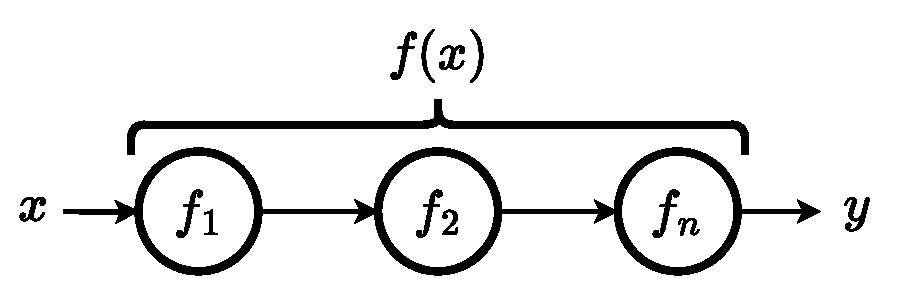
\includegraphics[width=0.55\textwidth]{neural-net-functional.pdf}
  \caption{$x$ is an input passed to the first layer $f_{1}$. Its output is passed to the second layer $f_{2}$ and so on until it arrives at $f_{n}$, which is the last layer, and its output is the output of the model.}
  \label{fig:nn-functional}
\end{figure}

Dataset defines \emph{inputs} and \emph{labels} representing $x$ and $f(x)$, respectively. In a neural network, inputs correspond to the value of the \emph{input layer} and labels to the desired value of the \emph{output layer}. Any other layers between them do not have their values bound by the dataset; because of this, they are called \emph{hidden layers}.

Inputs, labels, and outputs of individual layer functions are usually \emph{vector-valued}. The dimensionality of a layer is called \emph{width}. Each unit in these vectors can be visualized as a node that operates in parallel to other nodes within the same layer. These nodes are called \emph{neurons} for their functional similarity to their biological counterparts.

\medskip
The goal of using hidden layers is for the network to be able to split a potentially complex task into more manageable sub-tasks that can then be divided between the layers. However, by only using linear operations, the network's learning potential is limited to only observing linear relationships in the data. This can be solved by employing a \emph{non-linear function} to transform the output of our linear layer. This function is called an \emph{activation function}.

The activation function does not require its own trainable parameters, and the function itself does not need to be very complex. The most popular non-linear function is \emph{ReLU}, which consists of a constant function that changes into a linear function for $x > 0$ as pictured in figure \ref{fig:relu}.

The final output value of a neuron is called an \emph{activation}.

\begin{figure}[ht]
  \centering
  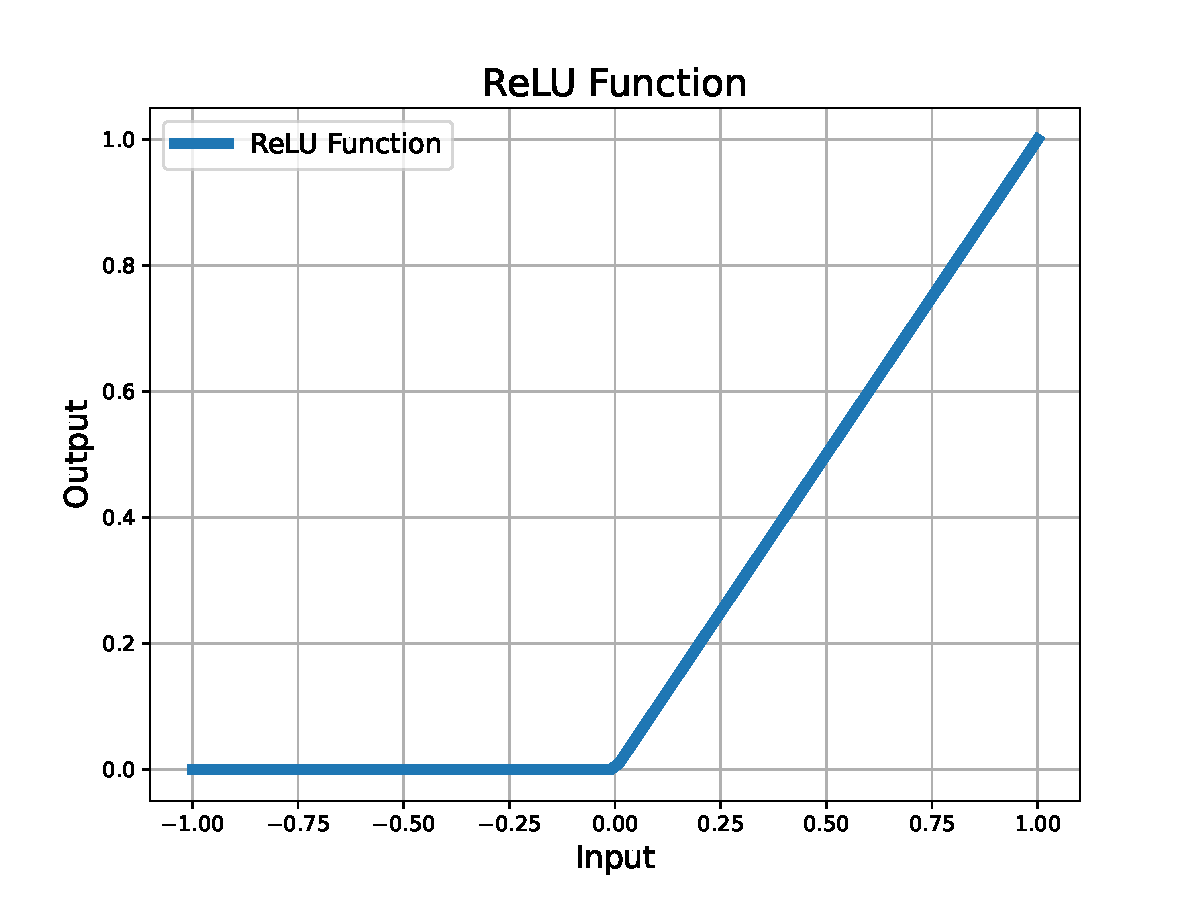
\includegraphics[width=0.7\textwidth]{relu.pdf}
  \caption{ReLU function graph. It is a primitive yet powerful activation function with great results with models that use a large number of layers.}
  \label{fig:relu}
\end{figure}

\begin{figure}[ht]
  \centering
  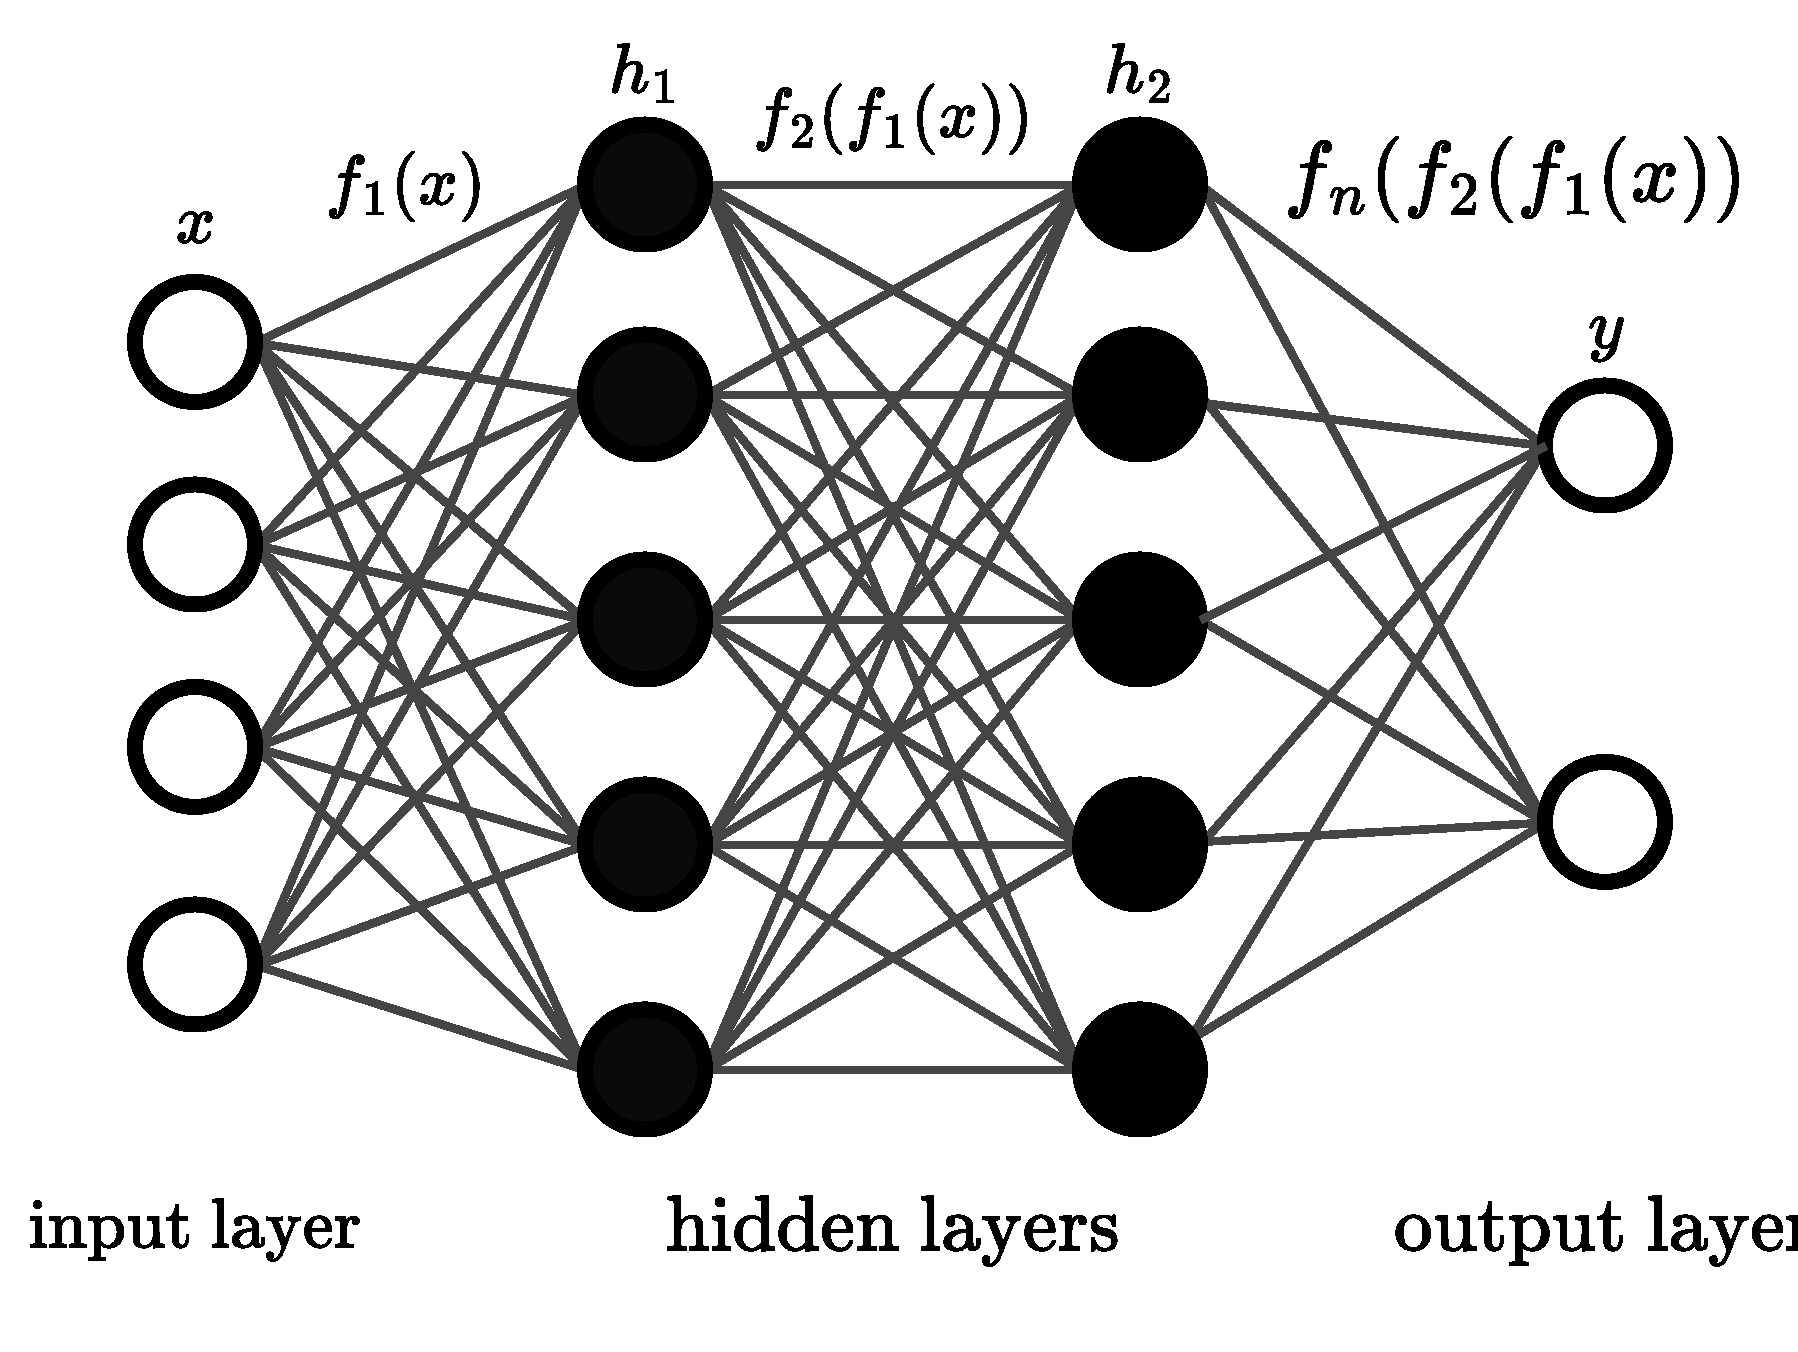
\includegraphics[width=0.65\textwidth]{neural-net.pdf}
  \caption{A 4 layer feedforward network modeling $y = f_{n}(f_{2}(f_{1}(x)))$. The activations of the input layer are set to the value $x$. The values pass from left to right through hidden layers $h_{1}$, $h_{2}$, and finally, the output layer $y$ whose activations represent the model's prediction.}
  \label{fig:ff}
\end{figure}

\medskip
The linear layer is a cornerstone of neural networks. It computes a linear transformation like this:

\begin{equation}
  y = x^{T} \cdot w + b
\end{equation}

where $w$ and $b$ together represent $\theta$. $w$ is commonly referred to as a \emph{weight} and serves to dim or amplify the activation coming from a particular connection, and $b$ \emph{bias} gives the neuron a tendency towards being more or less activated. $x^{T}$ is a transposed vector of activations from neurons of the previous layer, and finally $y$ it the output vector of activations.

Another important layer is the non-linear layer. Which is essentially the same as the linear transformation, except a non-linear function processes its output. Activation of a non-linear neuron can be computed like this:
\begin{equation}
\text{Activation} = \phi\left(\sum_{i=1}^{n} W_{i}x_{i} + b\right)
\label{eq:non-linear}
\end{equation}

$\phi$ is an activation function (such as ReLU), $n$ is the total number of connections from the previous layer to this neuron, $W_{i}$ is the weight of a connection, $x_{i}$ the activation of the connected neuron, and $b$ is the bias value of this neuron. Also see equivalent block diagram \ref{fig:neuron}.

\begin{figure}[ht]
  \centering
  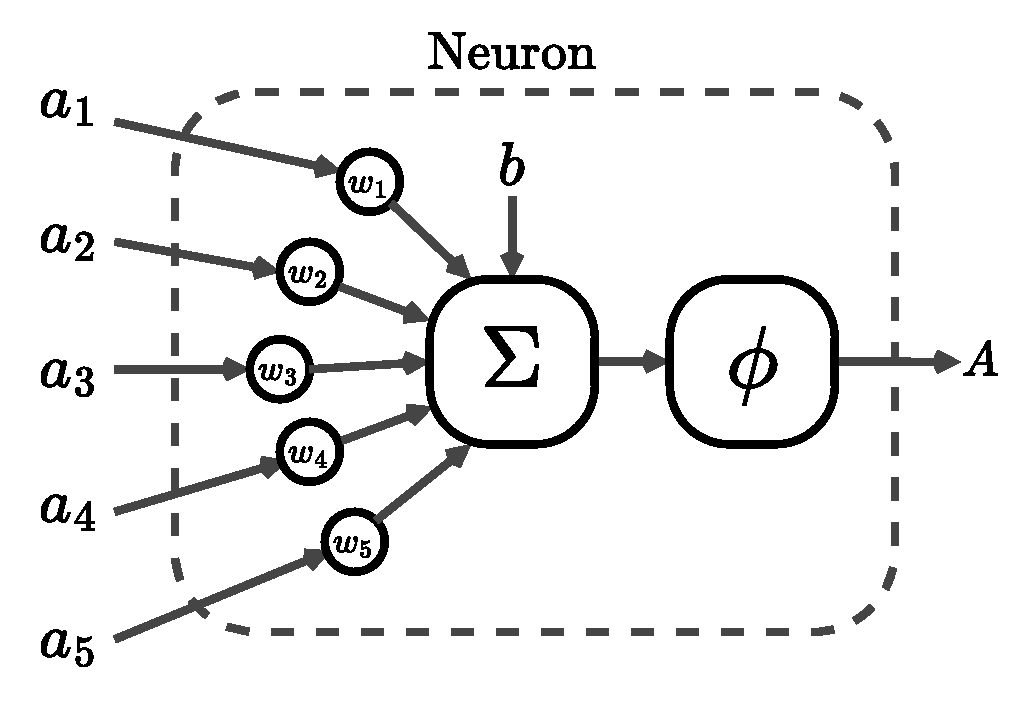
\includegraphics[width=0.6\textwidth]{neuron-connections.pdf}
  \caption{Block diagram of neuron activation calculation, equivalent to equation \ref{eq:non-linear}. $a_{1-5}$ are activations from all neurons in the previous layer. $a_{1-5}$ each get multiplied by their respective weights $w_{1-5}$ and the results are summed together with a bias parameter $b$. This sum is then processed by an activation function $\phi$, whose output is the neuron's activation. }
  \label{fig:neuron}
\end{figure}

\subsection{Training Neural Networks}

An obvious challenge when working with a neural network is obtaining suitable values for $\theta$. One approach used historically is manual tuning with the help of field experts. This approach is problematic as it requires extensive amounts of time and effort. And once training is done, very little progress can be shared with projects from different domains.

The model is trained by first running an inference. This is called the \emph{forward pass}. During the forward pass, the state of every layer is saved in a \emph{computational graph}. A \emph{cost function} is then used to calculate an error score between the model's output and the labels. This value is called a \emph{loss}. An \emph{optimization algorithm} such as \emph{back-propagation}\,\cite{BackProp1986} takes the computational graph obtained during the forward pass and, with the help of the \emph{chain rule}, computes gradients for each function, starting from the loss calculation, and going all the way to the input layer as shown in \ref{fig:back-prop}; this is called a \emph{backward pass}.

Naturally, the gradient represents the direction in which the parameter $\theta$ needs to be adjusted to increase the loss value, so by subtracting a fraction of the gradient from parameters $\theta$, the model's performance on the current sample improves. This is called \emph{gradient descend}. This process repeats until the model stops improving. Before the training starts, the parameters $\theta$ are typically initialized with random noise of low yet non-zero values.

\begin{figure}[H]
  \centering
  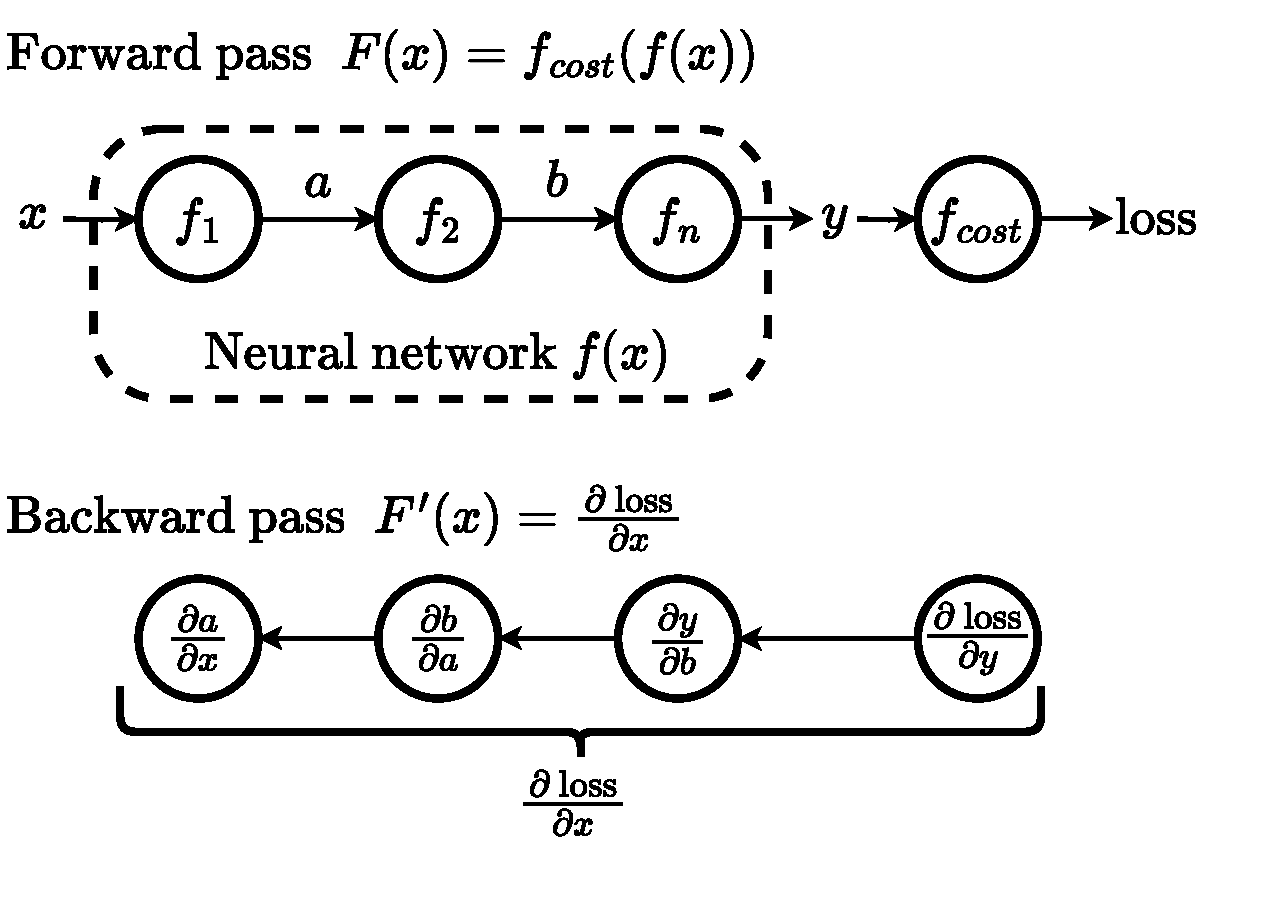
\includegraphics[width=0.75\textwidth]{neural-net-backprop.pdf}
  \caption{Forward pass and backward pass are shown side by side. During the forward pass $F(x)$, the function of the neural network $f(x)$ is computed along with its loss using $f_{cost}(f(x))$. Gradients can be obtained by deriving the forward pass $F'(x)$. By repeatedly applying the chain rule, the gradient for each function is calculated from the last to the first layer.}
  \label{fig:back-prop}
\end{figure}

The most popular cost function is cross-entropy between the model's outputs and labels. A form of cross-entropy that is widely used in multi-class classification tasks is the \emph{negative log likelihood} of an output layer with softmax\footnote{Softmax normalizes neuron activation in a layer so that their sum is $1$.} applied against the labels.

The negative log-likelihood is calculated as follows:

\begin{equation}
  \text{loss} = -\sum_{i=1}^{N} \log(p(y_i))
\end{equation}

$N$ is the number of processed samples, $y_{i}$ is the label value for $i^{th}$ sample, $p(y_i)$ is the predicted value for $i^{th}$ sample.

The network's architecture is integral to its performance. The ideal configuration will differ between applications. Configuration options include the number and types of layers, as well as the number of neurons inside them, the learning rate (gradient multiplier), and various regularization techniques.

\medskip
To make the neural network useful outside of the training examples, it is necessary to ensure that the model is only learning general patterns in the data and not memorizing the individual samples. Performance on unseen data can be tracked with an \emph{evaluation dataset} that contains unique samples and periodically runs inference on it without optimizing. A situation where the performance on the training dataset continues to improve, but the performance on the evaluation dataset remains stagnant or worsens is called \emph{overfitting}.

The opposite would be \emph{underfitting}, where the model stops improving before outputting satisfactory results.

%% ===========================
%%  ____        _
%% |  _ \  __ _| |_ __ _
%% | | | |/ _` | __/ _` |
%% | |_| | (_| | || (_| |
%% |____/ \__,_|\__\__,_|
%%  ____                                     _        _   _
%% |  _ \ ___ _ __  _ __ ___  ___  ___ _ __ | |_ __ _| |_(_) ___  _ __
%% | |_) / _ \ '_ \I '__/ _ \/ __|/ _ \ '_ \I __/ _` | __| |/ _ \I '_ \
%% |  _ <  __/ |_) | | |  __/\__ \  __/ | | | || (_| | |_| | (_) | | | |
%% |_| \_\___| .__/|_|  \___||___/\___|_| |_|\__\__,_|\__|_|\___/|_| |_|
%% ===========================
\chapter{Natural Language Processing}
\label{sec:data_representation}
After learning about the intricacies of neural networks, it is important to show how written text can be passed in and out. This chapter will shed light on tokenization and embedding, which divide the text into smaller segments and encode it into a numerical representation that captures its original meaning. This allows computers to gain an understanding of language. Word embedding essentially bridges the intuition of a neural network and the nuances of words.

As stated in the previous chapter, a neural network has a limited number of input and output neurons, while textual data, such as code snippets, generally vary in length. Therefore, Mapping text to a neural network is not a trivial problem. This chapter will explain how the process of tokenization can be used to encode data for use with neural networks. Unless stated otherwise, information in this chapter is based on the book\,\cite{SpeechLanguageFeb2024}.

\medskip

Tokenization is the most common method for encoding text for neural networks. This approach splits the source text into chunks, called tokens, according to a token vocabulary. Text processing models typically have an \emph{embedding layer} which maps each token in a sequence to a vector, see \ref{fig:embed}.

\begin{figure}[ht]
  \centering
  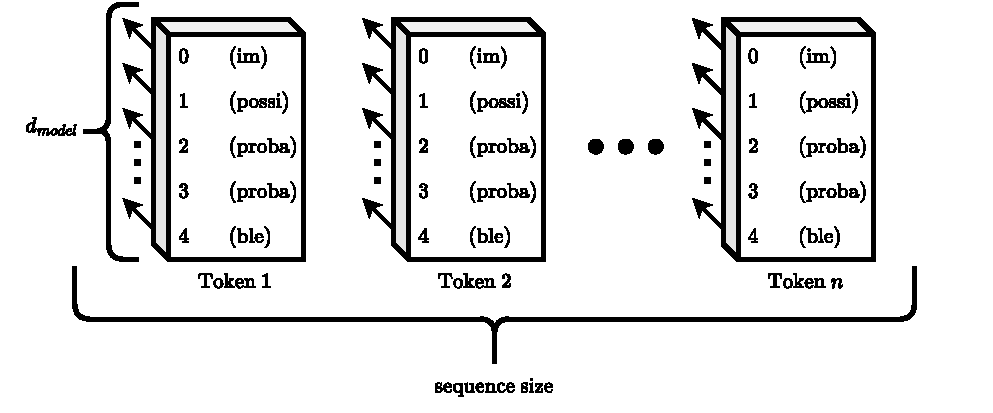
\includegraphics[width=0.85\textwidth]{embedding_layer.pdf}
  \caption{The embedding layer. Each rectangle represents one token slot of the embedding layer. Each slot outputs a feature vector of length $d_{model}$ that is fed into the following layer. The total amount of token slots is called sequence size. }
\label{fig:embed}
\end{figure}

%%% Word2Vec time
\section{Word Embedding}
Creating efficient word vector mappings was a challenge in the field of NLP for a long time until the invention of the Word2Vec model, which, for the first time, properly captured the semantic features of a word, which together represent the overall meaning of the word\,\cite{mikolov2013efficient}. For example, there might be a unit that is correlated with whether the token pertains to a living or unliving object or a value indicating its sex \ref{fig:clustering}.

Word2Vec uses two algorithms to train a shallow neural network for word-to-vector mapping\,\cite{mikolov2013efficient}:
\begin{itemize}
        \item \emph{Continuous Bag Of Words (CBOW)}: This algorithm predicts a hidden word based on the surrounding context without the knowledge of the word order.
        \item \emph{Skip-Gram}: This algorithm is exposed to one word and tries to predict its surrounding words.
\end{itemize}

%%% DIAGRAM clustering
\begin{figure}[]
  \centering
  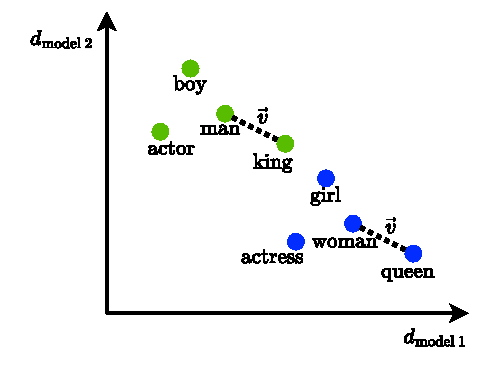
\includegraphics[width=0.6\textwidth]{clustering.pdf}
  \caption{Visualization of some well-trained token-to-feature mapping in two dimensions. Words related to men and women are clustered, respectively. Note that equivalent words in each cluster are spaced similarly. Such as the distance between man and king and woman and queen, which are both $\vec{v}$.}
  \label{fig:clustering}
\end{figure}

Interestingly, with a well-trained embedding mapping, it becomes possible to do arithmetic operations with the semantics of the tokens\,\cite{mikolov2013efficient}:

\begin{equation}
  \text{Embed}(\text{king}) - \text{Embed}(\text{man}) + \text{Embed}(\text{woman}) \approx \text{Embed}(\text{Queen})
\end{equation}

$\text{Embed}$ is a function of the embedding layer, transforming a word into a vector of features. In this example, the symbol ``$\approx$'' denotes a high degree of cosine similarity. Ideally, the difference between the left and right sides of the equation should be smaller than the difference between the right side and the embedding of any other token in the vocabulary\,\cite{mikolov2013efficient}.

By assigning an identification number to each token, the original text can be represented as a sequence of integers. Therefore, The input to the embedding layer can be a simple list of integers. The dimensionality of the embedding layer's output is called $d_{model}$ or sometimes \emph{feature size}.

The length of the sequence that the model can process at once is called the \emph{sequence size}. The number of available tokens is called \emph{vocabulary size}.

\section{Tokenization}
As was shown, tokenization is a powerful approach that enables us to feed textual data in and out of neural networks. However, in order to use tokenization, the vocabulary must be built first. It can have a significant impact on the performance of our model, so it is important to choose the right approach to generating it.

The most obvious solution might be to take the entire dictionary and make it our vocabulary. This approach is not ideal because the number of dictionary words is too large. During the training, less common words might not receive enough attention to develop their embedding mappings properly. This can be solved by removing less common words and representing their occurrences in the data with a generic \texttt{unknown} token, though this is obviously not a great solution either, as this results in the complete loss of meaning of those rare words.

Another obvious strategy would be to go for as minimal vocabulary as possible. Instead of including all possible words, all possible characters may be included. This approach even allows us to encode words from multiple languages and made-up words. However, with this approach, the advantages of vectorized representation are essentially forfeited because the neural network will have to learn to spell; this ultimately reduces learning potential.

In practice, vocabularies are usually created from the same datasets that will be used to train the neural network. There are two main approaches to generating vocabularies: \emph{top-down} and \emph{bottom-up}.

\subsection{Top-down}
With a top-down approach, a set of rules is defined and applied to the dataset, dissecting it into smaller and smaller pieces. Besides a simple conversion to token equivalents, the top-down approach often contains rules that change the text in some way, for example, expanding clitics\footnote{An example of expanding a clitic could be: $\text{don't} \rightarrow \text{do not}$}, removing certain punctuation, and so on. Top-down methods can often map multi-word entities to a single token, like \emph{New York}. One popular top-down approach is the Penn Treebank tokenization standard\,\cite{marcus-etal-1993-building}. In practice, regular expressions are often utilized to implement the rules, as they are deterministic and can be quite fast.

Some issues with the top-down approach arise when trying to parse languages that do not make use of spaces, such as Japanese and Chinese. For the Chinese, a character-based tokenization approach often yields superior results than other methods. In the case of Japanese, specialized word segmentation algorithms are needed.

\subsection{Bottom-up}
The bottom-up algorithm starts by examining the individual characters and applying rules to join multiple tokens to create one that covers more characters. Bottom-up tokenizers include tokens smaller than words, called sub-words. Among popular tokenization algorithms used today are unigram language modeling\,\cite{kudo-2018-subword} and byte-pair encoding\,\cite{sennrich-etal-2016-neural}.

\medskip

Byte-pair encoding was originally introduced as a compression algorithm\,\cite{bytePair1994}, but it was found to have great results as a tokenization algorithm.

The algorithm first adds all unique characters into the token vocabulary. Iteratively, it finds the most commonly occurring sequence of two tokens. It then adds a new token to the vocabulary representing the two tokens together and replaces all occurrences of these two tokens with the newly created one. This repeats until the quota on the total number of tokens is met. The algorithm doesn't cross spaces and, therefore, doesn't include any multi-word entities. Space itself is treated as a character that neighbors only the character to its left\,\cite{sennrich-etal-2016-neural}.

Provided that all possible tokens for a given task are included in the training set, the model avoids the use of the \texttt{unknown} token since, in the worst-case scenario of encountering a new word made up of unique parts, it can always be spelled using characters and sub-word tokens, but more common words and sub-words are still able to enjoy the benefits of semantic feature representation.

\medskip

During regular encoding, the tokenizer uses a greedy version of this algorithm, aiming for the longest token found in the vocabulary. Decoding is trivial, each token is mapped to its equivalent characters.

The idea behind bottom-up algorithms such as this one is that individual sub-word units ``morphemes'' will end up as tokens. For example, improbable consists of ``im'', which serves as a negation; ``prob'', the root which relates to the concept of probability; and ``able'', which is used to turn verbs into adjectives as shown in \ref{fig:embed}.

%% =============================================================
%%  _____                 __
%% |_   _| ___ _ _ _ __  / _| ___  _ __ _ __ ___   ___ _ __ ___
%%   | || '__/ _` | '_ \I |_ / _ \I '__| '_ ` _ \ / _ \ '__/ __|
%%   | || | | (_| | | | |  _| (_) | |  | | | | | |  __/ |  \__ \
%%   |_||_|  \__,_|_| |_|_|  \___/|_|  |_| |_| |_|\___|_|  |___/
%% =============================================================
\chapter{State of the Art}
\label{sec:llm}
This will go over \emph{Large Language Models (LLM)}, a technology utilizing neural networks with many layers to perform intelligent language processing. Starting with a short summary of the RNN-based models, followed by the introduction of attention, which is a core mechanism in Transformer-based models that recently revolutionized this field. 

Transformers are a family of Large Language Models based on the architecture of the original Transformer model created by Google in 2017. When first introduced, it outperformed all other contemporary machine-translation technologies by a significant margin. 

\medskip
% - attention
The invention of the transformer was preceded by the discovery of the attention mechanism described in\,\cite{bahdanau2016neural}. This paper introduced a novel technique for then-popular RNN-based architecture called \emph{Long Short-Term Memory LSTM}\,\cite{lstm1997} and its improved variant, the \emph{Gated recurrent unit GRU}\cite{gru2014} architecture. 

\medskip

Information in this chapter is primarily based on the book\,\cite{SpeechLanguageFeb2024} while information pertaining directly to the Transformer model is based on its foundational paper\,\cite{Transformer2023}.

\section{Recurrent Neural Networks}

Language processing with RNN-based neural networks suffers from poor context memory. Information stated earlier in the text is often forgotten, and too much weight is placed on recent parts of the sequence. In practice, this manifests as a drop-off in accuracy as the sequence size grows. This problem stems from the structure of the network itself; see \ref{fig:rnn}.

\begin{figure}[ht]
  \centering
  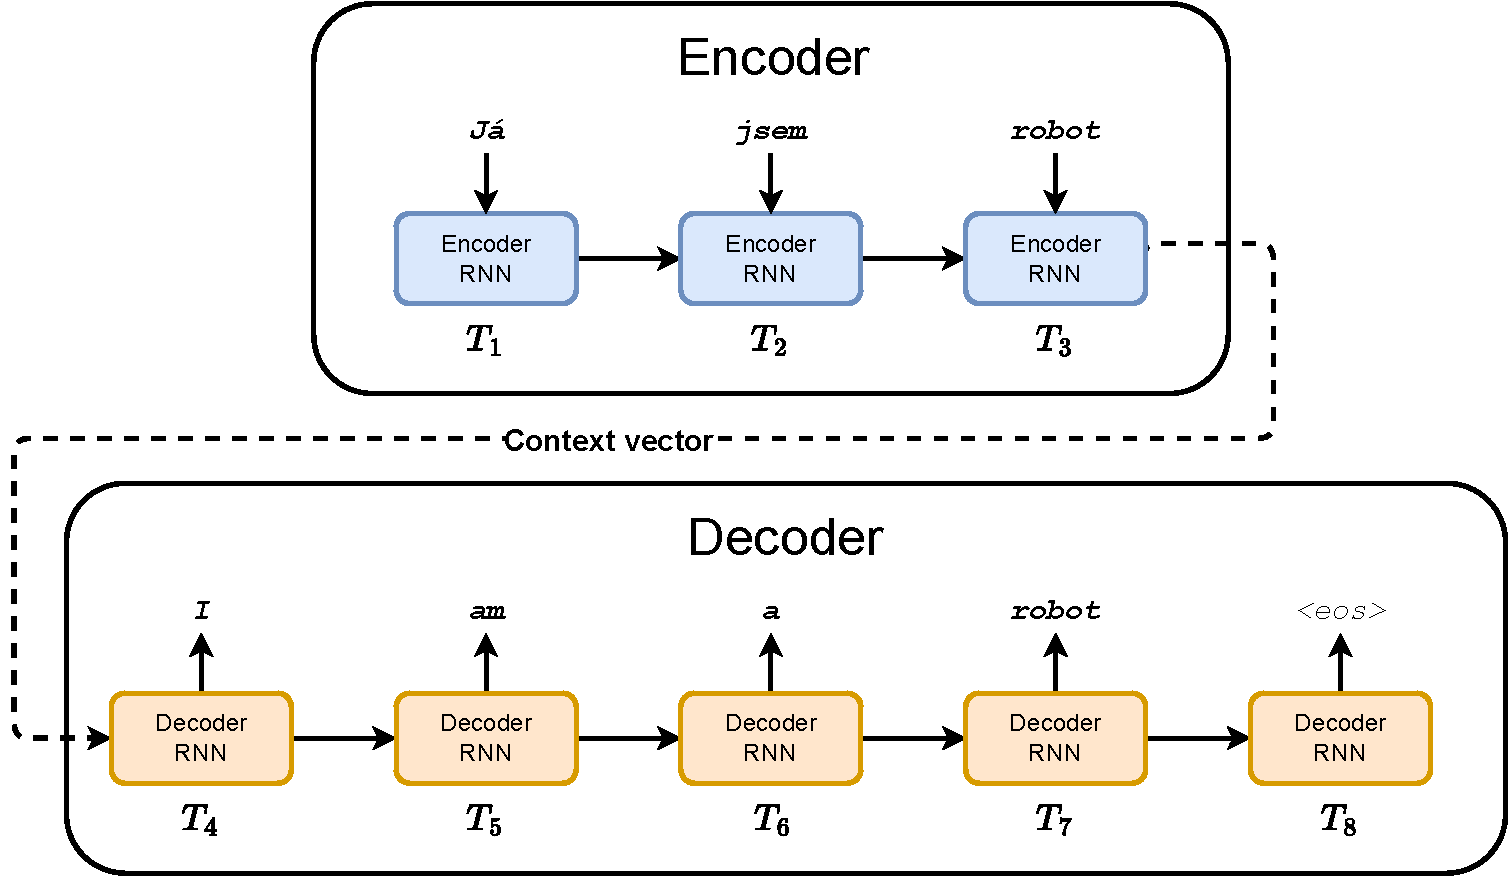
\includegraphics[width=0.66\textwidth]{encoder-decoder.pdf}
  \caption{
    Diagram of an RNN-based model performing a sequence-to-sequence translation. The model consists of two parts: an encoder and a decoder. Time steps are denoted as \(T_{n}\). Each input token is processed sequentially by the encoder RNN. The encoder receives the state from the previous time step and the current token as inputs.
    After all input tokens are processed, the encoder's final state is given to the decoder as an initial state.
  The decoder is an RNN for output generation; it repeatedly processes its previous state and outputs a token. The decoder iterates until the model generates an \texttt{end of sequence} (\texttt{<eos>}) token or some other condition is fulfilled.
  }
  \label{fig:rnn}
\end{figure}

Since the state is continually updated by newer inputs, information about older tokens gets overshadowed by information from later networks. LSTM has improved with this issue by introducing a gating mechanism\,\cite{lstm1997}, enabling the model to selectively retrain or forget information. Despite this advancement, this challenge was not fully overcome. The following paragraphs will describe the attention mechanism, which allows further improvements in context memorization.

\section{Attention}

Attention helps determine which parts of the input are relevant to the current state. Attention can be implemented in LSTM models by adding a third input to the decoder. First, all encoder states need to be saved. While decoding is underway, each of those states is concatenated with the decoder state and passed through a non-linear, fully connected layer. The results are scalar values representing the relevance scores of each input token in relation to the decoder state. The final context vector, which is the attention's output, is calculated as a sum of all encoder hidden layers scaled by their normalized attention scores. This kind of attention is called additive decoder attention\,\cite{sennrich-etal-2016-neural}.

\medskip

\section{The Transformer Model}
% - self-attention
The discovery of attention then led to an even larger breakthrough in the field of LLM when it was discovered that the properties of RNNs that made pre-attention language models so performant were now holding it back. Researchers at Google found that by complementing the attention mechanism with only a single-layered feed-forward network, the model was able to outperform competition in translation tasks without needing more complex components. The transformer was also computationally faster since it could be easily parallelized, thanks to the absence of feedback connections.

\begin{figure}[ht]
  \centering
  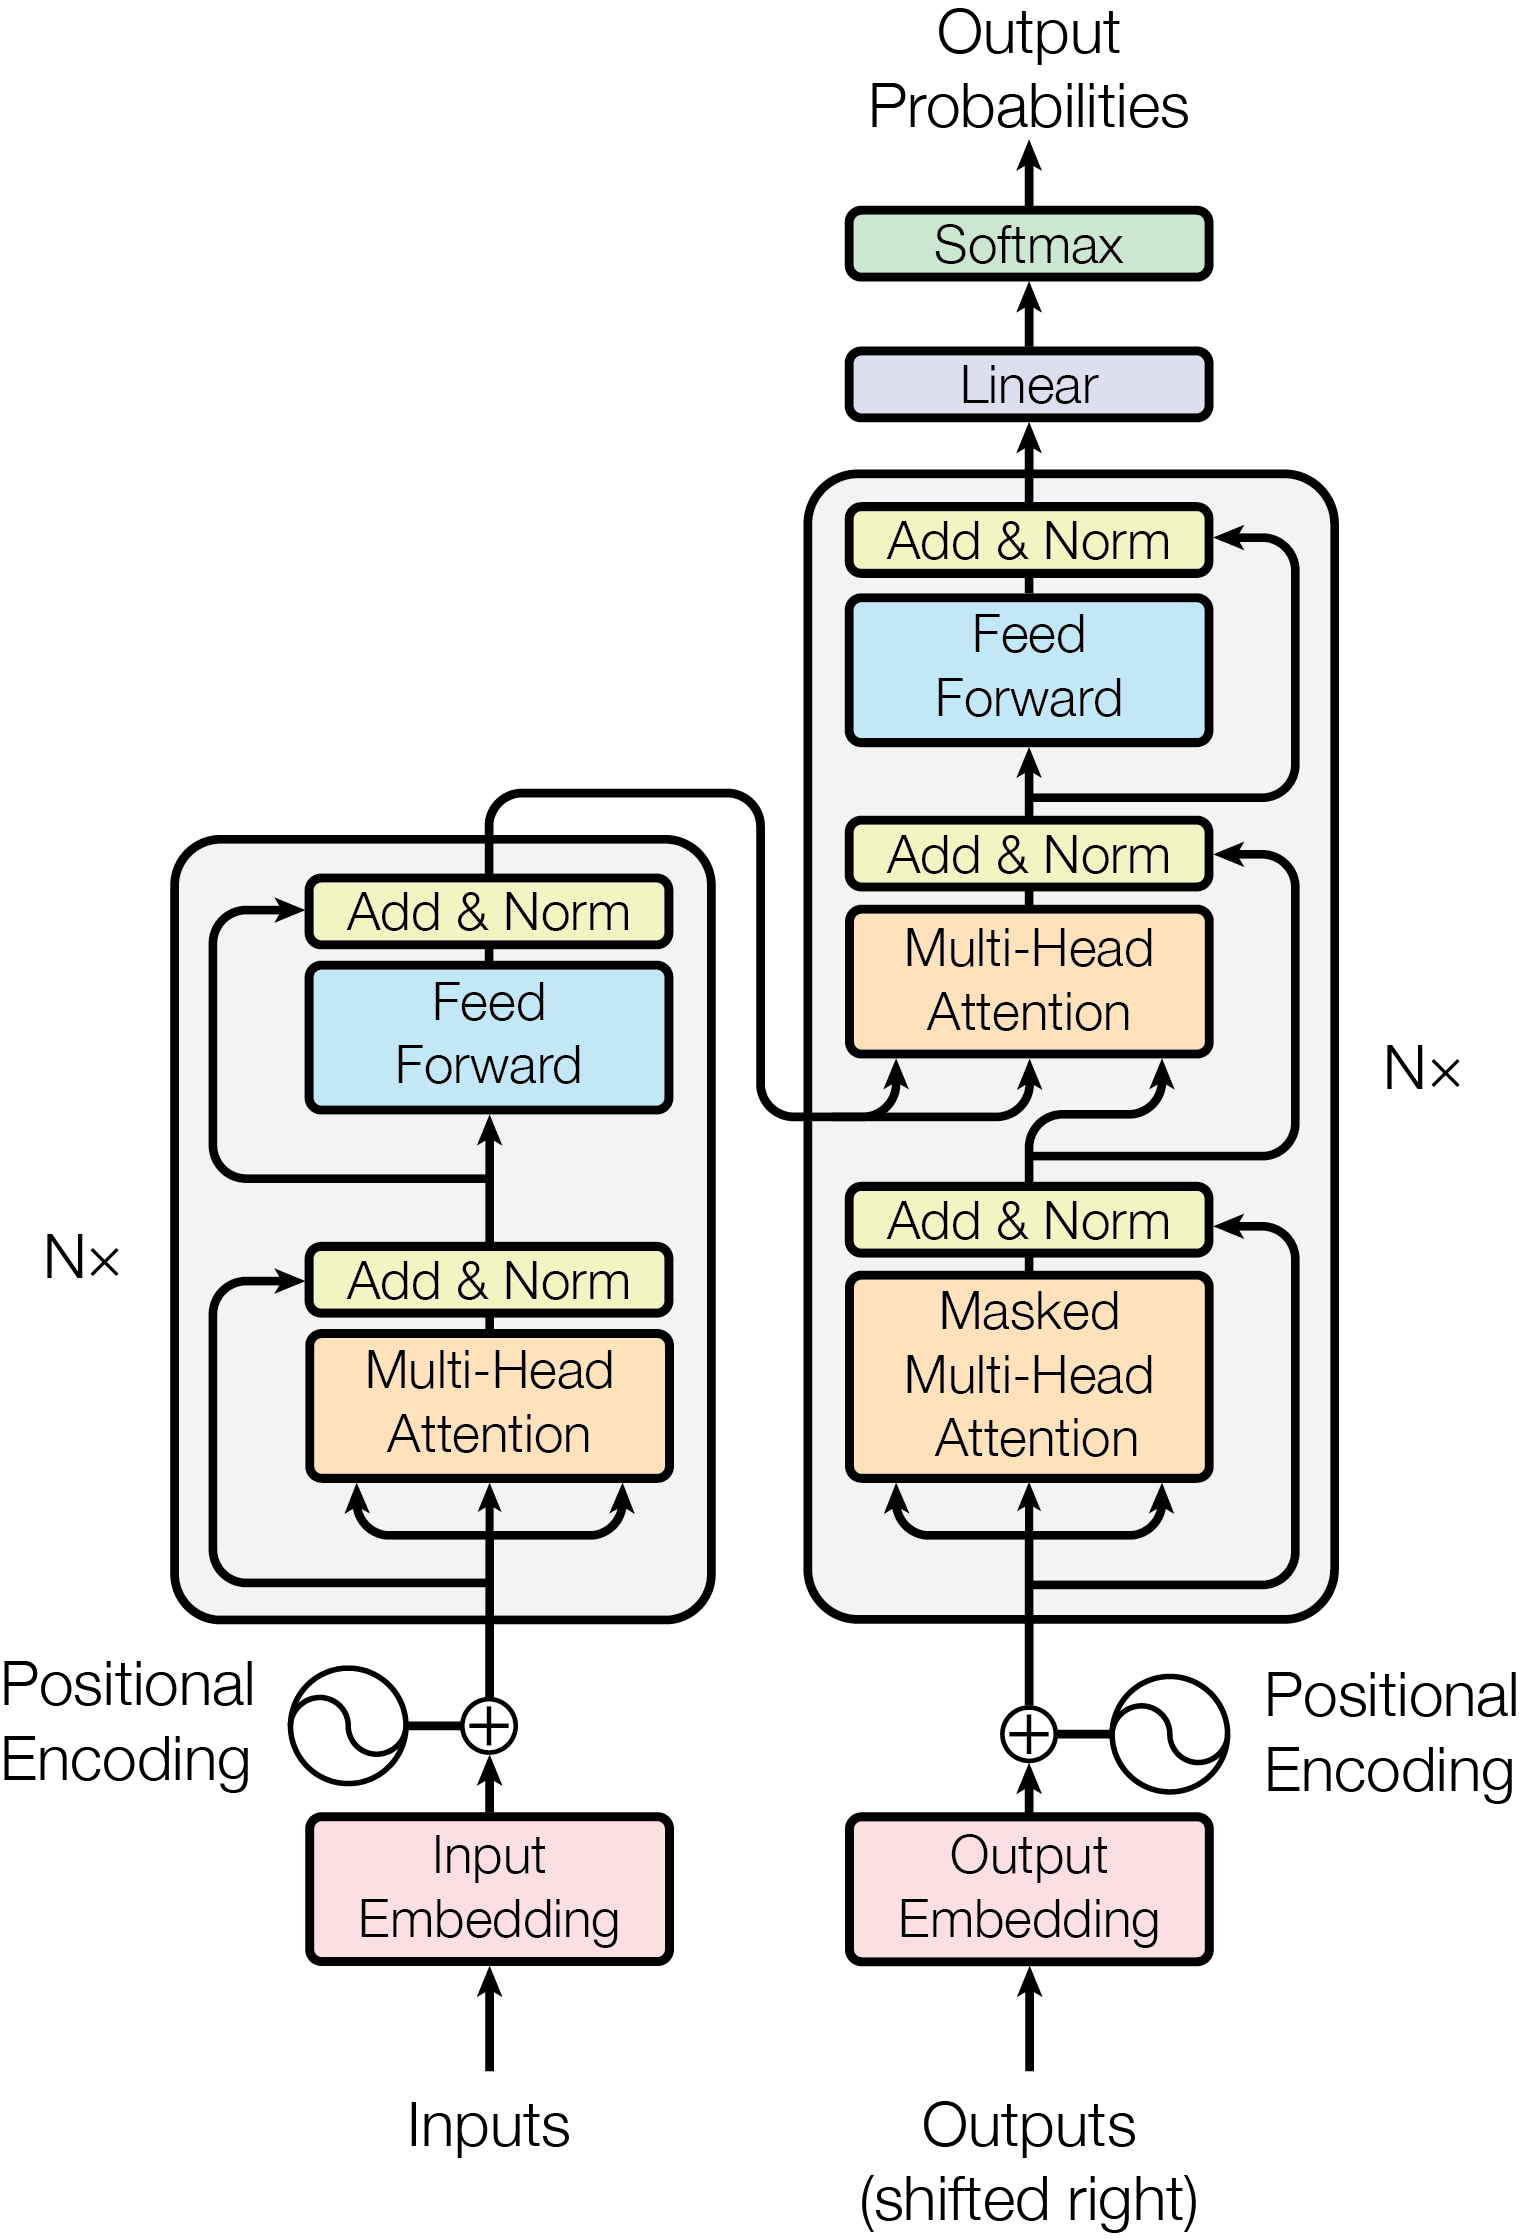
\includegraphics[width=0.53\textwidth]{ModalNet-21.png}
  \caption{The original transformer model. The encoder is depicted as the large block on the left and the decoder as the large block on the right. The encoder receives embedded input tokens with positional encodings, processes them, and gives its output to the decoder, which receives previously outputted tokens as input. The decoder's final hidden layer is used to determine the output token using the linear and softmax layers. This diagram was taken from Transformer's foundational paper\,\cite{Transformer2023}.}
  \label{fig:transformer}
\end{figure}

The transformer model uses its own variant of the attention mechanism, called \emph{multi-head self-attention} (figure \ref{fig:attention}). The attention formula itself is called \emph{scaled dot-product attention}. This method is called self-attention because it compares the input tokens with one another. The attention is calculated with the help of three intermediate matrices: \emph{Query $Q$, Key $K$ \emph{and} Value $V$}. Each is obtained by running the feature vector through a linear layer. The attention is calculated as follows:

\begin{equation}
  \text{Attention}(Q, K, V) = \text{softmax}(\frac{Q \cdot K^{T}}{\sqrt{d_{k}}})\cdot V
\end{equation}


$d_{k}$ is the dimensionality of $K$ and $Q$. In this case, the resulting attention is not a scalar but a vector of the same dimensions as the initial feature vector. This constitutes self-attention with a single head. When using multiple heads, the feature vectors are split so that every head processes an equal portion of the input. The output from the heads gets concatenated to restore its original dimensions.

\begin{figure}[ht]
  \centering
  \begin{subfigure}[t]{0.3\textwidth}
    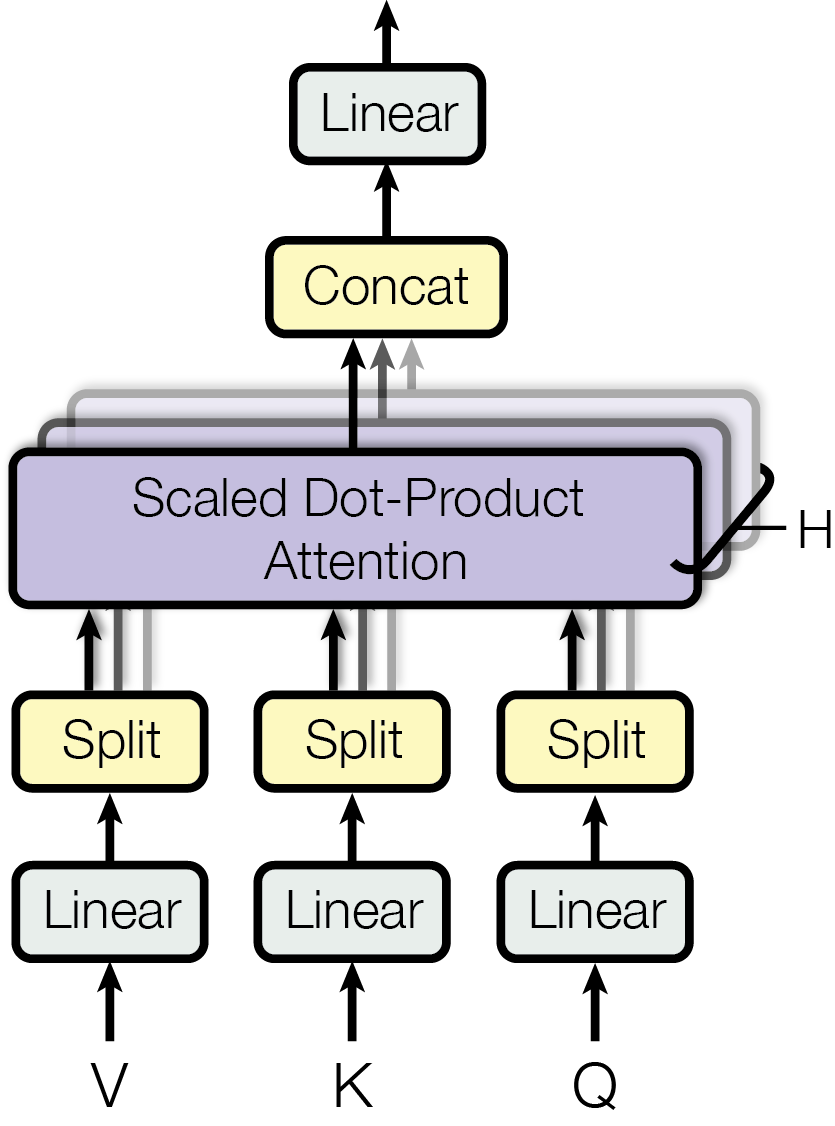
\includegraphics[width=\textwidth]{ModalNet-32.png}
    \label{fig:attention_a}
    \caption{}
  \end{subfigure}
  \hspace{3cm}
  \begin{subfigure}[t]{0.2\textwidth}
    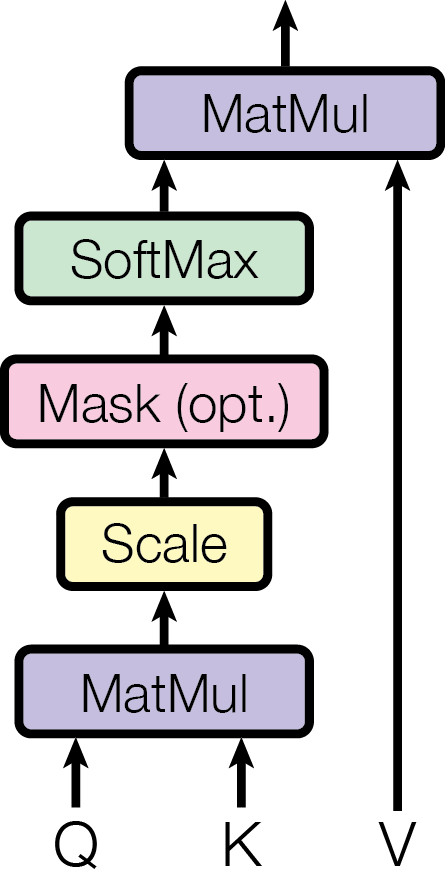
\includegraphics[width=\textwidth]{ModalNet-19.png}
    \label{fig:attention_b}
    \caption{}
  \end{subfigure}
  \caption{Attention block diagram. Image (a) is a diagram of multi-head self-attention, and image (b) is a diagram of \emph{scaled dot-product attention} calculation.}
  \label{fig:attention}
\end{figure}

\begin{figure}[ht]
  \centering
  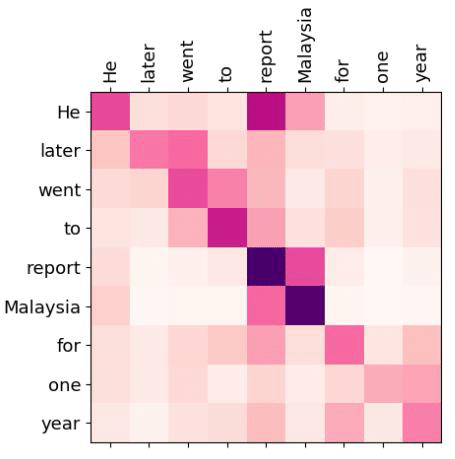
\includegraphics[width=0.40\textwidth]{attention-matrix.png}
  \caption{Example of a visualization of a self-attention matrix. Darker colors represent high activations. Note strong activation between semantically related tokens such as \emph{He} and \emph{report}. This figure was taken from\,\cite{attention-matrix}.}
  \label{fig:attention-matrix}
\end{figure}

One factor in which Transformers differ from earlier architectures is that the sequence size stays fixed after training. This is due to positional encoding, which is a mechanism that gives the transformer a sense of the order of the tokens. The position is encoded by adding a sine wave to even units of the vector and a cosine wave to the odd ones, with the frequency of the wave communicating the position. Like so:

\begin{equation}
PE(p,i) = g(p/10000^{{2i/d_{model}}})
\end{equation}

where $p$ is the token position, $i$ is the dimension in the vector and $g$ can be sine or cosine.

\medskip

% - encoder-decoder
The transformer uses an \emph{encoder-decoder} framework (figure \ref{fig:transformer}), also known as \emph{sequence-to-sequence (seq2seq)}, which was originally developed for the earlier RNN-based models. It splits the model into two parts: the first is called the \emph{encoder}, and the other is the \emph{decoder}. As the name suggests, the goal of this model is to transform one sequence of text into another. This architecture is useful for translations, where a sentence in one language is supplied as the input, and the sample sentence is translated into a different language as the label.

\subsection{Encoder}
% - encoder
The encoder receives the token embeddings with the positional encoding of the input sequence from the embedding layer. The encoder block typically repeats several times, six times in the original paper, but each time it uses different parameters.
\medskip
The encoder is centered around a residual pathway leading from the input to the output, providing a relatively unobfuscated path from the cost function to every trainable parameter to ensure strong gradients for all weights and biases. The residual pathway is first sampled by the \emph{Multi-head Attention}, which processes the feature vectors and then returns its output to the residual pathway. The addition is used to join processed outputs to the residual path and to prevent values from becoming too large; the residual pathway is then normalized.

The next in line to sample the pathway is a feed-forward network with one hidden layer. This layer typically has more neurons than input dimensions to capture more complex relationships. The output from the feed-forward then joins back with the residual pathway with addition and normalization, just like before.

The encoder's output captures the overall meaning of the input, often called the \emph{context}. It can either be paired with a decoder to perform sequence-to-sequence transformations, or it can be used for tasks such as sentiment analysis, classification, or searching.

\medskip

\subsection{Decoder}
% - decoder
The decoder runs interactively, each time generating a single token based on the context provided by an encoder.
A decoder block is not too different from an encoder; it is also built around a residual pathway that begins at an embedding layer, where, just like before, tokens are converted to their vector representation and enriched with positional encodings. However, this time, the network is fed a sequence of its own outputs from previous time steps. This provides the decoder with information about previous time steps. Before the first token is generated, the decoder is initialized with a special \texttt{beginning of sentence} token as input.
The output token of the decoder is obtained by passing the last activations from the decoder to a classification head, which is comprised of a linear layer and a softmax layer, where activation of each neuron represents a probability of a token.

The first on the residual pathway is multi-head attention. In this layer, it is crucial to mask out the token that is currently being predicted and all the ones that follow it to ensure that during training, the decoder learns to work only with tokens from the past. Then, the attention is calculated, and the result is merged back to the residual pathway like before.

% - cross-attention
Another operation on the residual pathway is a multi-head cross-attention. This is similar to self-attention, but instead of attending to itself, the decoder state attends to the encoder's output. Lastly, a decoder block ends with a feed-forward with one hidden layer.

Just like encoders, decoders can be used without an accompanying encoder. In this configuration, the cross-attention layer is omitted. Instead, the information about the input is supplied as initial tokens to the input; the decoder then generates new tokens to extend this sequence. This approach is quite popular. Among successful decoder-only models is OpenAI's GPT series.

% - Trénování transformerů
\subsection{Training Transformers}
Training transformers is the same as training any other neural network using gradient descent. The original Transformer uses the Adam (Adaptive moment estimation) optimizer, which is very popular with other Transformer-based model\footnote{Adam is used by BERT\,\cite{devlin2019bert}, GPT\,\cite{gpt32020} and many others.}. The Adam optimizer enhances regular gradient descent by dynamically adjusting the learning rate of each individual weight and bias based on two factors: The momentum of the gradient and the amount of fluctuation of the gradient\,\cite{kingma2017adam}.

A common technique to prevent overfitting is not using a gradient from a single inference but adding gradients from a batch of samples together. The batch gradient is divided by the number of samples in a batch so that the effective learning rate stays the same. Thanks to batching, the gradient is smoother and includes less sample-specific information. It can also be more performance efficient as the calculations of different samples can be done in parallel\,\cite{DeepLearning2016}.

If the input doesn't match the maximum input size exactly, it is necessary to fill the capacity with a special \texttt{padding} token, which is ignored during attention calculations.

% Pretraining
Modern LLMs have anywhere between hundreds of millions\footnote{Bart Base has 140 million parameters\,\cite{bart-2020}.} and billions\footnote{GPT-3 has over 175 billion parameters\,\cite{gpt32020} .} of parameters. Therefore, training them takes a considerable amount of money. Because of this, models are often trained in two phases. First, on general information relevant to a variety of tasks from a given domain, this technique is called \emph{pre-training}, and then they are exposed to a specific task, which is called \emph{finetuning}.

There are various strategies for pre-training an LLM, for example \emph{Denoising Autoencoder DAE} which works by corrupting the input data in some way\footnote{Corruption methods for DAE include: Token Masking, Chaining order of tokens, Removing tokens and others.} and comparing the output to the original text\,\cite{bart-2020}.

% Finetuning
After a model has been pre-trained using general text, it can be trained on a more specialized dataset to perform a specific task. This is called \emph{fine-tuning}. The fine-tuning process takes considerably less time and needs only a fraction of data than training from scratch would require.
A single pre-trained model can be used to fine-tune multiple models.
The inputs and outputs should be formatted the same way they will appear during deployment.

% - Decoding strategies

\subsection{Output decoding}
% sampling
The sampling method determines which token should be chosen as the output of the decoder. Notable ones include:
\begin{itemize}
        \item \emph{Greedy sampling}: The likeliest token is always greedily selected.
        \item \emph{Random sampling}: The output is chosen randomly based on the probability distribution outputted by the model.
        \item \emph{Top-k sampling}: The output is chosen from the $k$ likeliest tokens using random sampling. 
        \item \emph{Top-p sampling}: A pool that is made up of the most likely token up to a cumulative certainty of $p$ is randomly sampled.
\end{itemize}

% searching
Searching is another tactic for choosing the output:

\begin{itemize}
  \item \emph{Greedy search}: This is the simplest approach. At each step, only the likeliest token is chosen every time\,\cite{SpeechLanguageFeb2024}
        \item \emph{Beam search}: The algorithm keeps $n$ most probable sequences that it expands each time step. The output is the sequence with the highest cumulative probability.
\end{itemize}

\chapter{Tools and Technologies}
    
    The models have been trained using \emph{Torch}, a Free machine-learning library for Python that allows efficient tensor computing on the GPU. It also supports dynamic computational graph building, which is crucial for backpropagation. 
    
    Another important library used for the training is the \emph{Huggingface Transformers library}. It provides a unified framework for sharing models of different architectures while retraining a fine grip over the training process. Huggingface offers a library of Models of other architectures. Transformers library significantly streamlines the experimentation process of comparing different models in otherwise identical conditions, which is much more difficult while working with raw Torch models.

    Other Python libraries used in the project: \verb|SentencePiece|, \verb|toml|, \verb|accelerate|, \verb|astor|, \verb|peft|,  \verb|datasets|, \verb|bitsandbytes|, \verb|tqdm|, \verb|json|, \verb|nltk|, \verb|logging|, \verb|sacrebleu|.
    
    In order to train and evaluate the models, The Faculty's compute servers were heavily used, namely: \verb|pkcnot6|, \verb|pkcnot8|, \verb|athena19|, \verb|athena20|.
    
    \section{Sparse Attention Transformers} \label{led}
    % Teorie, důvod použití
    % Longformer, LED
    One of the biggest problems with training large language models is large memory size requirements. This factor often limits the sequence size and the number of parameters.

    The standard Transformer architecture suffers from \emph{quadratic memory complexity} in relation to the increase in sequence size, stemming from the nature of the attention mechanism\,\cite{child2019generating}. This results in very high memory usage, particularly during training where, when using the Adam optimizer, it is required to store one copy of the model, loss averages, loss momentum, and one or more gradients; each has the same memory size as the model. Fortunately, there are some approaches that can help lower memory consumption.

    \medskip
    
    The first one is sparse attention, a concept in which attention is only applied to a subset of the sequence, allowing for a lower memory footprint\,\cite{child2019generating}. Popular architectures include \emph{BigBird}\,\cite{zaheer2021big} and \emph{Longformer}\,\cite{beltagy2020longformer}. This paper makes extensive usage of the ladder. 

        Longformer achieves sparsity of the attention matrix by introducing two separate attention mechanisms, \emph{local attention} and \emph{global attention}.
        
        \begin{itemize}
            \item \emph{Local Attention} computed by a sliding window whose size is a fraction of the maximum sequence length. Local attention ensures that each token is attending to itself and a $w$ amount of tokens before and after. $w$ is the window size. See \ref{fig:sliding-window-attention}.
            
            \begin{figure}[H]
              \centering
              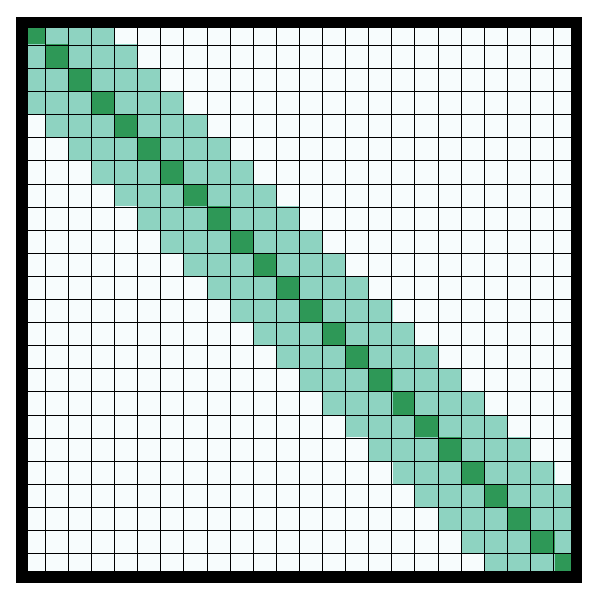
\includegraphics[width=0.4\textwidth]{obrazky-figures/fig-attn-window.pdf}
              \caption{Local attention diagram. The table represents attention between tokens; highlighted squares show that the row and column tokens are attending to each other. With traditional full attention, all squares would have been highlighted. The local attention window effectively reduces the number of attending tokens to a strip around the diagonal. In this particular case, the window size $w$ would be 3. Image taken from the Longformer paper\,\cite{beltagy2020longformer}.}
              \label{fig:sliding-window-attention}
            \end{figure}
            
            \item \emph{Global Attention} compliments local attention by enabling certain hand-picked tokens to attend to the whole input sequence. Allowing the model to better understand long inputs that contain important tokens that affect a larger part of the document. 
            \begin{figure}[H]
              \centering
              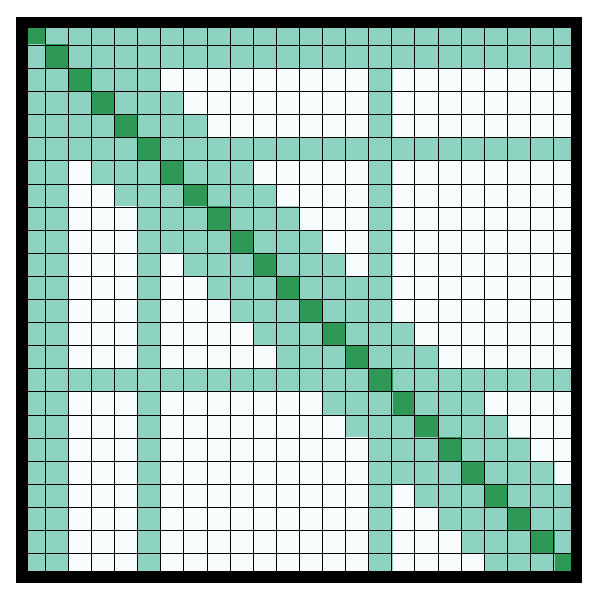
\includegraphics[width=0.4\textwidth]{obrazky-figures/fig-attn-combined.pdf}
              \caption{Local attention and Global attention together. The table represents attention between tokens; highlighted squares show that the row and column tokens are attending to each other. In addition to the diagonal strip, certain tokens are allowed to tend to the whole input like it is in full attention. Taken from the Longformer paper\,\cite{beltagy2020longformer}}
              \label{fig:global-attention}
            \end{figure}
        \end{itemize}

        The Longformer uses separate projection $QKV$ matrices for each Attention mechanism. Longformers architecture is, in a way, an extension of the RoBERTa\,\cite{liu2019roberta} model. In fact, it is possible to use a pre-trained RoBERTa model to \emph{initialize a Longformer}, in which case equivalent parameters are copied, and positional embeddings are extended via tiling. 
        
        The original Longformer model was developed as an encoder-only model, and some have even used it as an autoregressive model\,\cite{guo2023longcoder}. However, the standard version of Longformer \emph{does not support cross-attention}, so a separate model was developed for the purposes of sequence-to-sequence generation.

        \emph{Longformer Encoder-Decoder (LED)} is a sparse attention model that includes both an encoder and a decoder. Similarly to the original Longformer, it is extending a well-known model architecture, in this case, \emph{BART}\,\cite{bart-2020}, and may also be initialized with BART weights.

        \medskip

        This project extensively uses LED models, particularly those initialized with weights and biases of the \emph{PLBART model}\,\cite{ahmad2021unified}, a model trained on natural language and programming language. Thanks to the LED model, CodeImprove uses sequences of up to 2048 tokens despite the fact that PLBART only supports 512. In particular, the model was trained on natural language as well as Python and Java.

    \section{Quantized Low Rank adaptation} \label{qlora}
        Another approach is \emph{QLoRA or Quantized Low-Rank adaptation}\,\cite{dettmers2023qlora}. This technology allows the fine-tuning of very large language models with \emph{billions} of parameters on consumer-grade hardware by dramatically lowering the memory footprint of training.

        \medskip
        
        QLoRA is an improved version of \emph{LoRA (Low-Rank Adaptation)}. 
        
        As described in\,\cite{hu2021lora}, LoRA works by injecting additional parameters known as low-rank adapters into a pre-trained model and solely training those during fine-tuning, see \ref{fig:lora-diagram}. The rationale is that with a pre-trained model, you only need to alter the model a little bit to fine-tune it for a specific task, as most of the core knowledge was already obtained by the base model, and the inserted adapter parameters are simply steering the behavior in a certain direction. Of course, this means that this approach is only viable when fine-tuning.

        LoRA fine-tuning was found to have comparable results to full model fine-tuning and, in some cases, even surpassed it. In certain scenarios, LoRA might be achieving better results because it is not prone to catastrophic forgetting, a phenomenon in which the network quickly loses knowledge that is no longer being reinforced by the training data.

        %% LoRA diagram
        \begin{figure}[ht]
          \centering
          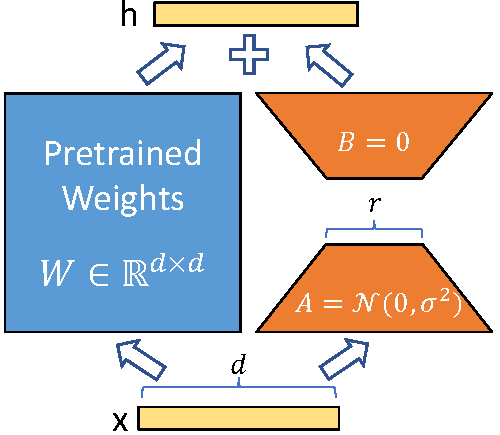
\includegraphics[width=0.5\textwidth]{obrazky-figures/LoRA.pdf}
          \caption{LoRA diagram. $x$ is the output of a previous layer, which is sampled not only by the original layer but also by the Lora adapter shown in orange. Each processes the $x$ in parallel, and the result is summed. $r$ is the size of the LoRA matrix. Figure taken from\,\cite{hu2021lora}.}
          \label{fig:lora-diagram}
        \end{figure}

        However, LoRA becomes even more useful when used alongside quantization. QLoRA is a recently introduced approach to LoRA that reduces parameter sizes to as little as 4 bits per floating-point number. This significantly increases training efficiency compared to the usual 16—or even 32-bit floats.

        To achieve this, QLoRA introduced in\,\cite{June2023qlora} presents a novel data type called \emph{4-bit NormalFloat}. As a 4-bit number, it can hold only 16 distinct states. Each of these states is assigned a value based on the distribution of values in model parameters, as shown in figure \ref{fig:qlora-distribution}. Usually, values of parameters form a normal distribution centered around zero. Parts of the spectrum with values that appear more often have smaller partitions than less populated parts.

        % Quant distribution diagram.
        \begin{figure}[H]
          \centering
          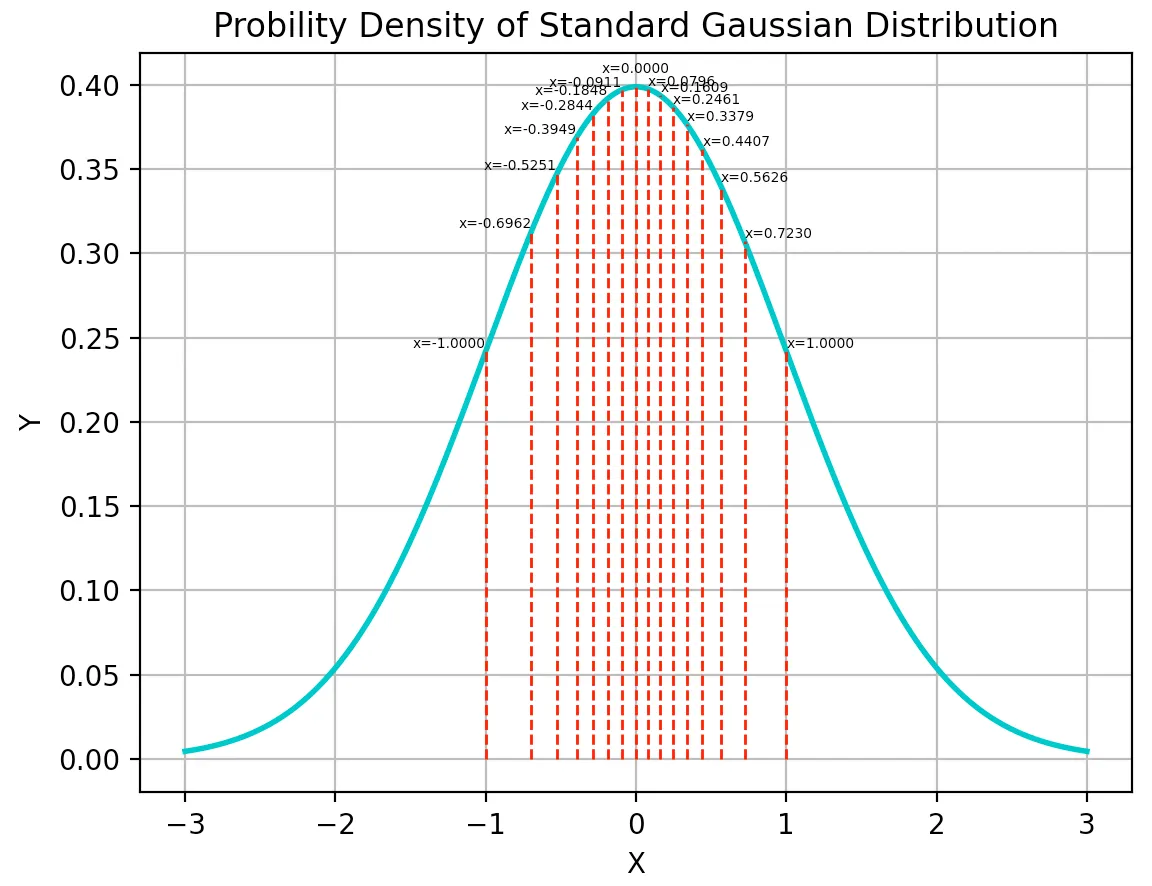
\includegraphics[width=0.8\textwidth]{obrazky-figures/qlora-normal-distribution.png}
          \caption{Example of some distribution of a 4-bit NormalFloat. The distribution of parameter values is in cyan, and the chosen values are in orange. Image taken from\,\cite{June2023qlora}.}
          \label{fig:qlora-distribution}
        \end{figure}
        
        During training, the original weights of the model are kept in their 4-bit form, and adapter weights are used in their 16-bit form, which saves a relatively large amount of memory. During inference, the entire model can be represented with just 4 bits per parameter.

\section{Used Datasets}
    Datasets are an important part of machine learning as their quality can bind the performance of the resulting model. This project makes use of two datasets for training.
    
    \subsection{Error Correction}
        In order to train the error correction module, a custom dataset was assembled from publicly available Freely licensed Python repositories, all of them publicly available on GitHub\footnote{GitHub: \url{https://github.com}}.
        
        Data was extracted from these repositories by first cloning their entire history and then searching commit messages using regular expressions for various iterations of the word \emph{fix}.
        
        A bug fix commit was accepted into the dataset if it contained only one hunk and changed two lines of code or fewer. The changes also had to be contained inside a single function or method body. 
        
        A snippet of the function before the patch, along with the title of the commit message, is used as the input, and the post-patch function is used as the label.
        
        Despite only accepting files ending in \texttt{.py}, it was crucial to conduct additional syntax checks, as many projects have long histories that extend back to Python 2.
        
        \medskip
        
        During this process, it could be observed that large, well-known projects contributed disproportionately more fixes than smaller projects, even if those smaller projects had a long history. This is likely due to the stricter committing etiquette that larger projects enforce, resulting in more concise and atomic commits, which fit the filtering criteria.
        
        Out of the total \emph{1213} repositories, \emph{only 565} contained commits that fulfilled the criteria. The total amount of samples is 16576.
        
        \medskip 
        
        In the pursuit of a larger sample size, the custom dataset is combined with PyTraceBugs\,\cite{pytracebugs}, which focuses on collecting tracebacks and related patches from GitHub issues. The dataset also offers before and after patches of Python functions. As a form of annotation of the samples, the dataset also includes information about the error message the faulty code produced when it crashed.
        
    \subsection{Comments and Rename}

        In order to train the two remaining modules, the \emph{CodeXGLUE code to text dataset}\,\cite{codexglue} was chosen. The main role this dataset fulfills is providing a large base of diverse Python code. The dataset is further reformatted to fit the requirements of both tasks.
    
\chapter{System Design}
    The past few years have seen a sharp influx of machine learning powered tools. Today, there are a plethora of products promising to help programmers with writing code. Among the most popular are GitHub Copilot\footnote{GitHub Copilot: \url{https://github.com/features/copilot}}, Tabnine\footnote{Tabnine: \url{https://www.tabnine.com/}} and Amazon CodeWhisperer\footnote{CodeWhisperer: \url{https://aws.amazon.com/codewhisperer/}}. Many developers also use ChatGPT\footnote{ChatGPT: \url{https://chat.openai.com/}}, which, despite not being marketed specifically towards developers, can handle code-related tasks rather well.
    
    Most of these tools are designed around generative models trained for instruction fulfillment and assistance. They require manual text prompt entry for each task (ChatGPT, GitHub Copilot, Tabnine, CodeWhisperer), where the programmer can specify a question or a task. Often, the AI will have access to the file that is currently open or at least to the highlighted code. Another commonly offered feature is predicting a string of tokens at the current cursor position (GitHub Copilot, Tabnine, CodeWhisperer).
    
    Despite recent technical developments, little has been done in terms of integrating more advanced AI tools into the editor's UI. This would be quite useful, especially for operations that need to be performed frequently and don't need any special details in the prompt. The CodeImprove extension offers such a service, utilizing more economical models for integrated refactoring aid.

    \section{Comment Suggestion Module} \label{comment_suggestion}
        One of the goals of CodeImprove is to enrich the source code with additional documentation in the form of comments. This is a quite complex task, so this work splits it into two parts:
        \begin{itemize}
            \item \emph{Comment detection:} The process of finding what parts of the code need additional documentation.
            \item \emph{Comment generation:} The process of generating the comments themselves.
        \end{itemize}
    
    
    \begin{figure}[H]
      \centering
      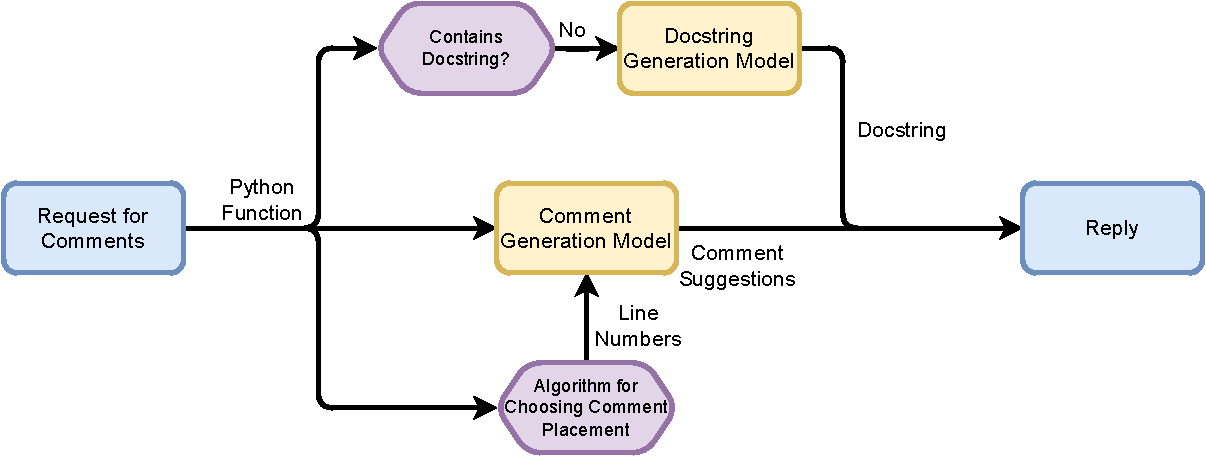
\includegraphics[width=1\textwidth]{obrazky-figures/comment-generation.pdf}
       \caption{Block diagram of the Comment Suggestion module.}
      \label{fig:comment-suggestion-led}
    \end{figure}
    
        \subsection{Comment Detection} \label{comment_detection}
            A docstring is the only kind of comment that has a set placement. The placement of every other comment is completely arbitrary and subject to personal preference.
            
            The initial solution for finding places in need of comments was using an LED model initialized from weights of the PLBart\,\cite{plbart2021} model, trained on the CodeXGLUE code-text dataset\,\cite{codexglue}. Though the dataset is formatted for training models on generating docstrings, it serves as a rich source of Python code that can be further modified to fit other purposes.
            
            In this case, Python's built-in modules \emph{AST} and \emph{tokenize} were leveraged to obtain information about lines that had a comment associated with them, either having a comment at the end of the line or a standalone comment on the line above.
            
            Input is created from the source by removing all of the comments and the docstring and annotating each line with its line number (listing \ref{lst:comment_source}. Global attention is placed on the (\texttt{end of sequence}) token and (\texttt{\_\_python\_\_}) token, and the label is constructed by joining the line numbers of the removed lines (listing \ref{lst:comment_source}).
            
            %% Example of data formatting running dataset_formators.py with global attention.
            \medskip
            \begin{figure}[H]
                \begin{lstlisting}[language=Python, caption={Sample Python code for showcasing dataset formatting. The function calculates $n$ elements of the Fibonacci sequence.}, label={lst:comment}]
    def fibonacci(n):
        """Calculates the Fibonacci sequence of length n."""
        # Initial sequence
        fib_sequence = [0, 1]
        while len(fib_sequence) < n:
            # Add two last numbers from the sequence together
            next_value = fib_sequence[-1] + fib_sequence[-2]
            fib_sequence.append(next_value)
        # Making sure we don't return more than the user has requested
        return fib_sequence[:n]
                \end{lstlisting}
            \end{figure}
            \begin{minipage}{.45\textwidth}
                \begin{lstlisting}[language=Python, caption={Code in listing \ref{lst:comment} formatted as an input for comment detection, italics denote global attention. \\ Note that the code has been ran through the PLBART's preprocessor function, which introduced \texttt{INDENT} and \texttt{DEDENT} tokens, as well as added spacing between tokens.}, label={lst:comment_source}]
    ^\textcolor{teal}{\$ 1 \$}^ def fib onacci ( n ) :
    ^\textcolor{teal}{\$ 2 \$}^ ^\textcolor{gray}{INDENT}^ fib_sequence = [ 0 , 1 ]
    ^\textcolor{teal}{\$ 3 \$}^ while len ( fib_sequence ) < n :
    ^\textcolor{teal}{\$ 4 \$}^ ^\textcolor{gray}{INDENT}^ next_value = fib_sequence [ - 1 ] + fib_sequence [ - 2 ]
    ^\textcolor{teal}{\$ 5 \$}^ fib_sequence . append ( next_value )
    ^\textcolor{teal}{\$ 6 \$}^ ^\textcolor{gray}{DEDENT}^ return fib_sequence [ : n ]
    ^\textcolor{teal}{\$ 7 \$}^
    ^\textcolor{gray}{</s> \textit{\_\_python\_\_}}^
                \end{lstlisting}
            \end{minipage}
            \hfill
            \begin{minipage}{.45\textwidth}
                \begin{lstlisting}[language=Python, caption={Code in listing \ref{lst:comment} formatted as a label.}]
    ^\textcolor{gray}{\_\_en\_XX\_\_}^ 2 4 6
                \end{lstlisting}
            \end{minipage}
            
            After training, the model's results appeared too noisy, primarily generating randomly looking lists of lines. It is possible that instead of learning the intricacies of what makes code require a comment, it was learning average distributions of comments.
            
            \medskip
            
            To get better results, the model was replaced by an algorithm that analyzes the syntax of the code and, through different criteria, chooses places for comment insertion. The heuristic evaluates a line as needing a comment if it contains more than 12 instances of unique identifiers, numbers, or operators in total, if the line was separated by the programmer from the line above by a blank line, or if the line contains one of the following branching control structures: \texttt{for}, \texttt{while}, \texttt{if}, \texttt{try}, \texttt{except}.
            
        \subsection{Comment Generation}
            CodeImprove differentiates between two kinds of comments: a regular hash-symbol (\texttt{\#}) comment, which describes lines that immediately follow it, and docstrings, which are multi-line string literals written at the start of a function or a method block and encapsulate information about the function, docstrings commonly describe what the function does, what each parameter is used for, and what its return value is; docstrings also often include code that showcases how to use the function.
            
            Docstring and comment generation are each handled by a separate model, though they are both trained on the same CodeXGLUE\,\cite{codexglue} code-text dataset as was the abandoned comment detection model; they also fine-tune the LED PLBart model. 
            
            \medskip
            
            When the dataset is loaded, every comment is either removed from the source (80\,\% probability) or kept (20\,\% probability). A sample for training and evaluation is created from each of the deleted comments. Each of these samples shares the same input, that being the source with the comments taken out, with one small change, the location of each comment is marked with \texttt{\$n\$}, where \texttt{\$n\$} is the particular line's number. The label is similarly formatted, starting with this special markup token followed by the content of this comment. The global attention is placed on the function declaration and also on the special markup sequence.

            
            In the case of docstrings, the marking in the input is placed at the very beginning and reads \texttt{\$ DOCSTR type \$}, where \texttt{type} identifies the formatting convention of the docstring and can either be \texttt{GO} for Google's convention\,\cite{GooglePythonStyleGuide}, \texttt{NP} for NumPy's convention\,\cite{NumPyStyleGuide} and \texttt{RE} for the reST convention\,\cite{SphinxPythonDomains}. In the training dataset, these different types of docstrings are classified using regular expressions.
            
            Pylint, TODO, and other kinds of non-descriptive comments are filtered out, along with commented source code, which is filtered by the presence of operators and is normally not included in regular comments.
            
            %% Example of encoded text
            \medskip
            \begin{minipage}{.45\textwidth}
                \begin{lstlisting}[language=Python, caption={Code in listing \ref{lst:comment} formatted as an input for comment generation to predict the docstring. Italics denote global attention. \\ Note that the code has been ran through the PLBART's preprocessor function, which introduced \texttt{INDENT} and \texttt{DEDENT} tokens, as well as added spacing between tokens.}]
    ^\textcolor{teal}{\textit{\$ DOCSTR NA \$}}^ ^\textit{\textcolor{blue}{def} fibonacci ( n ) :}^
    ^\textcolor{gray}{INDENT}^ fib_sequence = [ 0 , 1 ]
    while len ( fib_sequence ) < n :
    ^\textcolor{gray}{INDENT}^ next_value = fib_sequence [ - 1 ] + fib_sequence [ - 2 ]
    fib_sequence . append ( next_value )
    ^\textcolor{gray}{DEDENT}^ return fib_sequence [ : n ]
    ^\textcolor{gray}{</s> \textit{\_\_python\_\_}}
                \end{lstlisting}
            \end{minipage}
            \hfill
            \begin{minipage}{.45\textwidth}
                \begin{lstlisting}[language=Python, caption={Code in listing \ref{lst:comment} formatted as a label.}]
    ^\textcolor{gray}{\_\_en\_XX\_\_}^ ^\textcolor{teal}{\$ DOCSTR NA \$}^ Calculates the fibonacci sequence of length . ^\textcolor{gray}{</s>}^
                \end{lstlisting}
            \end{minipage}
    
            \medskip
    
            \begin{minipage}{.45\textwidth}
                \begin{lstlisting}[language=Python, caption={Another example of code in listing \ref{lst:comment} formatted as an input for comment generation to predict the comment on line 4. Italics denote global attention.}]
    ^\textit{\textcolor{blue}{def} fibonacci ( n ) :}^ 
    ^\textcolor{gray}{INDENT}^ fib_sequence = [ 0 , 1 ]
    while len ( fib_sequence ) < n :
    ^\textcolor{teal}{\textit{\$ 4 \$}}^ ^\textcolor{gray}{INDENT}^ next_value = fib_sequence [ - 1 ] + fib_sequence [ - 2 ]
    fib_sequence . append ( next_value )
    ^\textcolor{gray}{DEDENT}^ return fib_sequence [ : n ]
    ^\textcolor{gray}{</s>}^ ^\textit{\textcolor{gray}{\_\_python\_\_}}^
                \end{lstlisting}
            \end{minipage}
            \hfill
            \begin{minipage}{.45\textwidth}
                \begin{lstlisting}[language=Python, caption={Code in listing \ref{lst:comment} formatted as a label.}]
    ^\textcolor{gray}{\_\_en\_XX\_\_}^ ^\textcolor{teal}{\$ 4 \$}^ Add two last numbers from the sequence together ^\textcolor{gray}{</s>}^
                \end{lstlisting}
            \end{minipage}
    
    \section{Variable Name Suggestion Module}
        Among programmers, one can often hear joking remarks that coming up with names is the most difficult part of the job. CodeImprove aims to help with this issue by suggesting alternative names for variables in case the programmer feels like their creativity did not do a sufficient job.
        
        Because the variable's name is mostly rooted in the code that comes after its declaration, there is little to no point in suggesting code that is still unfinished.
        
        \medskip
        
        The renaming module is powered by a single LED model initialized with PLBART and is also trained on an altered version of the CodeXGLUE\,\cite{codexglue} code-text dataset. 
        
    \begin{figure}[H]
      \centering
      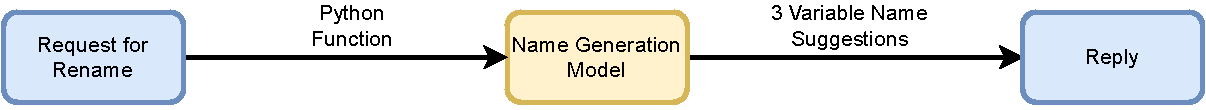
\includegraphics[width=1\textwidth]{obrazky-figures/name generation.pdf}
       \caption{Block diagram of the Variable Name suggestion module.}
      \label{fig:rename-led}
    \end{figure}
    
        Each sample from the dataset is parsed using the \texttt{AST} module. One variable identifier declared within the scope of the function is chosen, and all of its instances are masked out. The original name of the token is used as the label. Global attention is applied to the function definition and to all instances of the \texttt{mask} token.

        \medskip
        \begin{minipage}{.45\textwidth}
            \begin{lstlisting}[language=Python, caption={Example of code in listing \ref{lst:comment} formatted as an input for variable name generation, predicting a new name for \texttt{n}. Italics denote global attention.}]
def fibonacci ( ^\textcolor{teal}{\textit{<mask>}}^ ) :
^\textcolor{gray}{INDENT}^ fib_sequence = [ 0 , 1 ]
while len ( fib_sequence ) < ^\textcolor{teal}{\textit{<mask>}}^ : 
^\textcolor{gray}{INDENT}^ next_value = fib_sequence [ - 1 ] + fib_sequence [ - 2 ]
fib_sequence . append ( next_value )
^\textcolor{gray}{DEDENT}^ return fib_sequence [ : ^\textcolor{teal}{\textit{<mask>}}^ ]
^\textcolor{gray}{</s> \textit{\_\_python\_\_}}^
            \end{lstlisting}

        \end{minipage}
        \hfill
        \begin{minipage}{.45\textwidth}
            \begin{lstlisting}[language=Python, caption={Code in listing \ref{lst:comment} formatted as a label.}]
^\textcolor{gray}{\_\_python\_\_}^ count ^\textcolor{gray}{</s>}^
            \end{lstlisting}
        \end{minipage}
        
    \section{Error Correction Model with LED}
        The error correction feature of CodeImprove is meant to check the programmer's code for small errors and fix them. This module leverages a pair of LED PLBarts to first locate and then fix the errors. This approach is inspired by\,\cite{mashhadi2021applying}.
        
        Fixing errors can be very complex even for experienced programmers; in order to make this task achievable, the models focus on straightforward errors, which can be patched by changing two lines or less.
        
    \begin{figure}[H]
      \centering
      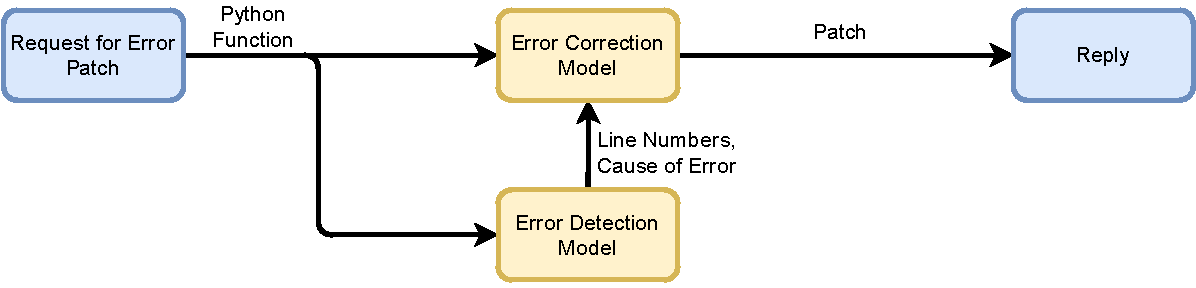
\includegraphics[width=1\textwidth]{obrazky-figures/error correction led.pdf}
       \caption{Block diagram of the Error Correction module using the LED model.}
      \label{fig:error-correction-led}
    \end{figure}
    
    \subsection{Error detection}
        The error detection module judges whether a given snippet contains errors and, if so, locates the lines on which it occurs.
        
        The input is annotated with line numbers enclosed in dollar signs, and the labels are a string of numbers that contain the error separated by spaces.
        
        Of course, not every snippet of code contains errors, and the model should be able to learn that. For this reason, the dataset is supplemented with examples of correct snippets taken from the stable code set of the PyTraceBugs dataset\,\cite{pytracebugs} in the ratio of 1:1.
        
        %%% Example of processed data
            \begin{lstlisting}[language=Python, label={lst:error}, caption={Example of a code snippet with an error. There should be \texttt{append} instead of \texttt{add} as highlighted in red.}]
def fibonacci(n):
    fib_sequence = [0, 1]
    while len(fib_sequence) < n:
        next_value = fib_sequence[-1] + fib_sequence[-2]
        fib_sequence.^\textcolor{purple}{add}^(next_value)
    return fib_sequence[: n]
            \end{lstlisting}
            
                \medskip
            \begin{lstlisting}[caption={Error description}]
Fixed bad method name\end{lstlisting}

        \begin{minipage}{.45\textwidth}
            \begin{lstlisting}[language=Python, caption={Example of code in listing \ref{lst:error} formatted as an input for error detection. Italics denote global attention.}]
^\textcolor{teal}{\$ 0 \$}^ def fibonacci ( n ) : 
^\textcolor{teal}{\$ 1 \$}^ ^\textcolor{gray}{INDENT}^ fib_sequence = [ 0 , 1 ] 
^\textcolor{teal}{\$ 2 \$}^ while len ( fib_sequence ) < n :
^\textcolor{teal}{\$ 3 \$}^ ^\textcolor{gray}{INDENT}^ next_value = fib_sequence [ - 1 ] + fib_sequence [ - 2 ]
^\textcolor{teal}{\$ 4 \$}^ fib_sequence . ^\textcolor{purple}{add}^ ( next\_value )
^\textcolor{teal}{\$ 5 \$}^ ^\textcolor{gray}{DEDENT}^ return fib_sequence [ : n ]
^\textcolor{gray}{</s> \textit{\_\_python\_\_}}^
            \end{lstlisting}
        \end{minipage}
        \hfill
        \begin{minipage}{.45\textwidth}
            \begin{lstlisting}[caption={Code in listing \ref{lst:error} formatted as a label for error detection.}]
^\textcolor{gray}{\_\_en\_XX\_\_}^ Fixed bad method name
5 ^\textcolor{gray}{</s>}^
            \end{lstlisting}
        \end{minipage}
        
    \subsection{Patch Generation}
    
        When it comes to generating patches, the model is trained with the pre-patch snippet as input, again annotated with line numbers. The output comprises a custom text difference notation along with an explanation of the error.
        
        The text difference format this module uses is quite simple. Each change note begins with the line number of the line being changed, followed by the new content of the line. If the line was deleted in the path, nothing follows the line number. This is different from a change to a blank line, as it would have contained a line feed. Insertion is represented by additional text after the line feed. It is theoretically possible to insert as many lines as we want.
        
        The goal behind creating this format was to free the model from having to recite the many lines of error-free code while remaining simple. 
        
        This functionality is powered by \emph{difflib}, which can smartly identify differences on the least possible amount of changes made. It outputs the traditional \texttt{diff} format, which is then transformed into this custom version.
        
        \begin{minipage}{.45\textwidth}
            \begin{lstlisting}[language=Python, caption={Example of code in listing \ref{lst:error} formatted as an input for error patching. Italics denote global attention.}]
^\textit{Fixed bad method name}^
^\textcolor{teal}{\$ 0 \$}^ def fibonacci ( n ) :
^\textcolor{teal}{\$ 1 \$}^ ^\textcolor{gray}{INDENT}^ fib_sequence = [ 0 , 1 ] 
^\textcolor{teal}{\$ 2 \$}^ while len ( fib_sequence ) < n : 
^\textcolor{teal}{\$ 3 \$}^ ^\textcolor{gray}{INDENT}^ next_value = fib_sequence [ - 1 ] + fib_sequence [ - 2 ]
^\textcolor{teal}{\$ 4 \$}^ fib_sequence . add ( next_value ) 
^\textcolor{teal}{\$ 5 \$}^ ^\textcolor{gray}{DEDENT}^ return fib_sequence [ : n ]
^\textcolor{gray}{</s> \textit{\_\_python\_\_}} 
            \end{lstlisting}
        \end{minipage}
        \hfill
        \begin{minipage}{.45\textwidth}
            \begin{lstlisting}[caption={Code in listing \ref{lst:error} formatted as a label for a patch.}]
^\textcolor{gray}{\_\_python\_\_}^ ^\textcolor{teal}{\$ 5 \$}^ fib_sequence . append ( next_value )
^\textcolor{gray}{</s>} \end{lstlisting}
        \end{minipage}
        
    \section{Error Correction Module with CodeWizard}
    Having observed the shortcomings of the LED variant of this module, it was decided to conduct another experiment with the suspicion that the reason for the poor performance of the previous one was due to a lack of neural complexity. WizardCoder\,\cite{luo2023wizardcoder} was selected as the new pre-trained model. It was chosen for its diverse range of size variants and relatively high performance in the lower billions\footnote{Benchmark scores can be viewed here: \url{https://huggingface.co/spaces/bigcode/bigcode-models-leaderboard}}.

    WizardCoder is a pre-trained autoregressive model, trained on fulfilling instructions using code and natural language, WizardCoder is trained on examples that were augmented in a process called \emph{Evol-Instruct}, which involves asking an already trained model to increase the difficulty of a sample from a dataset and then using the hardened samples to train a new model\,\cite{luo2023wizardcoder}. 
    
    This project uses an instruction fine-tuned variant of this model with \emph{one billion} parameters.
    
    The model checkpoints of WizardCoder have been recently unpublished for unclear reasons. However, the checkpoints are licensed as Free Software.
    
    This project utilizes QLoRA 4-bit quantization \ref{qlora} to reduce the training and inference costs of the model, which would have otherwise been too high. Using QLoRA training, the model becomes feasible even at the 2048 token limit on available hardware.
    
    An experiment was conducted with a diff-like output identical to the one used in the LED experiment (see formatting of input data listing \ref{lst:wizard-patch}) and a full code output (see formatting of input data listing \ref{lst:wizard-code}.)

  \begin{figure}[H]
  \begin{lstlisting}[caption={Prompt used to adapt WizardCoder to correct errors by generating patches.}, label={lst:wizard-patch}, numbers=none]
    Try to see if the following code has any errors. If not say \"No errors\" if it does explain the error and write a patch with the help of the line numbers.
    ### Code:
    <source code annotated with line numbers>
    ### Fixed Code:
   \end{lstlisting}
   
  \begin{lstlisting}[caption={Prompt used to adapt WizardCoder to correct errors by rewriting the code without the error.}, label={lst:wizard-code}, numbers=none]
    Try to see if the following code has any errors. Explain the error and write a fix it.
    ### Code:
    <source code>
    ### Fixed Code:
   \end{lstlisting}
  \end{figure}
    \begin{figure}[H]
      \centering
      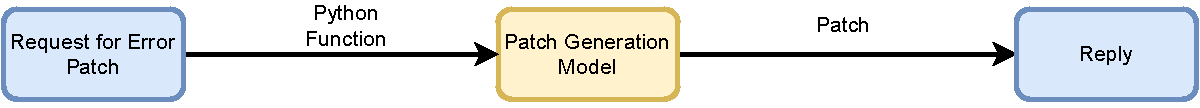
\includegraphics[width=1\textwidth]{obrazky-figures/error-correction-wizzrard.pdf}
       \caption{Block diagram of the Error Correction module using the Wizard model.}
      \label{fig:error-correction-wizzard}
    \end{figure}
%%%%%%%%%%%%%%%%%%%%%%%%%%%%%%%%%%%%%%%%%%%%%%%%%%%%%%%%%%%%%%
%% ###                                                        
%%  #  #    # #####  #      ###### #    # ###### #    # ##### 
%%  #  ##  ## #    # #      #      ##  ## #      ##   #   #   
%%  #  # ## # #    # #      #####  # ## # #####  # #  #   #   
%%  #  #    # #####  #      #      #    # #      #  # #   #   
%%  #  #    # #      #      #      #    # #      #   ##   #   
%% ### #    # #      ###### ###### #    # ###### #    #   #   
%%%%%%%%%%%%%%%%%%%%%%%%%%%%%%%%%%%%%%%%%%%%%%%%%%%%%%%%%%%%%%

\chapter{Implementation Details}
    The implementation of CodeImprove can be split into three parts. First, the training and experimentation software is implemented as a collection of Python and shell scripts. The server is also implemented in Python and uses some of the training infrastructure. Lastly, the client extension follows the standard format for Code extensions and is implemented in JavaScript.
    
    \section{Training}
    In the CodeImprove project, the training process itself is facilitated by \texttt{train.py}, which begins by parsing command line arguments using the \texttt{parse\_args} function from the \\ \texttt{my\_params} module. Then, the model loads a tokenizer with the assistance of the aforementioned Transformers library. 

    \subsection{Loading the Model}
    
        Next, based on a given \texttt{mode} command-line parameter, the script selected a proper data formatting function. This is done to accommodate the various kinds of models CodeImprove uses. The preprocessing functions themselves are defined in the \texttt{dataset\_formators} module. Then, the script loads the pre-trained model, which can be either an LED or a QLoRA model. 
        
        \medskip
        
        With QLoRA, the script also ensures that only the LoRA layers are used for training. Since the LED models used in this work are converted from pre-trained Bart models \ref{led}, we need to differentiate between layers that are initialized from scratch and layers that already contain relevant knowledge. 
        
        To dynamically find which layers are inherited from the Bart architecture, the script loads an additional Bart model and compares their state dictionaries. After that, the Bart model is unloaded from memory.
    
    \subsection{Loading Data}
    
        Then, the training data is loaded. The entry point for this operation is the \texttt{load\_data} function from the \texttt{my\_data} module. This function takes the tokenizer, the formatting function, and the parsed command line parameters and loads data entries from a \texttt{jsonl} file.
        
        \medskip
        
        The JSON Lines or \texttt{jsonl} format is a widely utilized file type for storing structured data in a compact and efficient manner. This format employs a simple but effective strategy where each line of the file represents a valid JSON object. This enables the data to be conveniently loaded and parsed in chunks or as a stream, allowing for more efficient processing and retrieval of information. 
        
        Each JSON entry is remapped into a native Python object for ease of use. Then, with the help of the formatting function, the data is filtered and tokenized to create the raw training data. This process creates the input and output token list and also a global attention mask, which is used with the LED models.
        
        The input and output tokens are first converted to IDs and padded to a uniform length, which is set as a command-line argument. \texttt{End of line} tokens are then appended. Finally, the script converts the data from lists to PyTorch tensors, which can be fed directly into the model.
        
        Additionally, attention masks are made for both input and labels by substituting the \texttt{padding} token with \texttt{False} and placing \texttt{True} everywhere else.
        
        This information is once again held in a custom object before being transformed into a dictionary with field names that conform to the standard naming for each respective element that the Transformer library expects. These dictionaries are returned in the form of a list, which finishes the data loading and preprocessing steps.
        
        \subsection{Training}
        The Transformers library offers a universal system for training models, which powers CodeImprove's training. First, a \texttt{TrainingArguments} object is created. This object stores the configuration of the training process with parameters such as batch size, the number of training epochs, and so on. It is initialized with the supplied command-line parameters.

        As stated earlier, the LED has two types of layers: those initialized with noise and those based on a pre-trained checkpoint of a BART model. We want to take a more aggressive approach during the training with the newly initialized layers and then with the pre-trained layers, as the gradients from the noisy layers could destroy the pre-trained knowledge.
        
        Because of this, a custom optimizer has been created. It accepts a learning rate for each of the two groups of layers. The reference code for this simplified optimizer was taken from one of the example scripts and modified to allow for the second learning rate.
        
        Layer freezing is another mechanism \texttt{train.py} uses to prevent the destruction of pre-trained knowledge. The pre-trained layers can be frozen for a configurable amount of training time. The eventual unfreezing is implemented via a \texttt{TrainerCallback}, and similarly, another call back is implemented that logs the values training statistics.
        
        Finally, the training begins, enclosed in a try-except that gracefully saves the model in case of an error or an interrupt signal.
        
        After the training, the model is saved to a file along with logged training information.

        \subsection{Training Configuration}

        For the LED models, the learning rate of $1 \times 10^{-5}$ for parameters inherited from PLBART and $3 \times 10^{-5}$ for newly initialized LED parameters proved to yield the best results. PLBART layers are also kept frozen for the duration of the first epoch. Warm-up steps, the number of steps during which the effective learning rate linearly moves from zero to the target learning rate, proved best when set in the lower thousands; for the final models, I have used the value of $1500$. A relatively high weight decay of $0.001$ worked well for preventing overfitting. The LED models took three iterations of the full CodeXGLUE code-to-text dataset to reach the point of underfitting.

    %%   ____ _ _            _   
    %%  / ___| (_) ___ _ __ | |_ 
    %% | |   | | |/ _ \ '_ \| __|
    %% | |___| | |  __/ | | | |_ 
    %%  \____|_|_|\___|_| |_|\__|
    \section{Client}
        In this case, the client is the Code extension. The extension focuses on providing quick and easy-to-use refactoring tools. 
        
        The extension makes use of Code's CodeLens API, which allows for rendering clickable text above chosen lines. The disadvantage of CodeLenses is that it creates spaces between the lines of code and moves the document. However, this only happens once when the extension is loaded, so the user should not feel major disturbances in their work.
        
        \medskip 
        
        CodeImprove uses these Code's \emph{DocumentSymbolProvider}, an API for generic programming language parsing, to obtain the list of all functions and methods in the document and uses it to display the options to scan the body of the code for Bugs and an option to generate new comments. 
        
        The extension also monitors changes in text selection, and when the user puts their cursor over variable declarations, it offers the name suggestion action.
        
        %% image of function and its CondeLense options
        \begin{figure}[ht!]
          \centering
          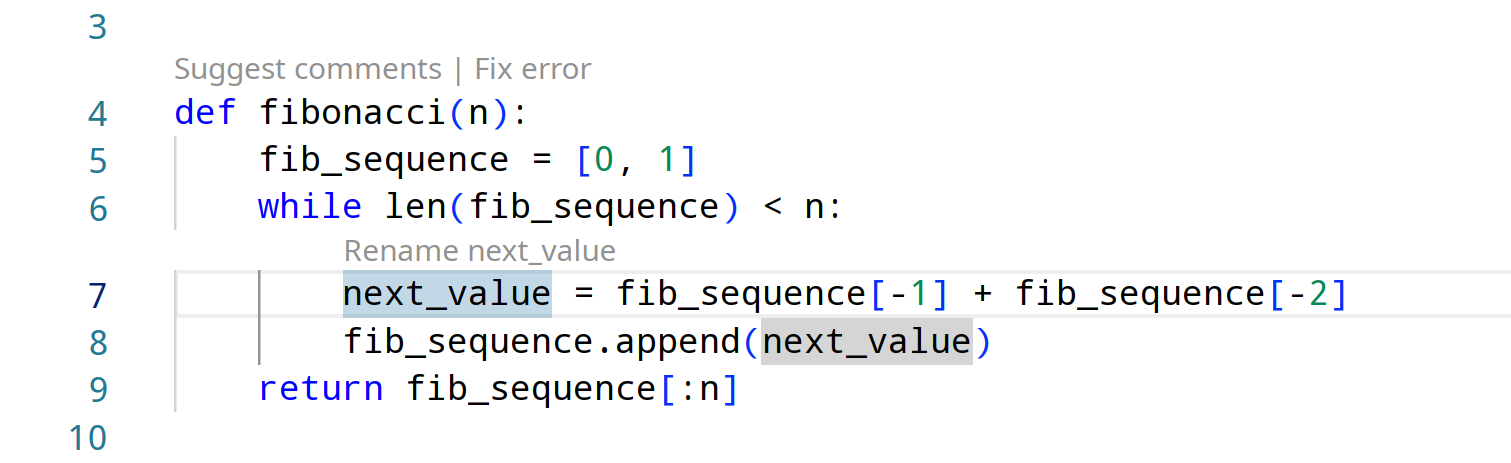
\includegraphics[width=\textwidth]{obrazky-figures/vscode-function.png}
          \caption{CodeLens options appearing around in a function, showing three clickable labels in total. The first two appear above the function definition, "Suggest comments" opens a panel with suggestions for extra code comments, and "Fix error" analyzes code for potential errors and offers a solution. The third appears on line 7 and reads, "Rename next\_value." Clicking it opens a variable name suggestion panel. This option is only shown because the user moved their text cursor over the variable name.}
          \label{fig:vscode_function}
        \end{figure}
        
        When the user clicks on any of these CodeLenses, a temporary side panel will open and display a loading screen while the extension sends a request to the server and, upon getting a response, displays it. The address and port of the server can be specified in the settings.
        
        \subsection{Comment Generation}
            The comment generation panel lets you change the docstring convention between no formatting, Google, NumPy, and reStructuredText. Underneath is a code view that displays how the function will look after the changes are applied. All comments stand alone on their own line. The docstring will be generated only if it was previously missing. Inserted lines appear highlighted in the code view. See figure \ref{fig:vscode_comments}.
        
        \begin{figure}[ht!]
          \centering
          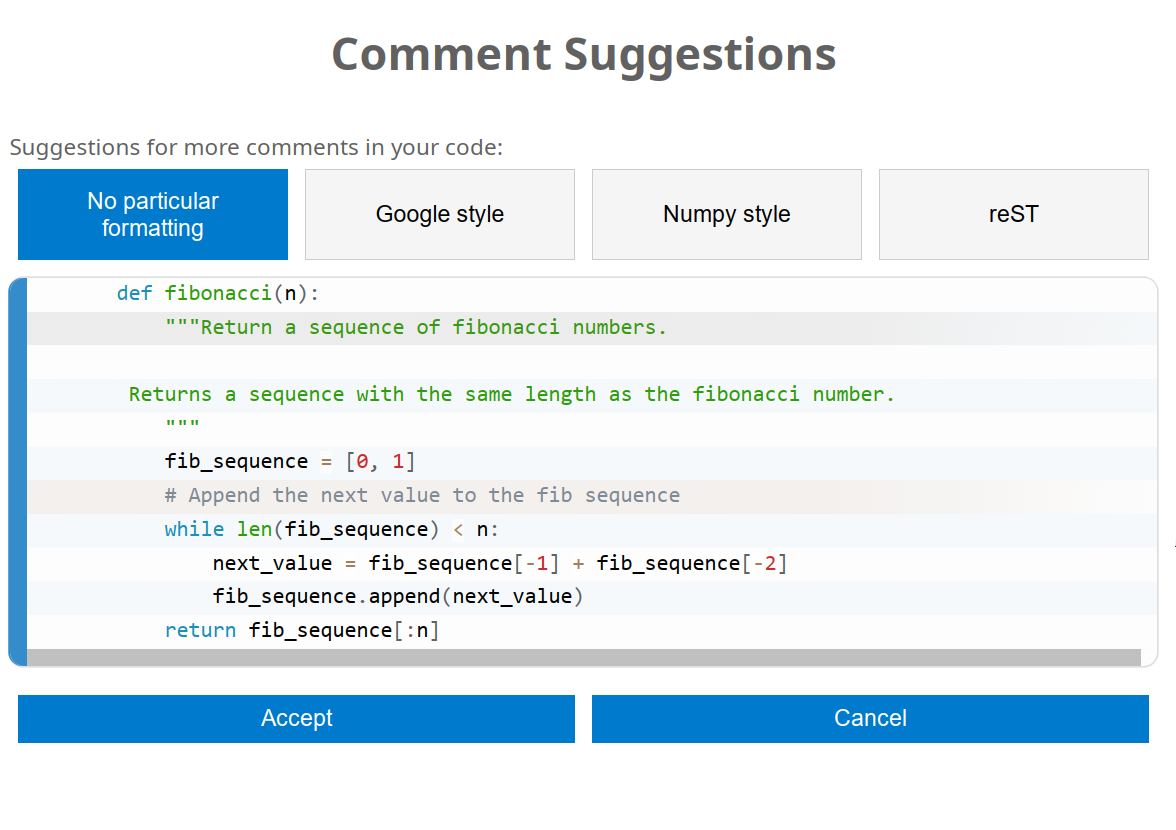
\includegraphics[width=0.8\textwidth]{obrazky-figures/CodeImprove-comment-screenshot.png}
          \caption{CodeImprove comment suggestion window. It is currently suggesting a new docstring and a comment above the while loop.}
          \label{fig:vscode_comments}
        \end{figure}
        
        \subsection{Error Correction}
            The error correction panel similarly uses a code view to display the suggested change, but this time, the data is displayed more like a traditional \emph{diff} view. Inserted lines are highlighted with a lighter color, and deleted lines with a darker color. Each line is annotated with a comment \texttt{New}, \texttt{Removed} for inversion and deletion, respectively, and \texttt{Before} and \texttt{After} for substituting the original line of text. These comments are only visible in this preview panel and won't be present in the code when the changes are applied. See figure \ref{fig:vscode_errors}.
        
        \begin{figure}[ht!]
          \centering
          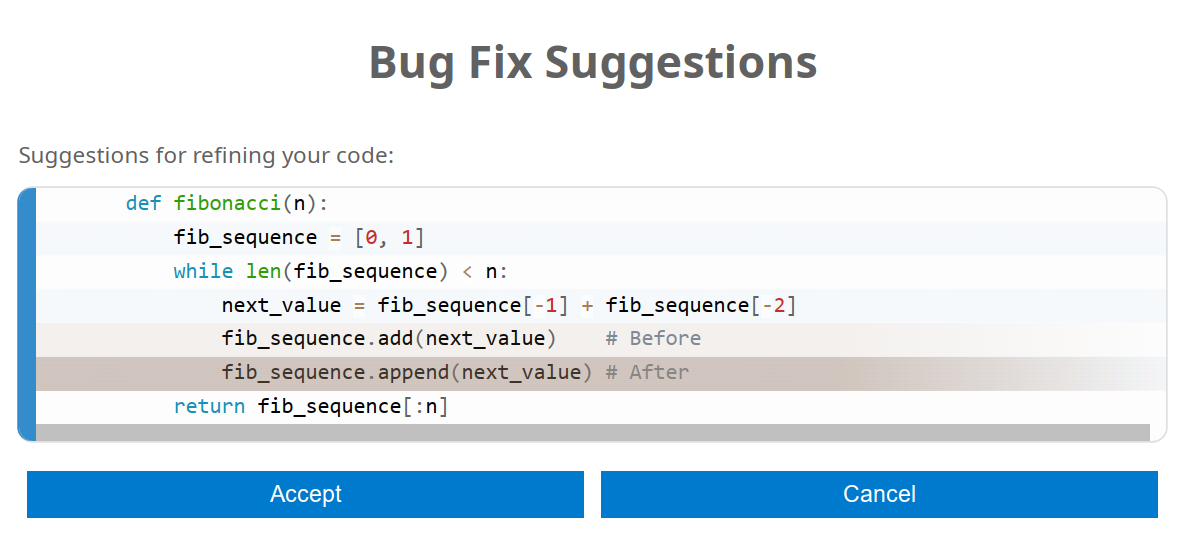
\includegraphics[width=0.85\textwidth]{obrazky-figures/codeimprove-bugfix.png}
          \caption{CodeImprove suggestion for error correction, changes are highlighted. Note that this suggestion was mocked.}
          \label{fig:vscode_errors}
        \end{figure}
        
        \subsection{Variable name suggestion}
            The renaming panel presents the user with three choices for a variable name, which the user selects by clicking on them. See figure \ref{fig:vscode_rename}.
        
        %% Rename screen
        \begin{figure}[ht!]
          \centering
          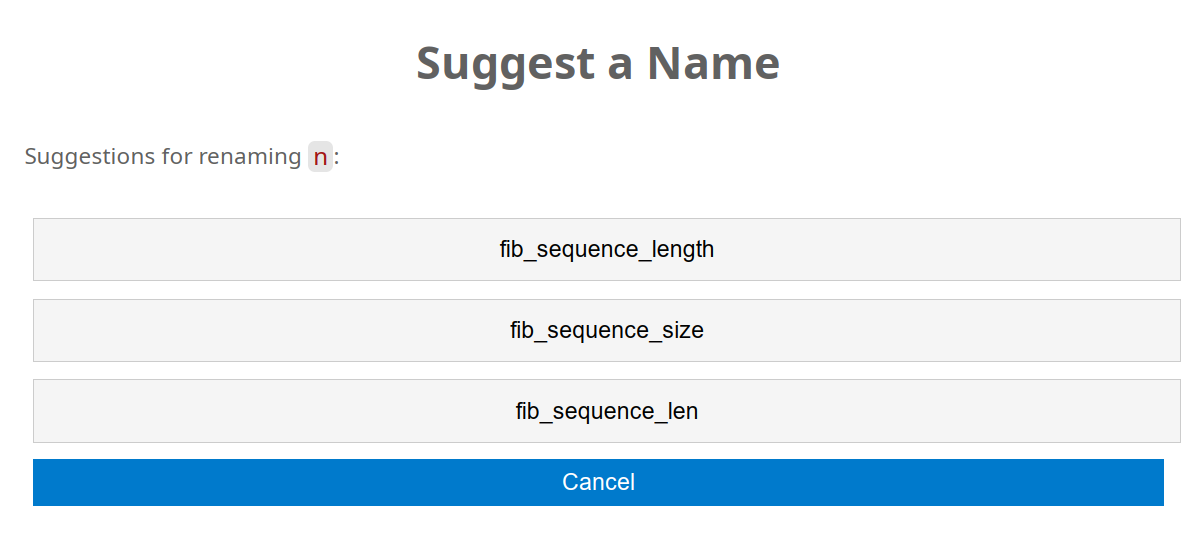
\includegraphics[width=0.85\textwidth]{obrazky-figures/codeimprove-rename.png}
          \caption{CodeImprove suggestion for an alternative variable name.}
          \label{fig:vscode_rename}
        \end{figure}
        
        \subsection{Scope of Functionality}
            CodeImprove operates only on functions and methods. Code that is not inside any of those code blocks cannot be evaluated; this decision stems from the Datasets and the ease of training. Functions provide a mostly closed-off window to code with a singular purpose; working with larger chunks of code would require high input length, introduce a lot of noise into the training, and require much larger models to evaluate.
        
            Likewise, code inside a function that is itself inside another function cannot be evaluated independently from its parent function, though this practice seems to be used only rarely in Python.
            
            The client receives instructions on what to change and composes the post-change code accordingly. The only exception is renaming, which has to have its post-change generated on the server side because Code does not expose any APIs for renaming identifiers, even though this functionality is available in the editor as a GUI feature. The only available option similar to this is \texttt{editor.action.rename}, which does not accept the new name and will only open the renaming dialog to the user. Hence, the choice of processing on the server came naturally after this, as Free JavaScript libraries do not offer the same level of quality when parsing Python code as Python's standard library.
            
    \section{Server}
        The server side is implemented in \texttt{server.py}, allowing users to run inferences on their code. It is controlled by a TOML configuration file, which specifies paths to each model and the configuration for running inference on them. The configuration file also includes a port on which the application communicates; by default, this is set to 8182.
        
        The server uses an event loop to wait for incoming requests. Upon a request, \texttt{server.py} will parse the request, select the appropriate model, and use the code formatting functions from \texttt{dataset\_formators} that are used for training, and in the case of LED models, it even calls the PLBART preprocessing function, to make sure that the data is presented to the model in a familiar form. 

        Responses are formatted into a JavaScript object and serialized as JSON before being sent back to the user.
        
\subsection{Communication}
    The client and the server exchange information via the HTTP protocol. The communication is completely stateless and uses the traditional request-response format. The client always initiates it via a \texttt{POST} request containing a JSON-encoded payload with structured information, such as the type of suggestion that is being requested and the snippet of the function code, see listing \ref{lst:request} for more details about the format of requests and listing \ref{lst:response} for responses.  
    
\capstartfalse
\begin{figure}[H]
  \begin{lstlisting}[caption={The request message data structure. \texttt{uuid} is meant for identification of the message, \texttt{requests} is a list of individual requests, identified with \texttt{id}, which is a serial number of the request, \texttt{snippet} contains the code snippet this request applies to and \texttt{tasks} is a list of task objects, each contains its task type in \texttt{task}, which is either "rename" for the suggestion alternative names to variables, \texttt{error} for fixing errors and \texttt{comment} for inserting additional comments. The field \texttt{symbol} is present only in \texttt{rename} tasks used to specify the name of the variable for renaming, and \texttt{style} is similarly only present in \texttt{comment} tasks and specifies the docstring preference.}, label={lst:request}, numbers=none]
Request Message {
    uuid: string
    requests: [
        {
            id: integer
            snippet: string
            tasks: [
                {
                    task: "rename" | "error" | "comment"
                    symbol: string (when task = "rename")
                    style: "NA" | "GO" | "NP" | "RE" (when task = "comment")
                }
            ]
        }
    ]
}\end{lstlisting}
  \centering
  \begin{lstlisting}[caption={The response message data structure. \texttt{uuid} matches the \texttt{uuid} of the request. \texttt{response} is a list of the individual responses. \texttt{id} and \texttt{task} together match up with their respective field in the request and serve to identify the response. \texttt{status} is meant to signify the result of the task. \texttt{result} contains the output of the task; for comment generation and error correction, this is a string; however, for the renaming task, this is a list where each element represents one rename suggestion and contains both the new name for the variable and the code snippet with the substituted name.}, label={lst:response}, numbers=none]
Response Message {
    uuid: string
    response: [
        {
            id: integer
            tasks: "rename" | "error" | "comment"
            status: "ok" | "error"
            result: string | list
            ]
        }
    ]
}
  \end{lstlisting}
\end{figure}

%%%%%%%%%%%%%%%%%%%%%%%%%%%%%%%
%% #######                      
%% #       #    #   ##   #      
%% #       #    #  #  #  #      
%% #####   #    # #    # #      
%% #       #    # ###### #      
%% #        #  #  #    # #      
%% #######   ##   #    # ######
%%%%%%%%%%%%%%%%%%%%%%%%%%%%%%%
\chapter{Evaluation and Results}
    Finally, CodeImprove's models need to be tested against the competition in order to judge their performance and usability.  GPT-3.5-turbo by OpenAI was chosen as the baseline for comparing performance since it is, from publicly available information, the closest model to the one used in GitHub copilot, or at least the closest that is publicly available.
    
    Each benchmark was computed from a thousand samples that CodeImprove has not seen during training; sadly, due to the nature of large-scale data collection OpenAI employs, it is impossible to verify that the same applies to the GPT-3.5-turbo model.
    
    \section{Assessment of Comment Generation}
        \subsection{\textsc{Bleu}}
        \textsc{Bleu} (Bilingual Evaluation Understudy) is a metric introduced by\,\cite{papineni-etal-2002-bleu}; it stands as one of the most prominent automated methods used for quantifying similarity between two pieces of text. \textsc{Bleu} evaluates the quality of machine-generated text by calculating the correspondence between it and a set of high-quality reference outputs. \textsc{Bleu} was originally developed to track the performance of translators, but it will serve us well when rating the similarity of a reference comment to one generated by our system.
        
        The goal of \textsc{Bleu} is to quantify similarity while allowing for changed word order or a partially different choice of words. Despite being based on a simple algorithm, \textsc{Bleu} was found to rate translations similarly to human reviewers.
        
        At its core, \textsc{Bleu} works by counting how many correct words (unigrams) from the prediction appear in the reference output, divided by the number of words in the prediction. The presence of a word only counts up to the number of occurrences of that particular word in the reference output. 
        The same is also done with sequences of two words (bigrams), three words (trigrams), and four words (guadgrams). The longer the measured sequence is, the lower the score will be in practice. To balance this, the scores are averaged with a geometric mean.
        
        Lastly, \textsc{Bleu} penalizes sentences that are shorter than the shortest reference translation with multiplayer.
    
        \begin{equation}
            BP = 
            \begin{cases} 
                1 & \text{if } c > r \\
                e^{(1-r/c)} & \text{if } c \leq r 
            \end{cases}
        \end{equation}
        Where $c$ is the number of words in the candidate, and $r$ is the number of words in the reference. 
        
        The full equation is a s follows:
        \begin{equation}
            \text{\textsc{Bleu}} = BP \times \exp\left(\sum_{n=1}^{N} w_n \log p_n\right)
        \end{equation}
        Where BP is the brevity penalty, $ p_n$ is the number of n-grams from the prediction that matches the reference. $w_n$ are weights assigned to each n-gram; typically,y these are 1/n. N is the size of the largest n-gram 
            
    \subsection{Inline Comment Generation}

    Machine evaluation suggests that CodeImprove-comment outperforms GPT-3.5-turbo by nearly three points, as shown in table \ref{tab:comment_perf}. Even though the baseline dominates unigram precision, CodeImprove-comment outperforms it in bigram predictions as well as trigram predictions, where GPT-3.5-turbo severely lags behind. Neither model does very well in quadgram predictions, but CodeImprove-comment retained a slight lead. The baseline results were collected using the prompt in listing \ref{lst:comment_prompt}.
    
    \begin{table}[H]
        \centering
        \begin{tabular}{|c||c|c|c|c|c|}
        \hline
         & \textsc{Bleu} total & Unigram & Bigram & Trigram & Quadgram \\
        \hline
        \hline
        CodeImprove-comment & \textbf{14.99\,\%} & 72.7\,\% & \textbf{40.0\,\%} & \textbf{5.6\,\%} & \textbf{3.1\,\%} \\
        \hline
        GPT-3.5-turbo & 12.04\,\% & \textbf{94.1\,\%} & 37.5\,\%, & 3.3\,\% & 1.8\,\% \\
        \hline
        \end{tabular}
        \caption{\textsc{Bleu} score comparison between CodeImprove-comment and GPT-3.5-turbo in inline comment generation on one thousand samples. All ngrams are weighed equally.}
        \label{tab:comment_perf}
    \end{table}
    
    \begin{lstlisting}[caption={Prompt used for sampling docstrings from GPT-3.5-turbo.}, label={lst:comment_prompt}, numbers=none]
ASSISTANT:
    I am an AI for generating inline code comments. Please add a marker of where you would like me to add a comment. I will not generate a short comment relevant to that part of the code and the particular line, I respond with nothing but the text content of the generated comment and will not contain any surrounding code or even the # symbol. I can be used as an API.
USER:
    < code with one line marked for commenting >
    \end{lstlisting}

    Upon human evaluation, it becomes obvious that GPT-3.5-turbo has much better performance. CodeImprove-comment sometimes produces almost nonsensical outputs, though other times, it is able to generate intelligent and insightful comments. However, the baseline model is much more consistent in producing its quality, and its inaccuracies seem to stem from the fact that the model decided to describe the situation in a different way. See examples of CodeImprove-comment's output in \ref{comment_pred}.

    Overall, the CodeImprove-comment model is only able to surpass the baseline in \textsc{Bleu} evaluation but ultimately underperforms in the eyes of a human review.
    
    \subsection{Docstring Generation}
    As seen in table \ref{tab:docstring_perf}, CodeImprove-docstring is not able to break past the baseline, which dominates precision in almost every engram category except for quadgram, where neither model did particularly well, and GPT-3.5-turbo fell behind by almost a percentage point.
    
        \begin{table}[H]
            \centering
            \begin{tabular}{|c||c|c|c|c|c|}
            \hline
             & \textsc{Bleu} total & Unigram & Bigram & Trigram & Quadgram \\
            \hline
            \hline
            CodeImprove-docstring & 27.92\,\% & 67.6\,\% & 42.4\,\% & 21.9\,\% & \textbf{9.7\,\%} \\
            \hline
            GPT-3.5-turbo & \textbf{38.01}\,\% & \textbf{98.3\,\%} & \textbf{78.0\,\%}, & \textbf{31.0\,\%} & 8.8\,\% \\
            \hline
            \end{tabular}
            \caption{\textsc{Bleu} score comparison between CodeImprove-docstring and GPT-3.5-turbo in docstring generation on one thousand samples. All ngrams are weighed equally.}
            \label{tab:docstring_perf}
        \end{table}

    \begin{lstlisting}[caption={Prompt used for sampling inline comment from GPT-3.5-turbo.}, label={lst:docstring_prompt}, numbers=none]
ASSISTANT:
    I am an AI for generating docstrings for Python 3 code. You need to prepend your code with "$ DOCSTR code$" where "code" specifies which docstring convention you want me to generate. "NP": NumPy docstring, "GO": Google docstring, "RE": for reST docstring and "NA": for other/no formatting. I will output a fitting docstring describing the code you gave me. My outputs only contain the docstring text content. I can be used as an API.
USER:
    < code >
    \end{lstlisting}

    As figures \ref{fig:docstring_length_gpt} and \ref{fig:docstring_length_codeimporove} show, there is an observable downward trend in accuracy as the character count increases.

    GPT-3.5-turbo manages to retain more accuracy as its score decreases linearly with increasing character count; on the other hand, CodeImprove-docstring loses precision with a slight exponential curve.

    Both models lose all accuracy beyond the 7000-character mark.

    \begin{figure}[H]
      \centering
      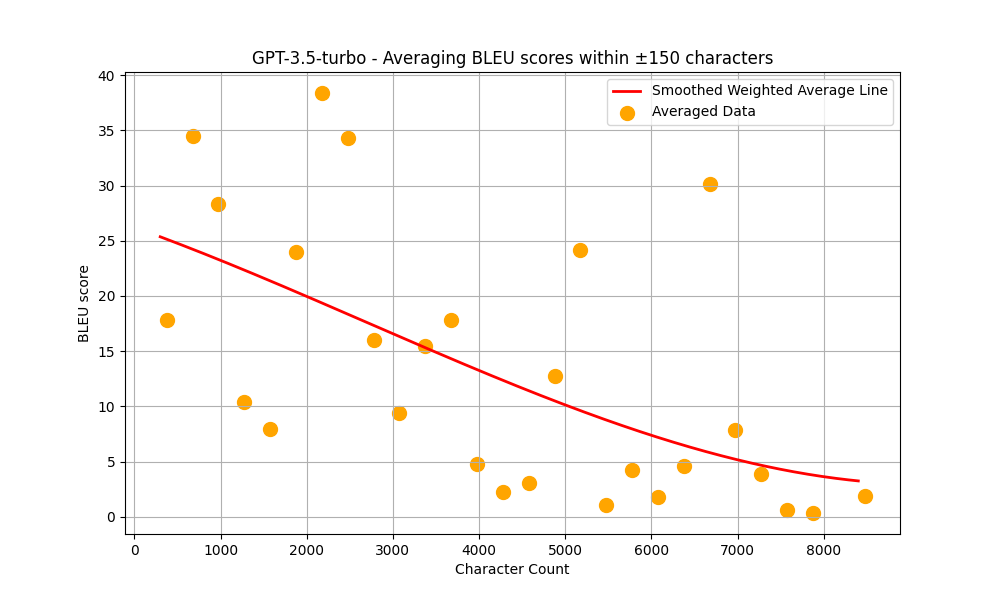
\includegraphics[width=0.95\textwidth]{obrazky-figures/docstring-gpt-bleu.png}
       \caption{\textsc{Bleu} score over character length of the input of GPT-3.5-turbo while generating docstrings.}
      \label{fig:docstring_length_gpt}
    \end{figure}

    \begin{figure}[H]
      \centering
      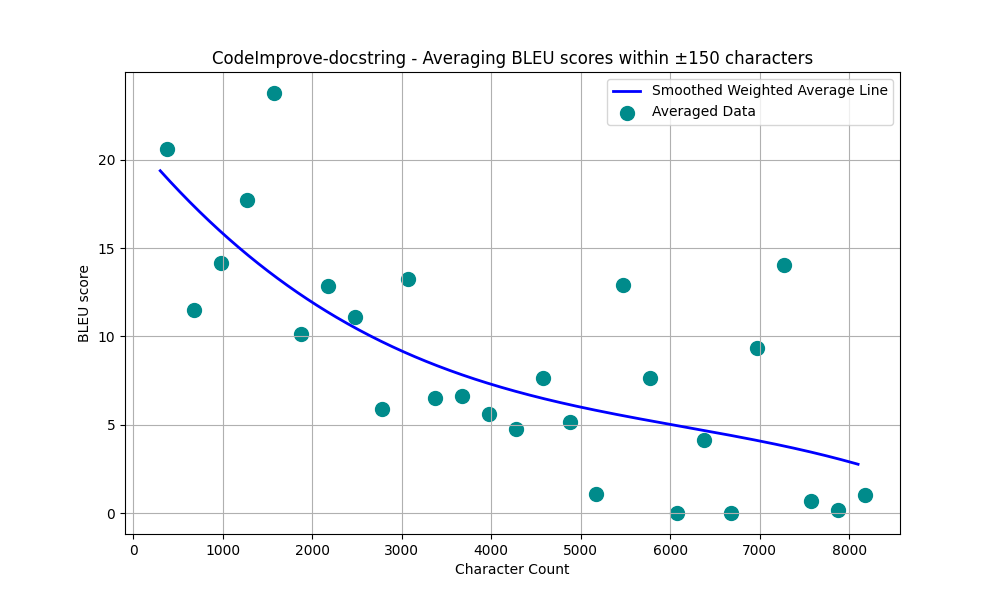
\includegraphics[width=0.95\textwidth]{obrazky-figures/Ncodeimprove-docstring.png}
       \caption{\textsc{Bleu} score over character length of the input of the CodeImprove-docstring model.}
      \label{fig:docstring_length_codeimporove}
    \end{figure}
    
    Upon human inspection, it is apparent that the quality of the docstring is much lower than the baseline. CodeImprove's docstrings are noticeably shorter than the labels.

    It is apparent that CodeImprove makes an effort to describe functions of individual parameters; however, it often fails to name them all. The model also appears to struggle with following the ordered docstring notation.

    Overall, this model does not manage to outperform the baseline either in terms of algorithmic or human evaluations.

    See examples of predictions in appendix \ref{docstr_pred}.
    
    \section{Assessment of Variable Name Generation}
    \subsection{Top3 Unigram Precision}
        Measuring the performance of variable name suggestions is somewhat nuanced. Variable names consist of several keywords, often with arbitrary word ordering.
    
        In order to take this into account when benchmarking this module, a custom variant of the traditional precision metric, dubbed \emph{Top3 Unigram precision (T3UP)}, is used. At its core, it is a ratio of the number of exact matches of unigrams $m$ between the prediction $u$ and the reference $r$ divided by either the length of the reference or the length of the prediction, whichever is greater. This way, three scores are computed from three separate predictions, and the highest one is used as the final TOP3 Unigram Precision.
        
        \begin{equation}
        \text{TOP3UP} = \max_{i=1}^{3} \left(\frac{m_i}{\max\left(\textit{length}(r), \textit{ length}(p_i)\right)}\right) \times 100
        \end{equation}
        
        The rationale for using 3 predictions to calculate the metric is that the CodeImprove extension presents the user with three choices.
        
        This approach, although simple, fits well with the nature of variable name composition, which is itself relatively primitive.

        Variable names are segmented by splitting on the boundary of a lowercase and uppercase letter to cover the camel case. A split is also performed where letters meet digits, and lastly, underscores cause a split as well to cover the snake case.

    \subsection{Performance}
        As we can see in table \ref{fig:rename_perf}, CodeImprove slightly underperformed compared to the baseline model. 
        
        \begin{table}[H]
            \centering
            \begin{tabular}{|c||c|c|}
            \hline
             & CodeImprove-rename & GPT-3.5-turbo \\
            \hline
            \hline
            TOP3UP & 35.63\,\% & \textbf{37.74\,\%} \\
            \hline
            TOP3EM & 10\,\% & \textbf{18\,\%} \\
            \hline
            \end{tabular}
            \caption{\emph{TOP3UP} is Top3 Unigram Precision, and \emph{TOP3EM} is a percentage of exact matches from 3 generated results.}
            \label{fig:rename_perf}
        \end{table}

        Results from the baseline model were extracted with a prompt specified in listing \ref{lst:rename_prompt}.
        
        \begin{lstlisting}[caption={Prompt used for sampling variable names from GPT-3.5-turbo.}, label={lst:rename_prompt}, numbers=none]
ASSISTANT:
    I am a system for generating variable names. I will accept a snippet of Python code with "<mask>" as a replacement for one of the variable names. All mask tokens hide the same variable name. I will respond with three different suggestions for what the name should be. I will consider the context of the code they are found in to generate the most accurate results. I will separate the three variable names with a comma, My output will not contain anything else but the variable names.
USER:
    < code with masked variable name >
        \end{lstlisting}

        Both models in figures \ref{fig:rename_length_gpt} and \ref{fig:rename_length_codeimporove} (note that they have different scales) show a similar curve that rises and peaks at around 2300 characters and then drops off. GPT-3.5-turbo experiences a relatively sharp drop-off, whereas CodeImprove-rename manages to retain accuracy far better and, in spite of the rising character count, only loses score linearly and quite mildly.
        
        The rise could be caused by more useful information to infer the purpose of the variable. The drop-off at higher character counts may be due to longer functions being more complex and obscure, making it more difficult to determine the purpose of individual variables.

        \begin{figure}[H]
          \centering
          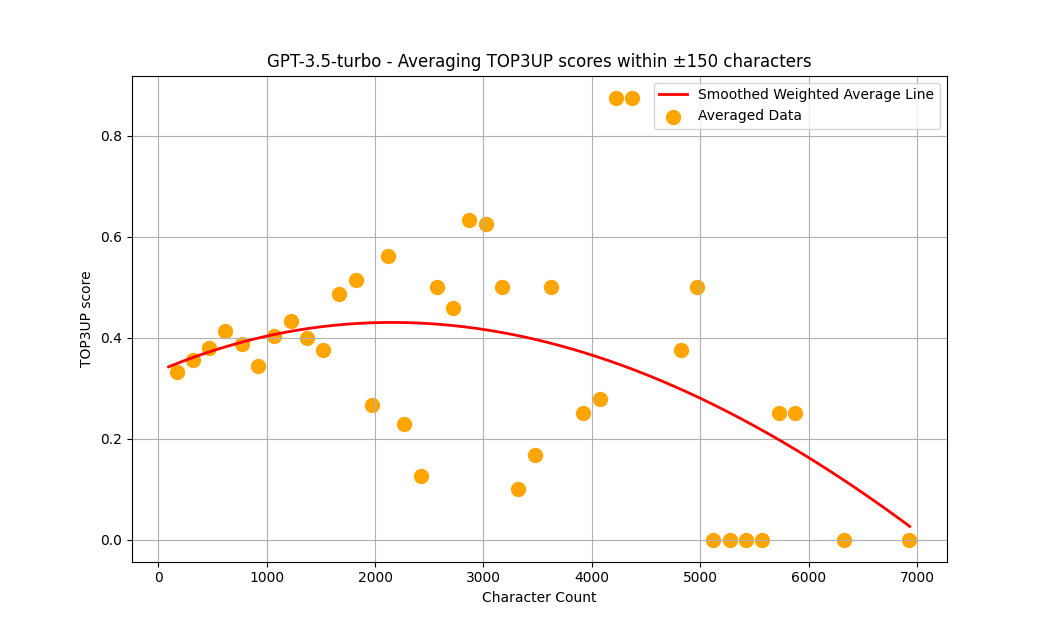
\includegraphics[width=0.85\textwidth]{obrazky-figures/gpt3turbo-rename-average.png}
           \caption{TOP3UP score over character length of the input of GPT-3.5-turbo.}
          \label{fig:rename_length_gpt}
        \end{figure}
        \begin{figure}[H]
          \centering
          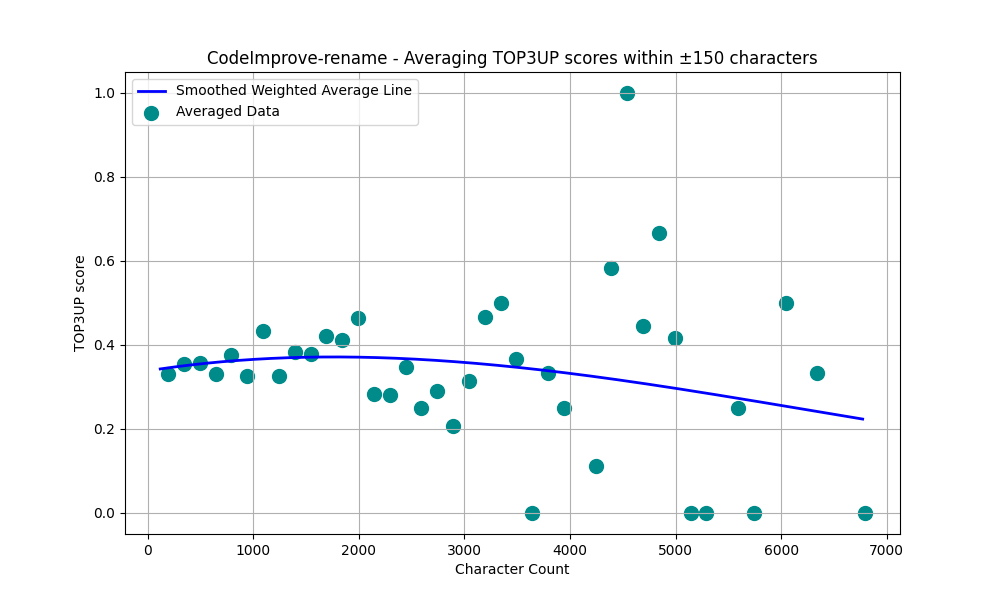
\includegraphics[width=0.85\textwidth]{obrazky-figures/codeImprove-rename-average.png}
           \caption{TOP3UP score over character length of the input of CodeImprove-rename.}
          \label{fig:rename_length_codeimporove}
        \end{figure}

        Overall, CodeImprove-rename outperforms GPT-3.5-turbo on long inputs but falls behind on shorter inputs.

        See appendix \ref{rename_pred} for examples of predictions.
        
    \section{Assessment of Error Correction}
        \subsection{LED approach}
        As mentioned in an earlier section, the LED approach to error detection proved ineffective, just from the results of the detection model; see a summary of its performance \ref{tab:error_detection}.
        \begin{table}[H]
            \centering
            \begin{tabular}{|c|c|}
            \hline
            \textbf{Error type} & \textbf{Number of samples}  \\
            \hline
            Correctly identified & 188 \\
            Incorrectly identified & 812 \\
            \hline
            \hline
            \textbf{Error lines} & \textbf{Number of samples}  \\
            \hline
            Correctly correct & 22 \\
            Partially correct & 353 \\
            All incorrect\ & 625 \\
            \hline
            \hline
            \textbf{Error presence} & \textbf{Number of samples}  \\
            \hline
            Correctly identified as \textit{no errors} & 153 \\
            Incorrectly identified as \textit{no errors} & 847 \\
            Incorrectly identified as \textit{has errors} & 863 \\
            \hline
            \end{tabular}
            \caption{Performance of the LED-based Error Detection model.}
            \label{tab:error_detection}
        \end{table}

        From closer inspection of the results, the model seems to be trying to learn the average distribution of erroneous lines, often guessing numbers in the lower ranges, which it probably learned to be a safe bet from shorter samples. However, the model does make predictions in the higher ranges as well and usually outputs numbers in the correct order. It mostly does not cross the number of the last line, though there are examples where it does.

        When it comes to detecting types of errors, the model performs similarly poorly. Most often guessing \texttt{TypeError}, though it often predicts others as well.

        In order to increase the chances of success, other approaches were modifications to the dataset explored, including variants that only included erroneous code with no false positives and only using the name of the exception class from the PyTraceBugs dataset as the error type, but the results remained similarly unsatisfactory.

        It is clear that the LED model for error detection, despite great efforts, fails to grasp the nuances of the task at hand.

        \subsection{CodeWizard approach}

        QLoRA adaptation was utilized to train the instruction-tuned CodeWizard to perform both patch-based and full code error correction. Sadly, training the LoRA layers did not yield fruits, as the model kept failing to converge even after exploring various combinations of adapter parameters. 

    
\chapter{Conclusion}
    This thesis addresses the development of a Visual Studio Code extension called CodeImprovem. The extension specifically targets the automation of comments and docstrings generation, offers suggestions for alternative variable names, and incorporates an error correction feature. It operates on function and method bodies, aiding programmers in maintaining and improving the quality and readability of their codebases.

    This work covers the basic theory and state-of-the-art practices in natural language processing. It also examines a sparse attention transformer model architecture called Longformer, which allows for the efficient processing of large sequences of code. Quantized low-rank adaptation is also explored to correct erroneous code.
    
    The extension introduced in this thesis facilitates the generation of context-specific comments and docstring, striving to help developers improve the readability of their code. It is powered by a pair of Longformer models. The suggestion of variable names is also powered by its own Longformer model. This feature aims to assist developers, particularly those who struggle creatively with naming variables. Additionally, as part of this work, a dataset containing over 16,500 samples of errors before and after patches was amassed. Despite initial attempts to implement error correction with Longformer and subsequent trials with the CodeWizard model enhanced by QLoRA, neither approach achieved the desired outcomes, producing irrelevant outputs. 
    
    The models were compared to GPT-3.5-turbo, which is a similar model used in GitHub copilot, a leading chat-based programming assistant. The docstring generator scored about 27\,\% lower \textsc{Bleu} compared to the baseline, the model for generating inline comments outperformed the baseline by about 20\,\% in \textsc{Bleu} score. The model for variable name suggestion scored about 6\,\% worse in TOP3 Unigram Precision.

    However, upon human evaluation, all three models showed results that were significantly poorer than the baseline.
    
    This work strives to create an integrated toolset that will seamlessly integrate modern advancements in machine learning into the UI and enable frictionless use of simple AI-aided tasks for operations that need to be performed most often, without the need to deal with prompts and chat windows. This goal was partially reached, leaving a lot of room for improvement. Further development should focus on including more user preference options and could use QLoRA adaptation with a larger model, which would fine-tuned multimodally and facilitate all functionality. Adding additional features would also strengthen the experience.

  \else
    % Tento soubor nahraďte vlastním souborem s obsahem práce.
%=========================================================================
% Autoři: Michal Bidlo, Bohuslav Křena, Jaroslav Dytrych, Petr Veigend a Adam Herout 2019

% Pro kompilaci po částech (viz projekt.tex), nutno odkomentovat a upravit
%\documentclass[../projekt.tex]{subfiles}
%\begin{document}

\chapter{Úvod}

Tento text slouží jako ukázkový obsah šablony a současně rekapituluje nejdůležitější informace z předpisů a poskytuje další užitečné informace, které budete potřebovat pro tvorbu technické zprávy ke svojí práci. Než se šablonou budete dále pracovat, je třeba vědět, jak ji správně použít. To je stručně uvedeno v~příloze \ref{jak}.

I když některým studentům pro napsání dobré diplomové práce (bakalářská práce je také diplomová -- dostává se za ni diplom) stačí znát a dodržovat oficiální formální požadavky uvedené ve směrnicích a typografické zásady, často je výhodné před započetím psaní zjistit, jaké jsou osvědčené postupy pro psaní odborného textu a jak si práci usnadnit. Někteří vedoucí svým studentům připravili popisy osvědčených postupů, které vedly k desítkám úspěšně obhájených prací. Výběr nejzajímavějších postupů, které měli autoři této šablony k~dispozici ve chvíli její tvorby, je v níže uvedených kapitolách. Má-li Váš vedoucí svoji stránku s doporučenými postupy, tyto kapitoly můžete vynechat a řídit se pokyny svého vedoucího. Pokud takovou stránku nemá, může být přečtení níže uvedeného textu vhodnou přípravou na konzultaci o plánované struktuře a náplni textu práce.

Diplomová práce je rozsáhlé dílo a tomu odpovídá i technická zpráva. Ne každý je schopen si sednout a jednoduše ji napsat. Je třeba vědět, kde začít a jak postupovat. Jedním z možných přístupů je začít psaním klíčových slov a abstraktu, abyste si ujasnili, co je v~práci nejdůležitější. O tom pojednává kapitola \ref{abstrakt}.

Po sepsání abstraktu se lze pustit do psaní samotného textu technické zprávy. Typicky si nejprve připravíme základní strukturu práce, kterou pak budeme plnit textem. Kapitola \ref{struktura} se zabývá základními informacemi a radami pro psaní odborného textu, které Vám pomohou vyhnout se začátečnickým chybám, a stanovením nadpisů kapitol a přibližných rozsahů jednotlivých částí práce. V závěru kapitoly je pak uveden přístup, kterým si lze psaní technické zprávy značně usnadnit.

Diplomové práce v oblasti informačních technologií mají určitou typickou strukturu. Po~úvodu bude následovat kapitola či kapitoly zabývající se shrnutím současného stavu, který bude v následujících kapitolách zhodnocen a bude navrženo řešení, které bude implementováno a otestováno. V závěru pak budou výsledky vyhodnoceny a bude navržen budoucí vývoj. I když se názvy a rozsahy kapitol v různých pracích liší, vždy tam lze najít kapitoly odpovídající této struktuře. Kapitola \ref{kapitoly} se zabývá obsahy typických kapitol, které se v diplomových pracích z oblasti IT vyskytují. Většina studentů ve svojí práci pravděpodobně využije pouze určitou podmnožinu popsaných kapitol, která je pro jejich práci relevantní. Uvedené popisy a rady mohou pomoci jak s~rozhodnutím, zda danou kapitolu uvést, tak i~s~vnitřní strukturou a samotným obsahem kapitoly.

Za závěrečnou kapitolou práce vždy následuje seznam použité literatury. Citacemi, které tento seznam tvoří, a odkazy na ně se zabývá kapitola \ref{citace}. Byť to tak nezkušený student nemusí vnímat, je seznam použité literatury a odkazy na něj pro práci zcela zásadní. Hodnocení práce s literaturou a citací tvoří jednu z důležitých částí posudku oponenta a bude-li chybět jediná položka, může to vést k hodnocení stupněm F, následnému disciplinárnímu řízení za plagiátorství a k vyloučení z nedokončeného studia. Nesprávná práce se zdroji může mít i další důsledky -- v roce 2018 stála křesla dva členy české vlády. Proto prosím citacím věnujte odpovídající pozornost. 

Po dokončení textu je nutné zjistit, jaké požadavky jsou kladeny na vysokoškolskou kvalifikační práci na FIT VUT v~Brně, a dořešit případné nedostatky. Formální požadavky jsou uvedeny ve směrnicích a na webových stránkách, které jsou zmíněny v kapitole \ref{formality}. Tato kapitola obsahuje i požadované rozsahy jednotlivých typů prací a další vybrané informace z~předpisů a doporučení. V závěru kapitoly je uveden přehled nejčastějších chyb, se kterými se oponenti setkávají a kterým byste se měli vyhnout. Hodnocení formální úpravy práce je pak další z důležitých součástí posudku oponenta.

Po odstranění formálních nedostatků lze práci odevzdat. Před odevzdáním práce si můžete projít kontrolní seznam (tzv. \uv{checklist}) uvedený v příloze \ref{checklist}. Samotné odevzdání listinné i elektronické verze práce je pak popsáno v kapitole \ref{odevzdani}.

V závěrečné kapitole \ref{zaver} je pak uvedeno shrnutí toho, co se lze přečtením tohoto textu dozvědět, a to nejdůležitější, na co je třeba myslet před odevzdáním práce.


\chapter{Abstrakt}
\label{abstrakt}
Pod nadpisem Abstrakt je uvedeno shrnutí práce zabírající prostor maximálně 10 řádků. Z~dobrého abstraktu by mělo být i přes jeho malý rozsah patrné, jaký problém se řešil, jaký přístup k jeho řešení byl v práci použit a jakých výsledků bylo dosaženo. Účelem abstraktu je, aby potenciální čtenář práce již po přečtení abstraktu věděl, zda v práci najde to, co hledá \cite{fitWeb}. Zbytek této kapitoly byl převzat z blogu prof. Herouta \cite{Herout}.
\bigskip

\noindent Za prvé – na abstraktu záleží. Za druhé – není těžké ho napsat. Pojďme na to.

\subsection*{K čemu je abstrakt}
Abstrakt slouží k \bf vyhledávání\rm, společně s názvem dané vědecké práce a seznamem klíčových slov. Tyto části (snad s výjimkou názvu) nejsou přímo součástí textu a nečeká se, že někdo, kdo by zasedl ke čtení dané vědecké práce, bude číst je. To, že práci čte, znamená, že už se dostal za fázi čtení abstraktu. Abstrakt mu slouží ve chvíli, kdy se ještě rozhoduje, \bf zda vůbec \rm text číst.

Když někdo tam venku hledá odpověď na svůj problém, zadá knihovnici nebo dnes spíše vyhledávacímu serveru klíčová slova, která se jeho potíží dotýkají. Na základě shody těchto klíčových slov a klíčových slov uvedených autory dostane seznam názvů prací, které by mu mohly nabízet řešení. Dobře sestavený název práce badateli pomůže vytipovat takové texty, které by mohly mít vztah k jeho problému a mohl by se zajímat o jejich přečtení.

A tady právě přichází na scénu abstrakt. Badatel si čte abstrakt vytipovaných prací a~rozhoduje se, zda práci skutečně chce číst, nebo jestli se v tomto případě jeho filtr založený pouze na jednořádkovém nadpisu zmýlil.

V tuto chvíli obvykle ještě nemá stažené nějaké PDF s celým textem, natož aby měl v ruce vytištěný fascikl. Abstrakty jsou určeny k tomu, aby byly \bf mimo text\rm , aby ležely na serverech agregujících vědecké texty. Proto první pravidlo je, že abstrakt musí fungovat samostatně -- pokud obsahuje odkazy do literatury nebo se odvolává na text (\uv{Výkonnost metody je přehledně shrnuta na straně 51.}), nedělá badateli dobrou službu, což badatel ocení tím, že si o autoru nepomyslí nic hezkého, práci si nepřečte a autora neocituje.

\subsection*{Kdy a jak psát Abstrakt}
Může dávat smysl psát abstrakt na závěr celého psaní -- jako shrnutí a skutečné anotování sepsaného díla. Já jsem vyznavačem opačného přístupu -- abstrakt píšu na samém začátku. Když píšu vědecký článek, začínám sepsáním velkého počtu klíčových slov, jež se textu dotýkají. Bývá jich více, než potom uvedu jako ona charakteristická klíčová slova používaná k indexování. Ujasňuji si tím prostor, kde se článek pohybuje -- o čem je třeba hovořit, co je v textu podstatné, čeho se dotýká. Hned po ujasnění klíčových slov formuluji nadpis a~právě abstrakt. 

Považuji za mimořádně užitečné ujasnit si právě ony čtyři části abstraktu -- Jaký problém se řeší? Jaké řešení práce nabízí? Jaké jsou přesně výsledky? Jaký je jejich význam? Když je toto jasné, text se píše skoro sám. Pokud toto má být nejasné, jak u všech všudy je možné vůbec dát dohromady smysluplnou větu v samém textu?

\subsection*{Doporučená struktura abstraktu}
Abstrakt vědecké práce se může skládat ze čtyř částí a pak být opravdu užitečný. Každá část se bude skládat z nějakých dvou, tří vět, někdy postačí jedna.

V byznysu se vžil slovesný útvar \uv{elevator pitch} -- představení ve výtahu. Ne náhodou jeho struktura připomíná právě doporučovanou strukturu abstraktu. Opravdu, autor odborného textu má do abstraktu napsat právě to, co by říkal o své práci, kdyby na to měl nejvýše dvě minuty a nemohl použít žádných slajdů, obrázků, textu. O čem by tedy měl mluvit?

\paragraph{První část -- Jaký se řeší problém? Jaké je téma? Jaký je cíl textu?}
\begin{itemize}
  \item{Tato práce řeší.}
  \item{Cílem této práce je.}
  \item{Zaměřil jsem se na.}
\end{itemize}
Nepatří sem úvodní pohádky charakteristické pro špatný odborný sloh: \uv{Naše poslední pětiletka staví před nás nové a smělé cíle}, \uv{S rozvojem výpočetní techniky a zejména zobrazovacích zařízení je stále důležitější \ldots} Ty nepatří do dobrého textu nikam, ale do~abstraktu tím méně. Pokud dokážete vyjádřit účel svého textu v jedné větě o pár slovech, udělejte to a nepřidávejte nic navíc. Stručnější zde vždy znamená lepší.

\paragraph{Druhá část -- Jak je problém vyřešen? Cíl naplněn?}
\begin{itemize}
  \item{Zvolený problém jsem vyřešil pomocí toho a toho.}
  \item{V řešení bylo použito metody té, postupu toho a analýzy oné.}
  \item{Práce představuje algoritmus takový, který.}
  \item{Data jsem zpracovával pomocí těch a těchto nástrojů a provedl vyhodnocení takové.}
  \item{Podstatou našeho algoritmu je.}
\end{itemize}

Pokud je podstatou sepisovaného odborného textu nová metodologie (= \uv{jak něco dělat}), patří přesně sem její popis. Pokud se představované řešení skládá ze tří částí, pravděpodobně v této části abstraktu budou tři věty, z nichž každá se bude věnovat jedné části řešení. Dobrý abstrakt v této části bude upřímný a přesný -- nebude si schovávat \uv{odhalování svých tajemství} až do textu. Vágní formulace podstaty řešení v abstraktu obvykle znamená, že autoři buď neumí psát a nebo vlastně nemají o čem -- ani jedno není zrovna výzva ke stažení a čtení mnoha stran textu.

\paragraph{Třetí část -- Jaké jsou konkrétní výsledky? Jak dobře je problém vyřešen?}
\begin{itemize}
  \item{Podařilo se dosáhnout úspěšnosti 87,3\,\%.}
  \item{V práci jsme vytvořili systém, který.}
  \item{Vytvořené řešení poskytuje ty a ty možnosti.}
  \item{Provedeným výzkumem jsme zjistili, že.}
\end{itemize}

Není špatným zvykem uvést v této části konkrétní číslo -- \uv{existující metodu XY jsme zrychlili pětkrát}. Pokud přínos práce není možné shrnout do dvou nebo tří vět, někde je něco velmi špatně a celý text pravděpodobně nestojí za psaní.

\paragraph{Čtvrtá část -- Takže co? Čím je to užitečné vědě a čtenáři?}
\begin{itemize}
  \item{Přínosem této práce je.}
  \item{Hlavním zjištěním je.}
  \item{Hlavním výsledkem je.}
  \item{Na základě zjištěných údajů je možné.}
  \item{Výsledky této práce umožňují.}
\end{itemize}

Při psaní vědeckých článků já sám obvykle bojuji s podobností části třetí a čtvrté. Vskutku, obě hovoří o tom, co jsou výsledky a přínosy textu. Účelem třetí části je jmenovitě a konkrétně jmenovat dosažené výsledky, úkolem části čtvrté je interpretovat jejich význam. Asi ničemu nevadí, když tato dvě sdělení do jisté míry splynou a část třetí a čtvrtá nejen že nemají každá vlastní odstavec, ale prolínají se dokonce ve společných větách.

\paragraph{Nultá část -- O co jde? Kde jsme?}
\begin{itemize}
  \item{Práce je řešena v kontextu tom a tom.}
  \item{Nauka ta a ta se zabývá studiem toho a toho.}
  \item{Stavíme na těchto a oněch nedávných pokrocích v naší oblasti.}
\end{itemize}

Někdy je nutné na sám začátek abstraktu vložit kratičké uvedení kontextu, ve kterém se~celá záležitost vlastně odehrává. Může to být přínosné~u vskutku obskurního a esoterického oboru, který leží stranou hlavního proudu. Obvykle tato část ovšem nebývá nutná a~věty v~ní obsažené bývají prototypy ohavné, rádobyodborné vaty. Je dobrou praxí zapomenout, že se tato část v abstraktu může vyskytovat. Když někdo, kdo je odborníkem v~oboru práce, přece po přečtení abstraktu zavrtí hlavou: \uv{Vůbec nevím, o čem tady můžete psát,} pouze tehdy je vhodné vložit nějaké věty s uvedením kontextu.

\subsection*{Inovace není Ignorance}

Popisuji v tomto textu jakýsi obecný model obecné diplomky. Ještě ke všemu se na začátku zaklínám, že to je můj názor a vkus a jsem zvědavý na názory a vkusy alternativní (což jsem!). Každý diplomant (Mgr. i Bc.) přitom cítí, že jeho diplomka je speciální a výjimečná. Tudíž se nebude držet nějakého schématu, které slouží pro běžné a průměrné diplomky -- tj. pro ty ostatní. Setkávám se s dobrými důvody, proč se od výše naznačeného schématu odchýlit a každoročně některým studentům odchýlení od schématu sám doporučuji. Vskutku, každá diplomka je jedinečná a zvláštní. Kdyby ne, nemusely by se psát, stačilo by je kopírovat. Ovšem vždycky před tím, než vybočíte ze standardního a kanonického způsobu organizování odborného textu, dejte si tu práci ho poznat, pochopit a zvládnout. Způsob vědecké práce, strukturování odborného textu, nebo třeba citování pramenů, může vypadat rigidně a neohrabaně, je to ale zatím ten nejlepší způsob, který jsme jako lidstvo dokázali vymyslet. Pokud ho ovládnete, pochopíte jeho výhody a nevýhody a inovujete ho, je to v pořádku a jste vítáni. Pokud se jím odmítnete zabývat, pravděpodobně neprovedete hodnotnou inovaci, ale vytvoříte \uv{paskvil}.


\chapter{Příprava základní struktury práce} 
\label{struktura}

V této kapitole jsou nejprve uvedeny obecné zásady pro psaní odborného textu a po nich následuje detailnější popis doporučeného postupu přípravy struktury a základní osnovy práce.

Před začátkem psaní textu práce je vždy vhodné zeptat se svého vedoucího, co Vám poradí a zda nemá nějakou svoji aktuální stránku s radami a pokyny. Jeho zaměření bude pravděpodobně odpovídat zaměření Vaší práce a poradí Vám tu nejvhodnější strukturu, které byste se měli držet. Dozví-li se autoři tohoto souboru o další sbírce užitečných rad, jistě sem v budoucnu budou zařazeny.

Tento text se zaměřuje na obecná doporučení a obecnou strukturu práce, kterou je vždy potřeba  modifikovat a popřemýšlet o ní na základě konkrétního zadání \cite{Cernocky}.

\section{Užitečné rady pro psaní odborného textu}

Následující pokyny jsou dostupné též na školních webových stránkách~\cite{fitWeb}. Přehled základů typografie a tvorby dokumentů s využitím systému \LaTeX{} je uveden v~knize od~Jiřího Rybičky~\cite{Rybicka}.

Hodnocenou součástí potenciálního inženýra je mimo jiné i jazyková kvalita a čistota. Naším cílem je vytvořit jasný a~srozumitelný text. Vyjadřujeme se proto přesně, píšeme dobrou češtinou či slovenštinou (případně angličtinou) a~dobrým slohem podle obecně přijatých zvyklostí. Předpokládá se dodržování pravopisných norem zvoleného jazyka práce a dodržování odborného názvosloví. Slangové výrazy jsou nepřípustné. Při pochybnostech o~překladu či přepisu cizích pojmů využijte literatury dostupné v knihovně FIT. 

Text má upravit čtenáři cestu k~rychlému pochopení problému, předvídat jeho obtíže a~předcházet jim. Dobrý sloh předpokládá bezvadnou gramatiku, správnou interpunkci a~vhodnou volbu slov. Snažíme se, aby náš text nepůsobil příliš jednotvárně používáním malého výběru slov a~tím, že některá zvlášť oblíbená slova používáme příliš často. Pokud používáme cizích slov, je samozřejmým předpokladem, že známe jejich přesný význam. Ale i~českých slov musíme používat ve správném smyslu. Např. platí jistá pravidla při používání slova {\it zřejmě}. Je {\it zřejmé} opravdu zřejmé? A~přesvědčili jsme se, zda to, co je {\it zřejmé}, opravdu platí? Pozor bychom si měli dát i~na příliš časté používání zvratného se. Například obratu {\it dokázalo se, že \ldots{}} zásadně nepoužíváme.

Za pečlivý výběr stojí i~symbolika, kterou používáme ke {\it značení}. Máme tím na mysli volbu zkratek a~symbolů používaných například pro vyjádření typů součástek, pro označení hlavních činností programu, pro pojmenování ovládacích kláves na klávesnici, pro pojmenování proměnných v~matematických formulích a~podobně. Výstižné a~důsledné značení může čtenáři při četbě textu velmi pomoci. Je vhodné uvést seznam značení na začátku textu. Nejen ve značení, ale i~v~odkazech a~v~celkové tiskové úpravě je důležitá důslednost.

S tím souvisí i~pojem z~typografie nazývaný {\it vyznačování}. Zde máme na mysli způsob sazby textu pro jeho zvýraznění. Pro zvolené značení by měl být zvolen i~způsob vyznačování v~textu. Tak například klávesy mohou být umístěny do obdélníčku, identifikátory ze~zdrojového textu mohou být vypisovány {\tt písmem typu psací stroj} a~podobně.

Uvádíme-li některá fakta, neskrýváme jejich původ a~náš vztah k~nim. Když něco tvrdíme, vždycky výslovně uvedeme, co z~toho bylo dokázáno, co bude dokázáno v~našem textu a~co přebíráme z~literatury s~uvedením odkazu na příslušný zdroj. V~tomto směru nenecháváme čtenáře nikdy na pochybách, zda jde o~myšlenku naši nebo převzatou z~literatury.

Abychom mohli napsat odborný text jasně a~srozumitelně, musíme splnit několik základních předpokladů:
\begin{itemize}
\item Musíme mít co říci,
\item musíme vědět, komu to chceme říci,
\item musíme si dokonale promyslet obsah,
\item musíme psát strukturovaně. 
\end{itemize}

\subsection*{Musíme mít co říci}
Nejdůležitějším předpokladem dobrého odborného textu je myšlenka. Je-li myšlenka dost závažná, tak přetrvá, i když je neobratně a zmateně podaná. Chceme-li však myšlenku podat co nejvýstižněji a ušetřit tak čtenáři čas, musíme dodržet určité zásady, o kterých pojednáme dále.

\subsection*{Musíme vědět, komu to chceme říci}
Dalším důležitým předpokladem dobrého psaní je psát pro někoho. Píšeme-li si poznámky sami pro sebe, píšeme je jinak než výzkumnou zprávu, článek, diplomovou práci, knihu nebo dopis. Podle předpokládaného čtenáře se rozhodneme pro způsob psaní, rozsah informace a~míru detailů.

\subsection*{Musíme si dokonale promyslet obsah}
Musíme si dokonale promyslet a~sestavit obsah sdělení a~vytvořit pořadí, v~jakém chceme čtenáři své myšlenky prezentovat. 
Jakmile víme, co chceme říci a~komu, musíme si rozvrhnout látku. Ideální je takové rozvržení, které tvoří logicky přesný a~psychologicky stravitelný celek, ve kterém je pro všechno místo a~jehož jednotlivé části do sebe přesně zapadají. Jsou jasné všechny souvislosti a~je zřejmé, co kam patří.

Abychom tohoto cíle dosáhli, musíme pečlivě organizovat látku. Rozhodneme, co budou hlavní kapitoly, co podkapitoly a~jaké jsou mezi nimi vztahy. Diagramem takové organizace je graf, který je velmi podobný stromu, ale ne řetězci. Při organizaci látky je stejně důležitá otázka, co do osnovy zahrnout, jako otázka, co z~ní vypustit. Příliš mnoho podrobností může čtenáře právě tak odradit jako žádné detaily.

Výsledkem této etapy je osnova textu, kterou tvoří sled hlavních myšlenek a~mezi ně zařazené detaily.

\subsection*{Musíme psát strukturovaně} 
Musíme začít psát strukturovaně a~současně pracujeme na co nejsrozumitelnější formě, včetně dobrého slohu a~dokonalého značení. 
Máme-li tedy myšlenku, představu o~budoucím čtenáři, cíl a~osnovu textu, můžeme začít psát. Při psaní prvního konceptu se snažíme zaznamenat všechny své myšlenky a~názory vztahující se k~jednotlivým kapitolám a~podkapitolám. Každou myšlenku musíme vysvětlit, popsat a~prokázat. Hlavní myšlenku má vždy vyjadřovat hlavní věta a~nikoliv věta vedlejší.

I k~procesu psaní textu přistupujeme strukturovaně. Současně s~tím, jak si ujasňujeme strukturu písemné práce, vytváříme kostru textu, kterou postupně doplňujeme. Využíváme ty prostředky DTP\footnote{Desktop publishing (DTP) -- tvorba tištěného dokumentu na počítači.} programu, které podporují strukturovanou stavbu textu (předdefinované styly pro nadpisy a~bloky textu).

\subsection*{Nikdy to nebude naprosto dokonalé}
Když jsme už napsali vše, o~čem jsme přemýšleli, uděláme si den nebo dva dny volna a~pak si přečteme sami rukopis znovu. Uděláme ještě poslední úpravy a~skončíme. Jsme si vědomi toho, že vždy zůstane něco nedokončeno, vždy existuje lepší způsob, jak něco vysvětlit, ale každá etapa úprav musí být konečná.

\section{Komu se píše diplomka}
Tato podkapitola byla převzata z blogu prof. Herouta \cite{Herout}.

\bigskip
\noindent \bf Pište svou diplomku pro studenta, který má na Vaše dílo navázat. \rm
\bigskip

Představte si, že na Vaší práci bude dál pracovat student Franta, asi tak stejně chytrý jako Vy sami. Máte teď čtyři hodiny na to, abyste mu svou práci ukázali, zasvětili ho do~všeho, co je potřeba, a on pak bude pokračovat sám. Franta je studentem stejné školy jako Vy a~ví asi tolik, co průměrný student, není žádným super odborníkem na obor Vaší diplomky, ale rozhodně není hloupý a řešeného tématu se neštítí. Franta, tak jako Vy, se~o~tom, že bude po Vás pokračovat, zrovna dozvěděl, takže ještě neměl čas si něco k~tématu nastudovat.

Bude dobré začít tím, že se Franta dozví, co je cílem práce, proč se to celé dělá, co mají být výsledky.

Nikdo soudný by hodinu z vyměřeného času s Frantou nestrávil řečněním typu: \uv{\mbox{Internet} byl vytvořen americkou armádou v roce 1962, pak v roce 1991 v CERNu udělali www, a~nyní se používá v nejrůznějších oblastech lidské činnosti.} (to vše na šesti stranách s~mnoha odkazy a obrázky).
Franta obvykle nepotřebuje několikastránkové skriptum o detailech barevných modelů pro reprezentaci obrázků, historii a detaily Houghovy transformace, kompletní popis vrstev referenčního modelu ISO/OSI, ani řadu koláčových grafů o~zastoupení jednotlivých mobilních platforem na trhu za posledních deset let.
Franta potřebuje nasměrovat na~cenné zdroje, které Vám při řešení pomohly, a chce letmý popis nástrojů a~algoritmů, které byly nutné pro řešení: \uv{Je potřeba nástroj XY, který slouží k tomuhle a~tamtomu, hlavně jeho modul PQ, který se používá tehdy a~tehdy. Nejlepší je k tomu tato dokumentace.}

Řekněte Frantovi hodně o tom, co se při řešení osvědčilo a co pomáhalo, ale upozorněte ho i na to, co nejdřív vypadalo jako dobrý nápad, ale pak se ukázalo jako zbytečné nebo nefunkční.

Dobře dávkujte úroveň detailu. Nějakou optimalizační fintu rozeberete ve zdrojovém kódu řádek po řádku, nějaký pomocný modul přejdete jedním odstavcem s popisem vstupů a výstupů a odkazem na použitou knihovnu.

Představte si průběh toho čtyřhodinového sezení s Frantou.
\begin{itemize}
  \item{O čem byste asi mluvili na začátku, kdy se Franta teprve začíná orientovat?}
  \item{Co jsou věci, které by rozhodně měly zaznít?}
  \item{Jaké obrázky byste v průběhu sezení malovali?}
  \item{Na co by se Franta vyptával, protože je to důležité a přitom to není samozřejmé?}
  \item{Na jaká omezení a nedodělanosti byste Frantu potřebovali upozornit, aby neupadl do~nějaké pasti?}
  \item{Jak vlastně Franta může pokračovat? Co jsou otevřené záležitosti, které by ještě stálo za to vyzkoušet a vylepšit?}
  \item{Co byste říkali úplně první (úvod) a úplně poslední (závěr) minutu sezení?}
\end{itemize}


\section{Struktura diplomové práce -- Pět kapitol}
Není-li dále uvedeno jinak, tato podkapitola byla převzata z blogu prof. Herouta \cite{Herout} (částečně inspirovaného knihou, kterou napsal Jean-Luc Lebrun \cite{Lebrun2011}) a z dokumentu na osobní stránce prof. Zemčíka~\cite{Zemcik}.
\bigskip

Diplomová práce je činnost, kterou student vyvíjí po dva semestry studia a pak o ní sepíše knížečku. Rozšířená terminologická chyba je, že se té knížečce, která je o činnosti sepsaná, říká diplomová práce. Ta knížečka je ve skutečnosti technická zpráva o provedené roční činnosti a diplomová práce je ta roční činnost.

Diplomantova roční činnost zahrnuje za prvé studium: \uv{Co už v oblasti mého zadání existuje? Jak to dělají jiní?} V rámci diplomky člověk dále nějaké věci vymyslí a navrhne: \uv{Zadaný problém lze řešit tak a nebo tak, já k němu přistoupím tímto způsobem, protože na~zvolené platformě je to nejefektivnější.} To, co řešitel navrhl, by měl po sobě ověřit tím, že to implementuje a vyhodnotí: \uv{Pro implementaci jsem zvolil ty a ty nástroje, celý systém rozvrhl do takových modulů. Výsledek je takhle rychlý, má takovou úspěšnost a~reakce uživatelů jsou takové a takové.}

Základní struktura diplomové práce podle prof. Herouta tedy je:
\begin{enumerate}
  \item{Úvod (1 strana)}
  \item{Co bylo třeba vystudovat (vč. zhodnocení současného stavu; 40\,\% rozsahu)}
  \item{Nové myšlenky, které tato práce přináší (30\,\%)}
  \item{Implementace a vyhodnocení (30\,\%)}
  \item{Závěr (1 strana)}
\end{enumerate}

Není chybou, když text má právě 5 takových kapitol, není ani chybou, když je některá z~nich rozdělena na dvě části -- o tom dále. Obvykle je velkou chybou, když tam některá část chybí, nebo má nápadně odchylný rozsah. Názvy kapitol nemusí kopírovat tuto strukturu. Samozřejmě, samotný obsah práce je nadřazen všem zásadám a pokud tedy bude dobrý důvod strukturu porušit, tak to udělejte.

Na této základní struktuře se řada vedoucích shoduje, byť různí vedoucí doporučují rozdílné názvy kapitol a např. zhodnocení současného stavu lze umístit nejen do 2., ale i~do~3. kapitoly jak to doporučuje prof. Zemčík:
\begin{enumerate}
  \item{Úvod (1--2 strany)}
  \item{Shrnutí dosavadního stavu (40--50\,\% celkového rozsahu)}
  \item{Zhodnocení současného stavu a návrh řešení (3--5 stran)}
  \item{Popis vlastní práce (cca 40\,\% celkového rozsahu)}
  \item{Závěr (max. 1 strana)}
\end{enumerate}

Názory vedoucích se dle zaměření práce liší i v rozsazích, jak je vidět např. v~doporučeních dr. Berana \cite{Beran}:
\begin{enumerate}
  \item{Úvod (1 stránka)}
  \item{Teorie (1/3 stran)}
  \item{Návrh řešení (1/3 stran)}
  \item{Realizace, experimenty a vyhodnocení (1/3 stran)}
  \item{Závěr (1 stránka)}
\end{enumerate}

U prakticky zaměřených prací, pro která jsou zásadní data a uživatelská rozhraní, lze využít doporučení od doc. Černockého \cite{Cernocky}:
\begin{enumerate}
  \item{Úvod (jednotky stran)}
  \item{Teoretická část (cca 10 stran)}
  \item{Data (jednotky stránek)}
  \item{Popis Vašeho algoritmu a jeho testování (cca 10 stran)}
  \item{Návrh a implementace (pár stran)}
  \item{Uživatelské rozhraní (pár stran)}
  \item{Testování (cca 10 stran)}
  \item{Závěr (jednotky stran)}
\end{enumerate}

\section{Diplomka -- komiksová edice}
Tato podkapitola byla převzata z blogu prof. Herouta \cite{Herout}.

Diplomka (bakalářka je taky diplomka) je poměrně komplexní dílo. Skládá se z velkého počtu písmenek. A ta písmenka nejsou jen tak za sebou, ale jsou uspořádána hierarchicky do~kapitol. Celé to musí mít nějakou logiku, nějaký sled -- čtenář se musí nejdřív dozvědět jedny věci, aby mu pak šlo přesvědčivě předat věci jiné. Musí tam být obrázky, tabulky, vzorce; zároveň si tyto ne-textové věci musí s okolním textem povídat a navzájem se doplňovat. Musí se zcela pokrýt oficiální zadání, a vše musí být doručeno k nějakému přesnému datu, vytištěné a svázané. Pokud, nad to všechno, má být diplomka dobrá, musí to všechno být uděláno dobře. Když se peče koláč z deseti surovin a jedna z nich je zkažená, celý koláč bude hnusný. Musí klapnout všechno.

\subsection*{Jak to všechno pohlídat? Odkud zaútočit?}
Když s kolegy píšeme článek (poslední dobou asi tak pořád), v hodně rané fázi připravíme něco, čemu říkáme \uv{Comics Edition}. Děláme to jednak proto, že já na tom trvám, a dvak proto, že nám to dosti pomáhá. Třeba to pomůže i Vám s diplomkou.

Nejprve si ujasněte odpovědi na následující otázky:
\begin{itemize}
  \item{Jak byste vystihli podstatu svého řešení ve třech až pěti krátkých větách?}
  \item{Jaké jsou silné stránky Vašeho řešení?}
  \item{Jaké jsou konkrétní argumenty, že to, co jste udělali, je dobré?}
  \item{Kdyby chtěl někdo být na Vaši práci zlý -- co by vytkl?}
  \item{Co byste mu odpověděli?}
  \item{Jaká klíčová slova by měl člověk zadat do vyhledávače, aby Vaše diplomka byla relevantní odpovědí?}
\end{itemize}

Pokud máte, můžeme jít na věc \ldots

\subsection*{Hned založit TEN dokument}
Občas vídám postup, že někdo píše \uv{předběžnou} verzi diplomky do nějakého poznámkovadla. Je to za prvé práce navíc a za druhé zbytečná. Je třeba hned založit dokument, ve~kterém svůj boj dokončíte, a ze kterého výsledek vytisknete.

\subsection*{Nadpisy kapitol}
Důležitou součástí komixového vydání, o něž se tu snažíme, jsou nadpisy kapitol. Vložte je do dokumentu. Vložte je tak, jak budou z hlediska formátování -- žádné provizorní seznamy: \uv{Já to pak předělám}. Chcete vidět, jak přesně to bude vypadat, jak se vyloupne celý automaticky sestavený obsah. Vložte je jak budou z hlediska jejich znění. Nadpis kapitoly říká, co v kapitole bude. Nadpisy kapitol tvoří kostru celého díla, již pak obalujete masem a kůží textu a obrázků.

Ze všech slov, která jsou v diplomce, jsou slova v nadpisech \textbf{ta nejdůležitější}. Věnujte jim opravdu mimořádnou pozornost.

\subsection*{Obrázky}
Obrázek vydá za tisíc slov. Prošel jsem 8 posledních článků, jež jsem spoluautoroval. Dohromady mají 80 stran, obsahují 87 obrázků a 17 tabulek, tj. 1,3 vizuálního sdělení na~stránku (včetně stránek obsahujících reference do literatury, úvodních stránek s abstrakty a vůbec všeho). Mnohé obrázky (tak půlka) se ve skutečnosti skládají z několika podobrázků, zvlášť odkazovaných. Těch jsem v řečených 8 článcích napočítal 221, tj. v průměru 3 vizuály na~stranu. Taková je moje představa o roli obrázků v odborném textu. Nemyslím si, že by mohla existovat vážně míněná diplomka, která by měla \uv{příliš mnoho obrázků}.

Již v rané verzi komixového vydání diplomky hleďte promyslet, kde se obrázky budou vyskytovat a jaké. Obrázky ještě nemusíte mít hotové. Zdaleka. Ještě nevíme, co přesně na~obrázku bude. Ještě nevíme, jaký pod ním bude popisek. Co víme je, že tu nějaký takový obrázek bude a že se bude skládat z více podobrázků a tak ho hned vložíme. Zabere to tak minutu (vektorovou podobu \uv{TODO Image} máme už dávno uloženou a je součástí této šablony) a hned se víc rýsuje, jak text bude vypadat. 
U některých obrázků už dokonce máme představu, jak budou vypadat -- konceptuálně. Nakreslíme na papír nebo na tabuli, vyfotíme mobilem, obrázek vložíme, aby držel místo tomu, jenž přijde po něm a bude nakreslený pořádně (vektorově v Inkscape\footnote{\url{https://inkscape.org}} nebo vygenerovaný Gnuplotem\footnote{\url{http://www.gnuplot.info/}}).

Jen tak na okraj: Obrázek vydá za tisíc slov. Hloupý obrázek vydá za tisíc hloupých slov. A když už jsme u těch obrázků: Kdo vkládá věci, které by měly být vektorové (schémata, grafy, nákresy, diagramy, prakticky všechno kromě fotek a~snímků obrazovek), jako rastrové obrázky, a kdo vkládá snímky obrazovek (a podobné věci, které mají být přesně) se ztrátovou kompresí (obvykle JPEG), nemůže očekávat pozitivní hodnocení práce.

\subsection*{Objem textu}
Zrovna tak jako vkládáme obrázky, které ještě nemáme, vkládáme i text, který ještě nemáme. V \LaTeX{}u je na to krásný příkaz \texttt{\textbackslash Blindtext}\footnote{Stručný tutorial: \url{https://texblog.org/2011/02/26/generating-dummy-textblindtext-with-latex-for-testing/}}. Kdo ho (ke své škodě) nechce nebo neumí používat, použije \url{http://lipsum.com}. Pomůže pisateli tušit přibližný rozsah celého díla, hustotu obrázků v textu a další charakteristiky textu při pohledu shůry. Vytvořit si takový odhad trvá třeba 5 minut. Pro orientaci v rozdělaném textu je rozumné tento nijaký text vybarvit šedou barvou (inteligent si na to udělá příkaz, ať se pak barva snadno jednotně změní pro celý dokument). Zkušenost říká, že bez barev v tom člověk začne mít slušný nepořádek -- co už je hotové, co ne, na čem je potřeba pracovat. Je radno investovat pár minut do zprovoznění balíčku pro barvení textu. V rámci této šablony můžete použít příkaz \verb|\todo|, např. \todo{Toto je třeba dokončit}. 

Geneze každé kapitoly ať začíná tím, že obsahuje třeba 3-5 kusů TODO a nějaké to Lorem ipsum. Každé TODO se pak postupně transformuje na větší počet TODO menšího rozsahu, nebo na text, na obrázek, další podkapitoly, cokoliv. TODO střídavě přibývají a~ubývají, práce se přitom vždycky o kousek pohne.

\subsection*{Jak s tím celým pracovat}
Když na to člověk sedne a \LaTeX{} zrovna nemá špatný den, za hodinu je hotová diplomka (bakalářka je taky diplomka) o správném počtu stran, obsahující představu, co kde bude. Začíná se podobat výsledku, který má přijít až za nějakou dobu, po nějaké práci.

Dokument pak už v zásadě nenarůstá, ale transformuje se. Je velký rozdíl sednout si před prázdnou bílou obrazovku a \uv{psát diplomku} a vzít si jedno TODO a napsat místo něj odstavec. To první je těžké a někdy to prostě nejde. To druhé jde: má to svůj začátek a konec. Ví se, co se má udělat.

Pořád platí, že diplomka se nenapíše sama, ale jde to lépe a výsledek má spíše hlavu a~patu.

\section{Jak pojmenovat kapitoly}
Dobře publikovat neznamená jen posypávat co nejvíc papíru co nejvíce písmenky. Renomé vědce vzniká vlastně až tím, že jinému vědci je jeho práce natolik užitečná, že ho cituje ve~své práci. Proto je potřeba, aby svůj článek napsal dobře: nikdo nebude citovat práci, která je humpolácky napsaná, protože by se sám shodil. 
Humpolácky napsaný článek ovšem nikdo nebude citovat už z toho důvodu, že \bf ho nenajde\rm . Už dávno před nějakým internetovým SEO vědci používali při psaní různé \uv{fligny} tak, aby je další vědec, když dělá svoji rešerši, zařadil mezi svůj materiál, jejž přečte, z něhož si nadělá poznámky a který -- nakonec a~logicky -- ocituje ve svém díle.

Na světě je moře článků. Když vědec Tonda hledá materiál relevantní pro svou práci, zadá klíčová slova (kdysi papírově do knihovny, nyní elektronicky do příslušného vyhledávače) a vypadne mu hromada nálezů -- tj. názvů. První krok, aby článek někdo ocitoval, je mít dobrý název. Tak dobrý, aby Tondu zaujal a on si název rozkliknul ve snaze zjistit více. Název je \bf prvním filtrem\rm . 

Články, jež prošly prvním filtrem, si Tonda rozklikne. To znamená, že vidí abstrakt článku. Abstrakt je \bf druhým filtrem \rm a hodně na něm záleží. Je to jako dostat se do~druhého kola pohovoru k vysněné práci. 

Když tedy Tondu zaujme nadpis i abstrakt, stáhne si celé PDF článku a rychle ho proskroluje, aby si udělal představu: vytiskne ho, nebo okno s článkem zavře a bude se věnovat desítkám jiných? To je \bf třetí filtr \rm a je to jako být mezi pár posledními uchazeči o~práci snů. Na co se Tonda dívá ve třetím kole, během svého skrolování? Na vizuály, tj. na~obrázky, tabulky, vzorce, a právě na nadpisy kapitol. Projde Váš článek třetím filtrem? Bude s ním Tonda pracovat? Na obrázky se zaměříme jindy, tato podkapitola je o nadpisech.

S diplomkami to může být trochu jinak. Ne každý pisatel diplomky stojí o to, aby ji lidé četli. Tušíme, že existují tací, kteří si přejí spíše pravý opak. Pojďme ale v tomto návodu pracovat s hypotézou, že pisatel chce napsat dobrý text, který by mohl být lidstvu užitečný a stojí za čtení. Tj. za který je možné dostat rozumnou známku.

\subsection*{Klíčová slova -- půl úspěchu}
Jedna z nejlepších rad pro psaní článků (a obecně odborného textu), kterou jsem kdy slyšel, není úplně intuitivní a samozřejmá.
\bf Napište si klíčová slova, jež by člověk měl napsat do vyhledávače, aby mu vypadlo Vaše dílo jako relevantní odpověď. \rm 
Popusťte uzdu fantazii, klidně to vezměte ze široka. Přemýšlejte o aplikacích Vaší práce. O souvislostech. Sepište všechna klíčová slova, bude to na několik řádků. Klíčové slovo je i sousloví -- typicky dvou nebo tří slov. Vyberte z nich ta důležitá. K tomu je potřeba intuice a zkušenost. Kde ty vzít, nevím, ale vždycky se můžete s někým (např. vedoucím práce) poradit. Až budete psát svůj třicátý odborný text, půjde to celkem hladce.

\bf Všechna důležitá klíčová slova se musí objevit v nadpisu článku nebo v nadpisech kapitol. \rm 

\subsection*{Příliš obecný nadpis, příliš specifický nadpis}
Proč to s těmi klíčovými slovy? Protože nadpisy jsou směrovníky, ukazatele, které ukazují: \uv{Co hledáš, je tady!} Aby někdo o text stál, musí se v něm zorientovat. Potřebuje vědět, že text nabízí odpovědi na některé jeho otázky. Nadpisy mu v tom můžou pomoct, nebo ho přesvědčit o tom, že o text vlastně nestojí. Kdo si při stěhování napíše na všechny svoje krabice od banánů: \uv{RŮZNÉ VĚCI}, bude mít pravdivé a formálně správné popisky, ale nemusel nic psát. Obecný popisek k ničemu není.

Jednoslovný nebo dvouslovný nadpis kapitoly jsou obvykle podezřelé z toho, že jsou příliš obecné -- s výjimkou úvodu a závěru, kde názvy kapitol jsou kanonické (dané vyhláškou). Máte-li ve své práci jednoslovné nadpisy kromě dvou řečených, pravděpodobně je máte špatně. Název kapitoly, který by šel použít u jiné práce stejného oboru, třeba \uv{Implementace systému}, \uv{Základ zpracování obrazu}, \uv{Principy uživatelských rozhraní}, je podezřelý z~toho, že je příliš obecný. Lepší obvykle bude \uv{Implementace systému pro sledování pohybu much}, \uv{Algoritmy pro detekci objektů a sledování jejich trajektorií}, \uv{Principy uživatelských rozhraní jednoduchých webových systémů}.

Název kapitoly, který by šel použít na úplně rozdílných školách, je prakticky vždycky špatně -- příliš obecný. Nadpis \uv{Teorie} by mohl být použit na lesnické univerzitě, v IT, na~právech, na vysoké škole mlékárenské a sýrárenské. Je špatně. Nadpis \uv{Studium existujících řešení} je špatně. \uv{Průzkum dostupných technologií} je špatně. Ještě jsem neviděl nadpis, který by byl příliš specifický a nemyslím, že by něco takového mohlo existovat. Může být špatně -- tedy nevystihovat, co se v kapitole nachází. Pokud ale vystihuje, nemůže být příliš specifický.

Nevybízím tím k nadpisům na pět řádků. Většina dobrých a specifických nadpisů bude na jediném řádku a budou mít v průměru kolem pěti slov. Tu a tam nadpis přeteče na~druhý řádek a bude k tomu dobrý důvod. Sestavit dobré nadpisy -- dosti specifické a přitom ne~příliš dlouhé -- není lehké, ale vyžaduje to přemýšlení. Jako každá lidská činnost, která má za něco stát.

\subsection*{Zkratky v nadpise}
Zkratky v nadpise nemají co dělat, pokud nejsou úplně super-notoricky známé (ČR, AIDS, IT).

Je možné v první kapitole vysvětlit nějaký pojem a uvést, že dále se bude vyskytovat ve~zkratce. Je možné tuto zkratku používat dále v textu druhé kapitoly bez dalšího vysvětlení. Není ale možné tuto zkratku používat v nadpise druhé kapitoly, protože nadpisy čte vědec Tonda už ve třetím filtru při rozhodování, jestli se vůbec do první kapitoly pustí. Pokud Tonda při rychlém skenování článku narazí na něco, co v něm vzbudí dojem, že text je nějaký divný, nesrozumitelný, vlastně neví, co se tam píše (to je případ zkratky v~nadpise), článek zavře a už ho neotevře.

Odkazy do literatury a odkazy na další objekty v článku (obrázky, nadpisy, \ldots) do~nadpisu nepatří a ještě jsem neviděl případ, kdy by tam byly potřeba (a to už jsem viděl hodně případů, kdy se tam vyskytovaly).

\section{Obecné rady zkušených vedoucích}

Tato podkapitola obsahuje vybrané rady od dalších zkušených vedoucích, pod jejichž vedením již byly obhájeny stovky prací a kteří věnovali nemalé úsilí sepsání svých rad a jejich vystavení na web. Pro kompletní texty neváhejte navštívit jejich stránky, které naleznete v~literatuře \cite{Beran}, \cite{BeranPDF}, \cite{Cernocky} a \cite{Zemcik}.

\subsection*{Obecné rady dle dr. Berana}
Tato podkapitola byla převzata ze stránek dr. Berana \cite{Beran}, \cite{BeranPDF}.

Jak psát/nepsát
\begin{itemize}
  \item{Kapitoly číslujte maximálně do druhé úrovně, nadpisy nižších úrovní volte jako nečíslované a neuvádějte je v obsahu, výsledná práce i obsah budou mnohem přehlednější.}
  \item{Logické členění -- každý celek -- celá práce, každá kapitola, každá podkapitola má: úvod, stať a závěr:
    \begin{itemize}
      \item{úvod -- sděluje, co je obsahem celku, co se dočteme, co se řeší, uvádí do kontextu,}
      \item{stať -- řeší kontext, problém, detailně specifikuje problém, způsob řešení, postup řešení, výsledek řešení,}
      \item{závěr -- rekapituluje úlohu, shrnuje dosažené výsledky a jejich podstatu, uzavírá celek.}
    \end{itemize}}
  \item{Jedná se o technický text, nedoporučuji příliš mnoho osobních pocitů a \uv{povzdechů}.}
  \item{Nepoužívejte množné číslo \uv{MY} jsme udělali, chtěli apod.
    \begin{itemize}
      \item{používejte buď trpný rod, \uv{testy byly provedeny} namísto \uv{my jsme provedli testy} -- zejména v teoretické části, kdy jde o převzaté myšlenky,}
      \item{tam, kde chcete zdůraznit, že se jedná o Váš přínos, Vaši práci, Váš nápad apod. použijte \uv{já} -- návrh řešení, experimenty, realizace,}
      \item{protože MY (já-Vy, Vy-čtenář, Vy-svět) jsme nic neudělali, VY jste udělal(a).}
      \item{(To, že někde používáte nápady vedoucího, neřešte, to se očekává, je to Vaše práce na~jeho téma.)}
    \end{itemize}}
  \item{U převzatých obrázků/myšlenek/tabulek použijte \bf citaci zdroje\rm }.
  \item{Každý \bf nadpis \rm (kapitoly či podkapitoly) by měl být následován odstavcem textu, který čtenáře informuje, co se dočte v následující části, a který čtenáře uvede do~následující problematiky.}
  \item{Nepodceňujte úvod a závěr.}
\end{itemize}


\subsection*{Obecné rady od doc. Černockého}

Tato podkapitola je převzata ze stránek doc. Jana Černockého \cite{Cernocky}.

\begin{enumerate}
  \item{Přečtěte si pár dobrých DP/BP a snažte se vstřebat, jak taková dobrá práce vypadá. Příklady Vám rád dá Váš vedoucí.}
  \item{\textbf{Čeština/Slovenština nebo English?}
    \begin{itemize}
      \item Pokud umíte slušně anglicky a Vaše práce má potenciál být čtena někde jinde než na FIT VUT (součást mezinárodního projektu, práce pro nadnárodní firmu, popis SW, který chcete dát na GooglePlay, atd. atd.), velmi doporučuji psát anglicky. Můžete si 100x říkat, že to pak z češtiny přeložíte, ale už na to nikdy není čas. Navíc nemusíte psát háčky a čárky.
      \item  Pokud pracujete na BP/DP lokálního významu a víte, že Vaše angličtina za~moc nestojí, doporučuji naopak ušetřit sobě i vedoucímu a oponentovi utrpení a psát česky nebo slovensky. Rady pro psaní práce v angličtině a chyby, kterých se studenti často dopouštějí, najdete v~příloze~\ref{anglicky}. 
    \end{itemize}}
  \item{Nemějte strach z toho, že budete mít málo stran! Nerozepisujte se zbytečně, nekopírujte zbytečné věci z Wikipedie -- jen tím naštvete Vašeho vedoucího a oponenta. Pokud budete následovat doporučenou strukturu a budete psát o tom, co jste skutečně udělali, budete mít na závěr dost kvalitního materiálu. }
  \item{Pište průběžně -- nemusíte psát přímo text technické zprávy se vším možným formátováním, ale mějte aspoň nějaký soubor README, kam si budete značit, na čem děláte, průběžné výsledky, co jste četli, co jste použili, o čem to zhruba je atd. Důrazně varuji před systémem \uv{hrnu práci, pak to celé napíšu} -- za půl roku už vůbec nebudete vědět, co jste dělali, a budete si na to (v lepším případě) horko těžko vzpomínat, v horším případě si to budete muset zopakovat. Průběžné psaní Vám také pomáhá strukturovat Vaší technickou zprávu.}
  \item{Používejte kontrolu pravopisu (spell-checker). Ušetřete vedoucího a oponenta opravování hloupých chyb (překlepů apod.). MS Word má kontrolu pravopisu dobrou, v~Linuxu je slušný ispall/aspell/hunspell (volá se např. z populárního textového editoru Emacs). Některé nástroje jsou nepoužitelné, např. ten v PSPadu propouští chyb jak ryb.}
	\item{Vedoucího průběžně seznamujte s aktuálním stavem práce a sdílejte s ním pracovní verze. Vedoucí by měl práci vidět zavčas! -- nejpozději přibližně 14 dní před odevzdáním, nejlépe průběžně po kapitolách (tabulky s výsledky/závěry třeba nemusí být ještě úplně hotové). Vedoucí Vám ji poškrtá, Vy se na něho naštvete, co si to dovoluje nad mým (přece tak krásným!) dílkem, za~půl dne vychladnete a zjistíte, že má vlastně pravdu, opravíte a další verze již bude mnohem kvalitnější. Pokud toto neuděláte a~odevzdáte verzi, kterou jste četl(a) jen Vy, případně nikdo, dostane \uv{plnou palbu} Vašich chyb oponent a podle toho bude vypadat jeho hodnocení.}
\end{enumerate}


\subsection*{Obecné rady od prof. Zemčíka}
Tato část textu je převzata z dokumentu na stránce prof. Zemčíka \cite{Zemcik}. Normálním písmem jsou uvedeny vybrané důležité obecně akceptované zásady, kurzivou jsou uvedena osobní doporučení \uv{navíc}. 

Obsah práce by měl mít na jednu stranu textu práce nejvýše jeden \uv{řádek}. Členění práce do podkapitol by mělo být (s výjimkou úvodu a závěru) rovnoměrné. Tato zásada má přednost dokonce před standardním \uv{desetinným řazením} práce\footnote{Desetinné třídění dle ČSN ISO 7144 a ČSN 01 6910 -- výtah viz \url{http://web.ftvs.cuni.cz/hendl/metodologie/doporuceniupravydizprace.pdf}}. Pokud se týká písma, je třeba typy písma \uv{neplýtvat}. Méně je v tomto případě lépe. Orientačně byste měli kromě základního písma, nadpisů, popisů obrázků a tabulek a rovnic, používat jen minimum fontů, například italiku nebo tučné písmo pro zvýraznění textu (a to nejlépe ani ne obojí najednou) a vhodné písmo s \uv{konstantním krokem} (pevnou šířkou) pro úryvky zdrojových textů. Kromě toho je třeba dodržet formální šablonu předepsanou pro práci, která je uvedena na~fakultním webu. 

\it Pokud se týká úvodu a závěru, velmi doporučuji je vůbec nečlenit do podkapitol a nechat je jako kompaktní bloky textu. Z výše uvedeného v podstatě taky vyplývá, že je vhodné kapitoly členit do podkapitol jen do \uv{1. úrovně}. Pokud byste cítili potřebu častějších nadpisů než v~průměru jednoho na 
stranu (zamyslete se ale v tom případě nad tím, jestli to je skutečně potřeba), dá se použít v textu \uv{pomocný} nadpis bez číslování a bez zařazení do obsahu. U~nadpisů je též rozumné se zamyslet nad tím, zda jsou pro čtenáře rozumným vodítkem o textu a pokud tomu tak není, je asi rozumné je přejmenovat. Je též dobré za každým nadpisem zařadit alespoň kousek textu (tedy za nadpisem kapitoly třeba \uv{2.~Stav práce} nepokračovat hned \uv{2.1 Počátek stavu}, ale zařadit kus textu a pak pokračovat. Není také dobré končit kusy textu obrázkem nebo rovnicí, ale je vhodné zakončovat nějakým shrnujícím textem. 

Typograficky podstatnými prvky jsou samozřejmě rovnice, obrázky, grafy, nadpisy apod. V~práci je ale jejich formát v podstatě \uv{tvrdě} upraven šablonou, takže se jimi zde nemá smysl zabývat příliš detailně. Přesto je třeba říci pár slov k jejich začlenění do práce. Především dbejte na to, aby byly 
tyto \uv{grafické} prvky dobře graficky odděleny od textu a aby byl výsledek \uv{graficky pěkný}. Výmluvy typu \uv{toto udělal \LaTeX}, \uv{toto udělal Word} neobstojí. U obrázků je vhodné dodržet jednotný styl jejich začleňování do textu a přitom dbát na to, aby obrázky byly buď centrovány nebo aby byly (pokud jsou užší než stránka) umisťovány u~vnější strany stránky (vnější vzhledem k budoucí vazbě, při jednostranném tisku tedy v~zásadě vpravo). 

\textit{Poznámka:} Pokud byste nebyli spokojení s tím, co je na začátku této kapitolky napsáno o obsahu a chtěli čtenáře \uv{lépe navést}, udělejte rejstřík -- to je jiný typografický útvar než obsah a tam můžete uvést hesel kolik se Vám jen zlíbí. Je to ale dost pracné a proto to příliš nedoporučuji. 
\rm

Při psaní práce je třeba používat zásadně spisovný jazyk a vyvarovat se hovorových výrazů, případně slangu (včetně slangu odborného). 

\it Při psaní práce velmi doporučuji se zaměřit zejména na následující body, v nichž se, bohužel, často chybuje: 
\begin{itemize}
  \item{Využívání 1. osoby jednotného čísla (\uv{já}) je potřeba velmi omezit. Využívání 1. osoby množného čísla, i když se často využívá v beletrii, je potřeba téměř eliminovat úplně. Existují následující výjimky:
    \begin{enumerate}
      \item{1. osobu jednotného čísla je možno využívat v úvodu a závěru práce jako prostředek sdělení \uv{osobního dojmu} (například \uv{Obvykle se to dělá takto\ldots , ale já jsem zvolil jiný postup\ldots}), lze toho využít i ve zhodnocení současného stavu, ale v žádném případě ne ve shrnutí současného stavu.}
      \item{1. Osobu množného čísla je možno využívat v případě, že označujete část práce, kterou jste nedělali sami, ale dělali jste ji v nějakém kolektivu. Vzhledem k tomu, že BP/DP by měla být v zásadě Vaším dílem, je tím potřeba velmi šetřit a z práce by mělo být jasné, že alespoň 90\,\% práce jste dělali sami (například \uv{Program jsem napsal sám, ale pro testování programu jsem požádal o pomoc spolužáky a~spolu jsme provedli experiment\ldots}). Předcházejte otázkám typu \uv{Vy jste tu práci nedělal sám?}}
      \item{Výjimkou z obou výše uvedených pravidel jsou matematické texty, kde se tradičně užívá 1. osoby množného čísla (například \uv{Mějme krychli se stranou A\ldots}), tam 1. osobu samozřejmě užívejte bez omezení.}
      \item{Další možnou výjimkou jsou řečnické otázky, pokud je tedy v práci používáte. Celkem doporučuji 1. osobu jednotného či množného čísla v práci použít maximálně cca 10$\times$ (mimo případ 3, tam se neomezujte), dolní limit není, ale zase tak 1-2$\times$ se to i hodí.}
    \end{enumerate}}
  \item{Anglické výrazy by se v práci, obecně vzato, neměly moc vyskytovat. Vzhledem k tomu, že v našem oboru se jim ale nevyhneme, doporučuji takový postup, při kterém při prvním výskytu nějakého odborného pojmu uvedete obě verze (českou a anglickou) s tím, že tu, kterou nadále nebudete využívat, uvedete do závorky třeba i s komentářem (například \uv{\ldots octree (oktalový strom, nadále bude využívána jen anglická forma, protože to je zvykem i mezi odborníky v oboru)\ldots}).}
  \item{Zkratky by se při prvním užití v textu měly vysvětlit. Alternativou (asi lepší, ale pracnější) je uvedení seznamu zkratek, kde se na jednom místě přehledně vysvětlí všechny zkratky.}
  \item{Budoucí/minulý/přítomný čas by měl být v práci pojat tak, že obecně vzato je práce popisem obecně platných skutečností (pak používejte přítomný čas) v kombinaci s popisem Vaší práce (ta už proběhla, 
tak používejte čas minulý). V plánech budoucí práce samozřejmě používejte čas budoucí. Nejvíc ze 
všeho ale v tomto případě použijte \uv{cit} a přizpůsobte jazyk situaci tak, aby se práce dobře četla.}
\end{itemize}
\rm


\chapter{Jednotlivé kapitoly práce}
\label{kapitoly}

V této kapitole je detailně popsán význam a doporučený obsah jednotlivých kapitol technické zprávy a jsou zde uvedena doporučení od zkušených vedoucích. 

Struktura práce je ovlivněná jejím zaměřením, průběhem práce a dosaženými výsledky. Je pravděpodobné, že ve svojí technické zprávě nebudete mít všechny níže uvedené kapitoly nebo že tam budete mít nějakou další kapitolu, která zde není zmíněna. Vždy je dobré plánovanou strukturu textu včas konzultovat se svým vedoucím.

Není-li uvedeno jinak, zbytek této kapitoly je převzat z osobních stránek prof. Zemčíka~\cite{Zemcik}, blogů prof. Herouta~\cite{Herout} a dr. Szökeho~\cite{rady} a dále ze stránek doc. Černockého~\cite{Cernocky} a~dr. Berana~\cite{Beran}.

Jednotlivé kapitoly by na sebe měly logicky navazovat. \bf Vyžívejte odkazů, např.: \rm \uv{\it Ve~funkci XY implementujeme matematickou formuli, kterou jsme odvodili v sekci 3.2, rovnice 7.\rm} Pokud se odkazujete dopředu, popište dvěma větami to, na co odkazujete. Čtenář by se neměl ztratit, nenuťte ho listovat. \bf Každá kapitola by měla být (v rámci možností) samonosná. \rm Pokud se celou Vaší prací prolíná pár důležitých pojmů, zkratek nebo úvah, vždy je na znovu vysvětlete (jakmile je použijete v dané kapitole). Pokud čtenář otevře Vaší práci uprostřed (např. kapitola 4), neměl by se okamžitě utopit ve zkratkách a~výrazech.



\section{Obsah}
\label{obsah}

Delší text -- jakým je diplomka -- je opatřen automaticky sestaveným obsahem. U diplomky se MUSÍ vejít na jednu stranu. U sedmisetstránkové knihy možná ne, i když by mohl a bylo by to fajn. U diplomky se MUSÍ vejít vždycky.

U diplomky ať obsah uvádí pouze nadpisy první a druhé úrovně, třetí úroveň ať tam není, je moc podrobná. Čtvrtá úroveň -- byť by se v obsahu neuváděla a byť by byla použitá jen v některých kapitolách -- je obvykle špatně sama o sobě.

Pokud jsou nadpisy kapitol správně sestaveny, pohledem na obsah (bez dalších informací, bez čtení abstraktu) musí člověk, který se v oboru aspoň letmo orientuje, přesně poznat, co se v práci nachází. Dokáže odhadnout, co je cílem práce. Ví, z jakých modulů se~celé řešení skládá a k čemu tyto slouží. Řekne, kolik a jakých experimentů řešitel provedl. Dokáže říct, kdo je cílovým \uv{zákazníkem} práce -- komu a k čemu je dobrá. Pokud to ze~samotného obsahu poznat není, nadpisy kapitol jsou asi špatně a buď je pisatel předělá, nebo má špatně napsanou práci. Třetí možnost není.

\section{Úvod}
\label{uvod}

První kapitola práce má vždy název Úvod. Slouží k zasazení řešené problematiky do širšího kontextu a v podobě stručného obsahu jednotlivých kapitol definuje strukturu písemné práce \cite{fitWeb}.

Rozsah úvodu práce by měl být cca 1-2 strany textu. Očekává se, že úvod bude čitelný i~pro \uv{náhodného kolemjdoucího}, který je gramotný, žije v~naší době a naší zemi a to je tak vše. Nemusí být odborníkem v dané technické oblasti. Přesto by měl úvodu porozumět. Je zapotřebí úvod napsat tak, aby byl samostatně čitelným literárním útvarem a pokud čtenář přečte jen úvod, měl by pochopit, o co v práci hlavně jde. Také se celkem často stává, že~lidé čtou jen ten úvod.

\subsection*{Rady pro úvod od prof. Zemčíka}
Není vhodné úvod dále členit na podkapitoly a není vhodné do něj uvádět odkazy na~literaturu -- měl by to být literární útvar dobře čitelný a \uv{stravitelný} a měl by se pěkně a~příjemně číst. Pokud se týká vnitřní struktury úvodu, je vhodné, aby byla následující:
\begin{itemize}
  \item{Cca 5 řádků obecný úvod do tématu pokud možno založený na obecně známých slovech nejlépe úplně bez odborných výrazů (tedy třeba \uv{počítač, video} ano, \uv{stromová struktura} ne),}
  \item{kousek textu o tom, proč je práce v dané oblasti důležitá, jaký má význam pro svět a~pro Vás, jaký má vztah ke studované oblasti, případně další důležité skutečnosti,}
  \item{kousek i o tom, co se v dané oblasti dělo v minulosti, případně \uv{v~jakém stavu je dnes}, případně jestli jsou nějaké vyhlídky do budoucna,}
  \item{je třeba napsat i o tom, \uv{proč se tomu vlastně chcete věnovat}, tedy co Vás vedlo k~výběru tématu a co na tom vidíte perspektivního -- pokud možno pravdivě a věrohodně,}
  \item{taky je třeba napsat, co je cílem práce (vlastními slovy, ne opsat formální zadání),}
  \item{nakonec je třeba popsat strukturu práce, aby čtenář věděl, kde co hledat (například \uv{v následující kapitole je uveden\ldots, v kapitole \uv{XXX} je popsáno, v kapitole 3 je\ldots} apod.) -- nezapomeňte, že úvod má být i návodem ke čtení práce. }
\end{itemize}

\begin{samepage}
\subsection*{Rady pro úvod od prof. Herouta}
Nemá se jednat o \uv{úvod do problematiky}, ale o~\uv{úvod do knížečky} (technické zprávy). Po jeho přečtení tedy má čtenář 
\begin{enumerate}
  \item{mít představu o~čem knížečka bude,}
  \item{těšit se na to, že si ji přečte.}
\end{enumerate}
\end{samepage}

\subsection*{Rady pro úvod od doc. Černockého}

Úvod je vlastně \uv{rozšířené zadání}. Zahrnuje:

\begin{itemize}
  \item{Proč se na té práci dělalo -- co je Vaše motivace?}
  \item{Pozadí tohoto projektu -- je to součást nějakého výzkumného projektu? popsat. Nějaké průmyslové spolupráce? popsat.}
  \item{Pokud je BP/DP součást kolektivní práce, jasně popsat, kdo byl zodpovědný za co.}
  \item{Co jsou konkrétně věci, kterými byste se chtěli pochlubit (\uv{claims}).}
  \item{Kde se čtenář o~čem dočte. \texttt{\textbackslash subsection\{Obsah kapitol\}} atd.}
\end{itemize}

\subsection*{Rady pro úvod od dr. Berana}

Úvod by měl být stručný (1 stránka). Měl by obsahovat:
\begin{itemize}
  \item{úvod do problematiky (že se pohybujeme v~IT, např. zpracování obrazu a~ne výroba čipů),}
  \item{cíl práce -- jeden jasný cíl práce a k němu vedoucí kroky -- cíl je jeden, kroků k dosažení cíle (jako např. knihovna funkcí, vytvoření datasetu) je více,}
  \item{stručně obsah celé práce (nejdříve udělám přehled existujících řešení, z~nich vyjdu a~představím návrh svého řešení, otestuji, vyhodnotím, \ldots).}
\end{itemize}



\section{Shrnutí dosavadního stavu}
\label{stav}

Rozsah této části práce by měl být cca 40--50\,\% celkového rozsahu práce. Smyslem této části práce je seznámit čtenáře s~dosavadním stavem oblasti techniky, která je předmětem práce, a~seznámit ho s~aparátem použitým v~práci (matematickým, fyzikálním, elektronickým, IT apod.). Nelze předpokládat, že ve shrnutí dosavadního stavu bude popsáno úplně vše související s~prací, ale mělo by být uvedeno vše podstatné tak, aby čtenář, alespoň trochu znalý oblasti práce, byl schopen práci pochopit. Tuto část je dost často vhodné dělit na~více kapitol, zejména pokud se jedná~o \uv{mezioborové téma}. Tato část by se měla \uv{velmi intenzivně} odkazovat na literaturu. Rozsah závisí na druhu práce, pokud je práce spíše teoretická, je tato část podstatně delší než u prakticky zaměřené práce.

\subsection*{Rady pro shrnutí dosavadního stavu od prof. Zemčíka}
 
Je vhodné na začátku této části uvést, co obsahuje a proč a taky že \uv{není encyklopedickým přehledem} daného oboru -- to proto, aby někdo práci nemohl vyčíst, že \uv{v přehledu něco chybí}. Text je vhodné psát vlastními slovy, ale může v podstatě obsahově kopírovat citovanou literaturu. Pokud byste museli nutně převzít kompletní kusy textu v rozsahu cca více než jedné věty, je třeba tuto skutečnost řádně označit a ocitovat zdroj. Takových úseků by měl v práci být jen nezbytně nutný počet a maximální délka takového textu je (orientačně) 1/2 strany textu. 

Ideální je se v této části práce zcela vyvarovat soudů ohledně technického obsahu -- dosavadní stav je třeba popsat, ale ne hodnotit. V podstatě je vhodné řídit se tím, že když někdo něco napsal v literatuře, můžete to napsat do dosavadního stavu. Důvodem je to, že~pokud dostane práci do ruky odborník v dané oblasti, měl by mít možnost tuto část práce přeskočit (je odborník, zná ji) a nepřijít přitom o nic podstatného ze samotné práce autora BP/DP. Je velmi vhodné tuto část práce sepisovat průběžně, dokud je přečtená literatura \uv{v~živé paměti} -- pak se nemusí číst znovu.


\subsection*{Rady pro shrnutí dosavadního stavu od prof. Herouta}

Kapitola popisující co bylo třeba vystudovat by měla zabírat asi 45\,\% rozsahu.

Záměrně nepoužívám duchaplně znějící slovo \uv{Teorie}, které by na tuto část diplomky v~zásadě sedělo. Je to proto, že slovo teorie má zvláštní magickou schopnost spouštět nutkání psát samoúčelné slohové cvičení na nejrůznější témata více nebo méně blízká tématu diplomové práce. I na témata poměrně dost vzdálená.

Nad každým odstavcem v této části diplomky doporučuji se ptát: \uv{Je tato informace potřebná k pochopení toho, co jsem vymýšlel a implementoval?} Není-li, bez milosti pryč s~ní!

Tato část textu diplomky se může často skládat ze dvou kapitol. Kdyby někdo v rámci diplomky vytvářel třeba webový účetnický systém, asi by měl jednu kapitolu o účetnictví a~jednu o bezpečných webových systémech. To je typický případ: u spousty IT řešení je potřeba studovat jednak obor činnosti, kde bude systém pomáhat, a jednak nástroje a~postupy vytváření příslušných systémů.

\subsection*{Rady pro shrnutí dosavadního stavu od dr. Szökeho}

V této kapitole (může jich být i víc) byste měli ukázat, \uv{že víte, která bije}. Máte prostudováno, jak se Váš problém obvykle řeší, a v čem je Vaše řešení jiné a lepší. Tato kapitola je dobrý zdroj položek do bibliografie. Měli byste ukázat, že jste něco nastudovali. Je dobré se~občas vynořit z matematiky a lidsky v jednom odstavci shrnout, co ty složité derivace vlastně znamenají. Je to užitečné, protože pokud se čtenář ztratí a přestane chápat, vrátíte ho do děje.

\subsection*{Rady pro teoretickou část od doc. Černockého}

Teoretická část by měla být na cca 10 stran, u teoretičtějších práci o něco více.
V této kapitole popisujete nezbytnou teorii pro Vaši práci.
\begin{itemize}
  \item{Pozor, opravdu pouze tu, kterou potřebujete, nechceme vidět opsaná skripta, knihy, Wikipedii \ldots}
  \item{Pokud uvádíte rovnice, je nutné v nich vysvětlit všechny symboly a musí být jasné, k~čemu je ta která rovnice ve Vaši práci použita. Nedávejte tam tedy rovnice \uv{jen tak pro ilustraci} nebo \uv{proto, aby to vypadalo vědečtěji} nebo \uv{abych si zkusil, jak se to v \LaTeX u sází \ldots}}
  \item{Pokud je nějaká teorie hodně těžká (například HMM a spol.), nepopisujte ji celou, ale dejte úplně základy, citujte vhodný zdroj a \uv{vypíchněte} jen to, co je ve Vaší práci opravdu důležité.}
\end{itemize}


\subsection*{Rady pro teoretickou část od dr. Berana}
Teorie by měla obsahovat:
\begin{itemize}
  \item{existující řešení z pohledu Vašeho zadání,}
  \item{co již existuje v oblasti mé práce, jaká jiná řešení mého zadání existují,}
  \item{co existuje za postupy/nástroje, které mohu využít k řešení,}
  \item{veškerá teorie by měla být \bf zdůvodněna \rm (uvedeno, proč je s~ní čtenář seznámen a~jak souvisí s řešením práce).}
\end{itemize}
    
\section{Data}

Pro projekty zabývající se rozpoznáváním či zpracováním přirozeného jazyka jsou data naprosto klíčová a~tato kapitola by jim neměla chybět. Doporučený rozsah je v~jednotkách stránek. Popište:
\begin{itemize}
  \item{kde se data vzala (producent, katalogové číslo atd.),}
  \item{technický popis -- např. Fs, bitová šířka, počet mluvčích, délka audia atd.,}
  \item{dělení na sub-sety -- trénování, vývoj, testování/vyhodnocení -- a~kdo ho dělal (nejlépe použít již existující dělení).}
\end{itemize}

Tato kapitola ve Vaší diplomce asi nebude, pokud např. děláte na zpracování hudebních zvuků pro real-time hraní.

Tato kapitola tedy bude především u~prací, které pracují s~datovými sadami, se kterými se běžně pracuje na různých pracovištích a umožňují srovnání výsledků, či u~prací, k~nimž byla školou či třetí stranou poskytnuta určitá datová sada pro testování.


\section{Zhodnocení současného stavu a~plán práce (návrh)}
\label{navrh}

Hlavním cílem této části práce je popsat zhodnocení současného stavu a návrh Vašeho inovativního řešení.

\subsection*{Rady pro zhodnocení současného stavu a~plán práce od~prof. Zemčíka}

Tuto část práce je velmi vhodné uvést. Její rozsah je \uv{podle potřeby}. Smyslem je na~základě zhodnocení současného stavu určit cíl práce a vytvořit tak vlastně \uv{detailní zadání}, případně určit předpokládané parametry řešení, ale ne jeho způsob. Osnova této části může být například: 
\begin{itemize}
  \item{Kritické zhodnocení dosavadního stavu (co je dobře, co je špatně, co případně není řešeno vůbec a~případně cenové parametry, dostupnost řešení, potřebný výpočetní výkon apod.), }
  \item{návrh, co by bylo vhodné vyřešit na základě znalostí dosavadního stavu a~také osobních preferencí, zadání práce, požadavků z praxe apod.,}
  \item{podle možností i~specifikace práce ve smyslu \uv{co to má dělat}, \uv{jaké to má mít parametry}, \uv{jaké prostředky budou použity}, \uv{jak se to bude vyhodnocovat}, \uv{jak se pozná, že se to povedlo}.}
\end{itemize}
Je vhodné do této části práce napsat pravdivou úvahu, zejména v~bodě \uv{návrh} tak, aby zbytek práce byl uvěřitelný a~aby po přečtení této kapitoly a~poté zbytku textu byl čtenář přesvědčen, že bylo uděláno, co se udělat mělo.


\subsection*{Rady pro návrh řešení od prof. Herouta}

Tato část obsahuje nové myšlenky, které práce přináší:
\begin{itemize}
  \item{Rozhodl jsem se.}
  \item{Vymyslel jsem.}
  \item{Rozvrhl jsem.}
  \item{Vypočítal jsem.}
  \item{Odvodil jsem.}
  \item{Zjednodušil jsem.}
  \item{Vylepšil jsem.}
  \item{Navrhl jsem.}
  \item{Zjistil jsem.}
  \item{Vyzkoumal jsem.}
\end{itemize}

Někdy je těžké od sebe oddělovat nové myšlenky a implementaci. Programátorovi se míchá \uv{navrhl} s~\uv{naprogramoval}. Míchá se: \uv{vylepšil jsem} s \uv{výsledky jsou}. Ale je správně od sebe tyto kapitoly oddělit.

V mnoha ne-IT oborech se diplomky strukturují jako výzkumné práce podle tzv. vědecké metody. V~našem prostředí (řekněme inženýrské studium IT) se struktura diplomky nedrží přesně tohoto schématu. Naše diplomky (a~myslím, že to není úplně špatně) se vedle výzkumných prací podobají projektové dokumentaci. Pořád je ale správná cesta oddělit formulaci hypotéz od návrhu, jak je ověřit, od jejich samotného ověření/vyhodnocení.

\subsection*{Rady pro návrh a popis Vašeho algoritmu od~doc. Černockého}

Pokud je úkolem práce \uv{věda}, bude tato kapitola asi nejobsažnější a bude vhodné ji rozdělit -- třeba na \texttt{\textbackslash chapter\{}Základ\texttt{\}}, \texttt{\textbackslash chapter\{}Zlepšení, zpřesnění, \ldots\texttt{\}} a \texttt{\textbackslash chapter\{}Výsledky a~diskuse\texttt{\}}. Pokud je naopak úkolem spíše vyzkoušet něco existujícího/nového, může být táto kapitola docela stručná. Rozsah této části by měl být asi 10 stran. Obsahuje:
\begin{itemize}
  \item{co jste konkrétně udělal s teorií popsanou výše -- blokové schéma, nastavení konstant, technické \uv{přitesání} složité teorie (zjednodušování atd.),}
  \item{návrh -- může být jednoduché blokové schéma nebo plný objektový návrh, ale mělo by být jasné, že má Váš SW nějakou strukturu,}
  \item{volbu použitého OS, programovacího jazyka a knihoven. V BP/DP není úkolem napsat všechno sám, můžete použít jakékoliv volné i komerční podpůrné programy, knihovny, moduly atd. atd. -- prostě cokoliv -- je to standardní inženýrská práce -- cílem je ji \textbf{udělat}, ne \textbf{napsat všechno sám}. Musíte to v práci pořádně popsat, ne vydávat dílo jiných za vlastní! U knihoven je dobrá přesná specifikace -- odkud, která verze, pokud ji bylo potřeba platit, tak kolik to stálo.}
\end{itemize}

\subsection*{Rady pro návrh řešení od dr. Berana}

U návrhu řešení záleží na typu zadání -- následující body nejsou obecné. Rozsah by měl být asi 1/3 stran.
\begin{itemize}
  \item{Pište z pohledu velmi dobře placeného experta na myšlenky, který navrhuje řešení problému, inovativní řešení, řešení zajímavých myšlenek.}
  \item{Část \uv{návrh} se dá vnímat jako samostatný popis/návod k tomu, jak problém vyřešit, tento návrh se pak předá týmu programátorů a~testerů, který návrh zrealizuje a~otestuje.}
  \item{Je-li to možné, návrh by měl být obecného charakteru, bez ohledu na to, bude-li realizován na iOS nebo Androidu, Linuxu či Windows, MySQL nebo Postgres, HMTL5 nebo Flash.}
  \item{Detailní rozbor zadání práce, detailní specifikace a formulace cíle a jeho částí.}
  \item{Popis použití řešení, situace/problémy, které projekt řeší.}
  \item{Postup práce/kroky vedoucí k cíli, rozdělení celku na podčásti.}
  \item{Návrh celého řešení i jeho částí, s odkazy na teoretickou část.}
  \item{Analýza (mezi)výsledků (měření, pozorování, pilotní testy).}
  \item{Vývoj a aktualizace návrhů.}
  \item{Aktualizujete-li návrh podle průběžných testů -- uvádět odkazy na testy a výsledky.}
\end{itemize}

\section{Uživatelské rozhraní}

Tato kapitola se hodí pouze do některých diplomek a měla by mít rozsah pár stran. U~některých o ně vůbec nejde. Pokud o ně jde a je zásadní, měla by být uvedena (může být i~před návrhem) a obsahovat \cite{Cernocky}:
\begin{itemize}
  \item{koncepci UI -- asi jste se něčím inspiroval(a) (existující programy, klasické mechanické zařízení\ldots) -- napište o tom,}
  \item{mockup -- pokud si kreslíte nějaké obrázky ručně, dejte je sem!}
  \item{jak proběhl výběr konečné varianty,}
  \item{pokud UI prodělalo nějaký vývoj, např. jste nebyl spokojený s 1. verzi a na základě uživatelů to úplně předělal, napsat.}
\end{itemize}


\section{Implementace}
\label{implementace}

Tato část práce by se měla zaměřit na vlastní popis práce. Mělo by zde být popsáno, \uv{co se vlastně udělalo}, a tato část by měla společně s testováním tvořit cca 40\,\% celkového rozsahu práce. Z~textu by mělo být zřejmé, co tvoří podstatu vlastní práce uchazeče o titul, jak bylo dílo vytvořeno, jakými prostředky a s jakými výsledky.

\subsection*{Rady pro popis vlastní práce od prof. Zemčíka}

Při psaní této části práce je třeba se zejména vyvarovat technických detailů, které by mohly čtenáře odradit či unudit. Důležité je uvést celkovou koncepci práce, podstatné rysy řešení, případně co k těm podstatným rysům vedlo. Dost podstatné taky je, že tato část práce musí popsat, jak se dílo využívá, ale nemůže být návodem k použití. Pozor, veškeré technické detaily, které nejsou podstatné k pochopení podstaty práce (a narušovaly by tak \uv{tok textu} této části práce), patří do příloh a ne do samotného textu, týká se to zejména výpisů dlouhých kusů zdrojového textu, návodů, dlouhých tabulek výsledků atd. Pokud v této části práce uvádíte výpisy zdrojových textů, tak jen úryvky a v nezbytné míře a graficky dobře oddělené od textu. Typickou vadou těchto částí prací bývá to, že jsou pro čtenáře \uv{nestravitelné} díky velikému počtu a~hloubce řešených detailů a také kvůli popisům věcí, které se lidem nedařily a pak se~to \uv{nedaření se} snaží reflektovat v textu (většinou tak, aby bylo jasné, jak se nadřeli a~jak se to nakonec povedlo), ale čtenáře to obvykle vůbec nezajímá. Vítány (a čtenářsky vděčné) jsou naopak obrázky, fotografie, případně i \uv{screenshoty}. Tato část práce může mít jednu nebo více kapitol. Více kapitol je vhodných zejména pokud realizace byla složena ze dvou nebo více tématicky odlišných celků (například server programovaný v C++ a klient v HTML nebo tak \ldots). Osnova v~tomto případě je silně individuální, ale přesto se dají identifikovat základní části, které by asi měly být v níže uvedeném pořadí.
\bigskip

\begin{samepage}
\noindent Typická osnova: 
\begin{itemize}
  \item{Popis základní koncepce díla,}
  \item{popis fungování díla jako celku (co na co je), podle potřeby více či méně detailní popis fungování jednotlivých částí řešení (ale pozor, není potřeba na všechny dávat stejný důraz -- důraz je třeba dát na neobvyklé či náročné části, \uv{rutinní} části je možné a~taky vhodné zredukovat na minimum),}
  \item{způsob a velmi vhodně také příklad použití díla, vhodné jsou \uv{case study} přístupy, \uv{screenshoty}, postupy (pozor, nevhodné jsou návody).}
\end{itemize}
\end{samepage}

\subsection*{Rady pro popis vlastní práce od dr. Szökeho}
V této kapitole (může jich být víc) popisujete váš problém z implementačního hlediska. Jaké prostředí jste zvolili, jaké knihovny, návrh tříd, komunikace, protokol atd. Nezacházejte do~detailů. Čtenáře nezajímá jak se~implementuje tlačítko. Spíš ho bude zajímat, jak jste implementovali umělou inteligenci, komunikaci nebo zajímavou funkci. \bf Ze všeho by mělo být patrné, proč to tak děláte. \rm  Tuto kapitolu nemusí chápat Vaše babička, ale je dobré mít několik úrovní. IT znalému by mělo být jasné co a proč implementujete, zkušený programátor by měl pochopit i detaily (jak přesně to implementujete).

\subsection*{Rady pro implementaci od doc. Černockého}

Pokud je úkolem práce udělat \uv{produkční} SW, tak jej zde popisujete. Tato část obsahuje:
\begin{itemize}
  \item{komentáře k implementaci -- např. seznam jednotlivých tříd a co dělají, nemusíte detailně popisovat rutinní věci (vstupní parametry z příkazové řádky), ale zaměřte se na klíčové funkce. Nedávejte sem plné zdrojové kódy, ty jsou na CD. Naopak, pokud je pár řádků zdrojového kódu životně důležitých, je dobré je sem vykopírovat a říci, co dělají,}
  \item{pokud má Váš program v reálném čase komunikovat s vnějším světem, napište o~časování, možných konfliktech a zda jsou řešeny. V BP/DP se neočekává, že uděláte 100\,\% \uv{blbuvzdorný} SW, ale o možných problémech byste měli vědět,}
  \item{pokud tady proběhla třeba implementace v Matlabu, popište,}
  \item{výsledky, co to dalo -- nejlépe srovnání s nějakými již existujícími, které na podobném setu dostal někdo jiný,}
  \item{pokud bylo úkolem \uv{odpíchnout se} od něčeho existujícího a prozkoušet něco nového, tady je prostor na to to popsat a řádně prodiskutovat.}
\end{itemize}

\subsection*{Rady pro popis implementace od dr. Berana}
Tuto kapitolu je vhodné oddělit od testování, zejména je-li práce implementačního charakteru. Doporučený rozsah je asi 1/3 stran.

Pište z~pohledu špatně placeného programátora, který dostal od nadřízeného specifikaci prototypu (Váš návrh řešení) a má za úkol ho implementovat. Kapitola zahrnuje:
\begin{itemize}
  \item{specifika cílové platformy a technologií,}
  \item{nástroje použité k realizaci prototypu řešení.}
\end{itemize}


\section{Testování}
\label{testovani}

Z~textu této kapitoly by mělo být zřejmé, jak se ověřila správnost/funkčnost vytvořeného díla, jestli matematicky, experimentem, na uživatelích nějakou studií apod. Také, jaké mělo ověřování výsledky. Rozsah by měl být cca 10 stran.

Tato část práce může mít jednu nebo více kapitol. Více kapitol je vhodných zejména pokud proběhlo rozsáhlé vyhodnocování, pokud se práce nějak nasadila v praxi (může do extra kapitoly) apod. Osnova v tomto případě je silně individuální, ale přesto se dají identifikovat základní části \cite{Zemcik}: 
\begin{itemize}
  \item{metodika a výsledky ověřování díla, které mohou zahrnovat matematické důkazy, postupy testování, postupy ověřování na lidech,}
  \item{interpretace výsledků a možnosti nasazení v praxi (včetně toho, co by se třeba ještě mělo dodělat).}
\end{itemize}

\subsection*{Rady pro obsah kapitoly o testování od doc. Černockého}

Tato kapitola je hodně variabilní -- použijte jen body, které se hodí.
\begin{itemize}
  \item{Testování na off-line datech -- dalo to stejné/lepší výsledky než publikované? Pokud ne, proč? Horší výsledky nemusí nutně znamenat, že jde o špatnou diplomku (mohl(a) jste mít méně dat na trénování, horší algoritmus udělatelný za 1 semestr atd.), ale měl(a) byste vědět, proč.}
  \item{Testování na off-line datech -- dala implementace v C/C++ to stejné, co původní zápis algoritmu v Matlabu?}
  \item{Jak je to celé HW náročné -- CPU, paměť, chování při paralelizaci, chování při použití GP-GPU atd.}
\end{itemize}

\subsection*{Rady pro experimentování od dr. Berana}
Tato kapitola obsahuje experimenty a vyhodnocení -- není-li práce implementačního charakteru, může být v jedné kapitole s implementací.

Pište z pohledu špatně placeného testera, který dostal od nadřízeného specifikaci prototypu (Váš návrh řešení) a implementaci a má za úkol ji otestovat. Kapitola zahrnuje:
\begin{itemize}
  \item{specifika využité platformy,}
  \item{data použitá k experimentování s prototypem řešení -- popis dat, zdroje, podmínky získávání dat, charakter dat,}
  \item{anotace dat -- formát anotací, zdroj anotací, využití anotací,}
  \item{popis měření, popis a podmínky experimentů/testů,}
  \item{naměřená data,}
  \item{výsledky -- diskuse a interpretace naměřených dat.}
\end{itemize}

\subsection*{Uživatelské testování}

Opět je relevantní pouze někde, ale pro některé práce je zásadní.
\begin{itemize}
  \item{Výběr subjektů na testování (naivní, zkušení).}
  \item{\uv{Testovací protokol} -- co vlastně testovali, na co jste se jich pak ptal(a) -- otázky, hodnocení, \ldots}
  \item{Výsledky testování -- odpovědi po subjektech a pak sumární.}
  \item{Závěry -- Jsou uživatelé spokojeni? S čím ano, s čím ne? je to dobré? Je to špatně? Dá se něco zlepšit? Zlepšil(a) jste to ještě během diplomky nebo je to na budoucí práci?}
\end{itemize}

\subsection*{Rady pro experimentování a testování od dr. Szökeho}
V této kapitole byste měli podrobit Váš výsledek kritickému názoru. Nejen Vašemu, ale i~nezávislých uživatelů. Podstatné je, abyste z posbíraných zpětných vazeb učinili relevantní závěr. Například vylepšit GUI, zrychlit některé části kódu nebo zvolit úplně jiný přístup. Pokud máte čas, můžete v rámci diplomky zkusit udělat ještě jednu iteraci a zapracovat na~těch největších nedostatcích.

\section{Závěr}
\label{zaverPrace}

Závěrečná kapitola -- Závěr obsahuje zhodnocení dosažených výsledků se zvlášť vyznačeným vlastním přínosem studenta. Povinně se zde objeví i zhodnocení z pohledu dalšího vývoje projektu, student uvede náměty vycházející ze zkušeností s řešeným projektem a uvede rovněž návaznosti na právě dokončené projekty (řešené v rámci ostatních bakalářských prací v~daném roce nebo na projekty řešené na externích pracovištích). 

Závěr práce by měl obsahovat shrnující fakta o práci a čtenáři dát (i bez čtení jiných částí práce) informaci o tom, co bylo předmětem práce a jak se práce vydařila. Závěr by měl obsahovat i osobní dojmy z práce a nejlépe i shrnutí možností dalšího pokračování práce. Délka závěru by neměla přesáhnout jednu stranu textu. Do závěru se nehodí odkazy do~textu práce či literatury.

V závěru ať nepřicházejí žádné nové poznatky, neobjeví se tam nové číslo nebo nový graf.

\subsection*{Rady pro Závěr od prof. Zemčíka}

Velmi doporučuji následující osnovu:
\begin{itemize}
  \item{Jednou větou shrnutý záměr práce (například \uv{Cílem této práce bylo \ldots}),}
  \item{konstatování, že záměr byl splněn (nejlépe bez zbytečných sebekritických poznámek, ty případně nechte na oponenta),}
  \item{přehled splnění jednotlivých bodů formálního zadání práce, a to buď přímo jako \uv{otevřená reakce na zadání} nebo \uv{skrytá reakce}; v každém případě uveďte (třeba jako návod pro sebe jak odpovídat) jednu větu shrnující možnou odpověď na otázku \uv{Jak jste splnili bod X zadání?},}
  \item{vhodné kvalitativní a kvantitativní shrnutí práce, například obsahující 3--5 nejvýstižnějších číselných údajů o práci (v rozsahu cca 5--10 řádků textu),}
  \item{nějaký pěkný postřeh k práci (\uv{Práce mi dala \ldots naučila \ldots}), }
  \item{výhled do budoucna, nejlépe i rozdělený do částí \uv{V práci bych chtěl pokračovat tak, že \ldots} a \uv{V práci by ještě někdo mohl pokračovat tak, že \ldots} -- do částí rozdělených podle toho, co byste případně ještě chtěli zkusit a co by se ještě taky dalo, ale do čeho asi \uv{nepůjdete}. }
\end{itemize}

Prosím, při psaní závěru si uvědomte, že to je část, kterou si asi přečte z práce nejvíce lidí. Pokud do práce bude v budoucnu někdo nahlížet, přečte si buď jen úvod, nebo jen závěr, případně úvod a hned potom závěr, úvod, popis vlastní práce a závěr, ale jen velmi výjimečně kompletně celou práci. Každý z výše uvedených \uv{průchodů} by měl být pro čtenáře \uv{stravitelný}. 


\subsection*{Rady pro Závěr od prof. Herouta}
Funkce závěru:

\begin{itemize}
  \item{Autor se ohlíží za tím, co udělal: \uv{V práci je. Hlavní úspěchy jsou. Důležitými výsledky jsou. Podařilo se.}}
  \item{Autor uvede nápady, které nestihl realizovat v podobě možností pokračování: \uv{Ještě by bylo možné zkusit. Kdybych byl na začátku věděl, co vím teď, dělal bych.}}
  \item{Autor (ve vlastním zájmu) rekapituluje, jak bylo naplněno zadání práce.}
\end{itemize}

\begin{samepage}
\noindent K tomu dvě poznámky.
\begin{itemize}
  \item{Za prvé: \uv{diskutovat možnosti pokračování} zní jednoduše a bezpečně. Nebral bych ale toto krátké sdělení na lehkou váhu. Obecné texty typu \uv{do budoucna by bylo dobré to zrychlit a zpřesnit} ukazují, že se pisatel neobtěžuje skutečně přemýšlet nad svou prací a že nemá nápady. U některých jiných \uv{možností pokračování} zase oponenta právem napadne, že to přece pisatel měl dělat už podle zadání, takže body dolů. Opravdu bych nebral toto krátké sdělení na lehkou váhu.}
  \item{Za druhé: Závěr čte oponent úplně na závěr. Chvíli před tím, než se pustí do sepisování oponentského posudku. Závěr ho tedy tak říkajíc ladí na to, jak má posudek napsat. Je dobré ho ladit na notu: \uv{Jsem dobrý student, který naplnil celé zadání a udělal kus zajímavé práce.} To je třeba nepřehnat do polohy: \uv{Jsem špatný student, který neumí přemýšlet a programovat, ale umí hlasitě vykřikovat, že je nejlepší.}}
\end{itemize}
\end{samepage}

\subsection*{Rady pro Závěr od doc. Černockého}

Závěr obsahuje:
 \begin{itemize}
   \item{shrnutí práce -- udělal jsem to a to, toto nefungovalo, toto fungovalo, toto jsem nestihl udělat, protože \ldots}
   \item{Budoucí práce
     \begin{itemize}
       \item{\uv{krátkodobá} -- co je Vám naprosto jasné, že byste sám/sama nebo s pomocí 1--2~lidí dokázal(a) v horizontu několika týdnů -- měsíců udělat a pomohlo by to,}
       \item{\uv{dlouhodobá} alias \uv{vzdušné zámky} -- je na Vás, jak moc popustíte fantazií na~procházku.}
     \end{itemize}}
\end{itemize}


\subsection*{Rady pro Závěr od dr. Berana}
Závěr by měl mít rozsah 1 stránka a obsahuje:
    \begin{itemize}
      \item{co bylo cílem práce,}
      \item{jak se postupovalo při řešení (viz \uv{stručně obsah celé práce} v úvodu),}
      \item{co se podařilo vytvořit,}
      \item{hodnocení řešení podložené výsledky,}
      \item{další možnosti řešení, výhled do budoucna,}
      \item{nedoporučuji sebehodnocení a věty typu \uv{vybral jsem si zadání, abych se naučil programovat, a cíle se podařilo splnit}.}
    \end{itemize}

\section{Přílohy}

Do příloh umístíme ty části práce, které mají výrazně popisný charakter (například příručka pro použití vytvořeného systému, fragmenty zdrojového textu, detailní schémata a detailní popisy řešených částí projektu a podobně) \cite{fitWeb}. Všechny přílohy musí být očíslovány, přičemž se využívá samostatný styl číslování (písmena A--Z). Je-li příloh více, jejich seznam se uvádí na konci práce za seznamem použité literatury.

I když počet stránek příloh není omezen, je nutné dodržet stručnost a účelnost a přihlédnout k významu přílohy pro hodnocení práce a pro případné navazující práce v budoucnu. Zbytečně velký objem příloh bez řádného odůvodnění může být negativně hodnocen přinejmenším z důvodů ekologických a ekonomických. Více viz \cite{fitWeb}.

Přílohy jsou vhodným místem pro uvedení návodů, detailních popisů navržených protokolů a formátů, delších tabulek, větších obrázků (mohou být ve formě skládanky) a dalších prvků, které by narušovaly \uv{tok textu} práce. Rozsah příloh se nepočítá do rozsahu práce. Počet stran příloh by neměl být příliš velký -- je důležité, aby všechny přílohy v papírové podobě byly účelné.

\subsection*{Rady k obsahu příloh od doc. Černockého}   

\paragraph{Příloha 1 -- Kuchařka}

Návod pro někoho, kdo bude chtít Vaši práci zopakovat, o rozsahu jednotek stran
\begin{itemize}
  \item{co je potřeba odkud stáhnout, zkompilovat, jak hacknout OS, aby mi věci běžely \ldots}
  \item{adresáře, skripty, co a v jakém pořadí pouštět, kam se dívat na výsledky,}
  \item{atd. atd. atd.}
\end{itemize}

\paragraph{Další přílohy}

Cokoliv, co by příliš zatěžovalo hlavní text práce -- například dvoustránkové odvození něčeho, třístránková tabulka s popisem nějakého API atd. \ldots

Přiložené datové médium by mělo obsahovat:
\begin{itemize}
  \item{všechny kódy -- Matlab, C, \LaTeX{} atd. atd.,}
  \item{všechny natrénované parametry modelu -- HMM, neuronové sítě, transformace, prostě všechno,}
  \item{všechno, co je potřeba ke spuštění Vaší práce -- externí knihovny, moduly atd.,}
  \item{všechna data -- pokud nejsou omezena licenčními podmínkami,}
  \item{detailní výsledky -- do BP/DP dáváte souhrnné tabulky, ale můžete mít třeba několik MB tabulek automaticky vygenerovaných -- dejte je sem.}
\end{itemize}

\noindent Dr. Beran doporučuje na datovém médiu přiložit:
\begin{itemize}
  \item{všechny použité knihovny (nejlépe přeložené) i zdrojové texty s popisem překladu,}
  \item{Vaše výstupní aplikace (včetně binárních souborů), tj. spustitelné řešení přímo z datového média,}
  \item{video -- jedno nějaké reprezentativní, a pak klidně záznam z běhu výsledného řešení.}
\end{itemize}

\subsection*{Plakát} 
\begin{itemize}
  \item{plakát uložte na CD i vytiskněte (nejlépe PDF),}
  \item{velikost tisku A2,}
  \item{tisknout lze v knihovně nebo v komerční tiskárně,}
  \item{obsah plakátu rozumně vyvážen:
  \begin{itemize}
    \item{především poutavou a jasnou formou (co bylo vytvořeno, co to umí, k čemu to je, jak je to super),}
    \item{trošku technického popisu (použité postupy a metody).}
  \end{itemize}}
  \item{Plakát by měl určitě obsahovat:
  	\begin{itemize}
      \item jméno a příjmení studenta,
      \item e-mail studenta, 
      \item jméno a příjmení vedoucího a 
      \item akademický rok. 
  	\end{itemize}
    }
\end{itemize}


\chapter{Pravidla pro bibliografické citace}
\label{citace}

Tato pravidla jsou převzata ze stránek fakulty \cite{citace}.

\section{Definice pojmů}

\begin{itemize}
  \item{\bf Bibliografická citace \rm je souhrn údajů o citované publikaci nebo její části umožňující její identifikaci a vyhledávání.}
  \item{\bf Odkaz na bibliografickou citaci \rm je odvolání se v textu na bibliografickou citaci uvedenou na jiném místě práce.}
\end{itemize}

\section{Přebírání cizích textů}

Při přebírání cizího textu je nutné přebíraný text řádně odlišit od vlastního textu. V opačném případě autor vydává cizí text za svůj vlastní, což je u závěrečných prací těžko tolerovatelný prohřešek. Přebíraný text lze do vlastní práce začlenit dvěma způsoby:

\begin{itemize}
  \item{\bf Doslovné přejetí \rm -- text je přejat ve stejném znění, jak byl uveden v původním zdroji. Krátké přejaté texty jsou vysázeny v uvozovkách, delší v oboustranně odsazeném odstavci. Často se doslovně přejatý text navíc sází kurzívou.}
  \item{\bf Parafráze původního textu \rm -- původní text je přeformulován autorem práce při zachování jeho smyslu. Parafráze je vysázena jako běžný text práce.  K odlišení toho, která část textu je převzata a která je vlastní, proto autor musí použít jiné prostředky (např. uvedením odkazu na citaci na konci věty popř. odstavce autor říká, že věta popř. celý odstavec byl přejat, nebo je-li parafráze rozsáhlejší, lze na začátek podkapitoly uvést např. \uv{Tato podkapitola byla převzata z [1].}} 
\end{itemize}
    
Doslovné přejímání textů se hodí například pro uvedení definic, částí zákonů, předpisů či norem nebo pro polemiku s názory jiných
autorů. Doslovné přejímání není proto v technických pracích příliš časté. Pokud nejsou jednoznačné důvody pro doslovné přejetí textu,
použijte parafrázi. Dobře také zvažte rozsah přebíraného textu. Příliš mnoho přebraného textu svědčí o nízké kvalitě závěrečné
práce (obvykle dokončované na poslední chvíli, kdy přebíraný text slouží pouze pro dosažení minimálního požadovaného rozsahu).

\section{Základní principy citování}

Bibliografické citace uvádíme proto, aby bylo čtenáři jasné, z jakých prací vycházíme, abychom uvedli čtenáře do širších souvislostí (například aby si méně znalý čtenář, než pro
kterého jsme práci psali, mohl dostudovat látku, kterou jsme v práci nevysvětlili), a také proto, abychom splnili podmínky autorského zákona (viz paragraf 31). Při bibliografických
citacích dodržujte následující pravidla:

\begin{itemize}
  \item{\bf Citujte všechna díla, ze kterých jste čerpali! \rm Pokud některé dílo neuvedete, vydáváte cizí práci za svou vlastní! Již od počátku práce na projektu je vhodné si zaznamenávat všechny zdroje, se kterými jste přišli do styku. Na konci práce je vyhledání všech zdrojů pracnější.}
  \item{\bf Citujte pouze díla, která jste skutečně použili! \rm Čtenář, který citovaná díla opravdu zná (nebo si je vyhledá), brzy odhalí, že pořádně nevíte, co v nich vlastně je, přestože je citujete.}
  \item{\bf Citujte pouze z primárních pramenů! \rm To znamená, citujte pouze díla, která jste měli \uv{v ruce} (nebo na obrazovce). Jinak hrozí, že citaci převezmete s chybami.}
  \item{\bf Uvádějte citace přesně! \rm Čtenáři tím usnadníte vyhledání původního zdroje a vyhnete se podezření, že nepřesnou citací chcete identifikaci původního díla ztížit nebo zcela znemožnit, aby čtenář nemohl ověřit rozsah přebíraného textu.} 
\end{itemize}

Při psaní technické zprávy věnujte těmto citačním principům zvláštní pozornost, protože jejich porušení mívá z pochopitelných důvodů mnohem vážnější následky na celkové hodnocení práce než nedodržení formálních požadavků na bibliografické citace.

\section{Citační normy}

Pravidla pro vytváření bibliografických citací a jejich uvádění v odborných publikacích upravuje norma ČSN ISO 690: Informace a dokumentace - Pravidla pro bibliografické odkazy a citace informačních zdrojů z roku 2011. Norma je dostupná v knihovně FIT. Nástroj pro generování citací podle těchto norem
najdete na \url{http://www.citace.com/} a~stručný výtah z normy s příklady citací najdete na stejných stránkách \cite{biblio}.

Přestože norma připouští umístit citace do odborných publikací různým způsobem (na~konec textu, na konce jednotlivých kapitol, přímo do textu, do poznámky pod čarou, částečně do textu a částečně do poznámky pod čarou), u závěrečných prací na FIT VUT v~Brně je požadováno, aby soupis citací byl uveden na konci práce.

Odkaz na citaci bude ve tvaru pořadového čísla, pod nímž je uvedena citace v seznamu literatury na konci textu. Pořadové číslo uvedeme v textu v hranatých závorkách.

\noindent \textbf{Příklad}: \textit{Protokol SMTP je definován dokumentem RFC 5321 [1].}

Citace jsou seřazeny podle abecedy. Řazení jmen s písmeny s diakritikou můžeme ovlivnit prvkem \texttt{key}, jehož  hodnotu nastavíme na příjmení bez diakritiky. Pokud není vyplněn autor, citace se řadí na začátek seznamu, což není vhodné. Řazení v tomto případě můžeme taktéž ovlivnit vhodně nastaveným prvkem key.

\newpage
\textbf{Příklad}:
\begin{verbatim}
   @Article{Cech:2020:Citace,
	   author               = "Čech, Jan",
	   key                  = "Cech",
	   ... 
\end{verbatim}

Citujeme-li tutéž publikaci vícekrát bezprostředně za sebou, můžeme místo opakování celé citace použít výrazu \uv{tamtéž}.

Příklady citací naleznete v příloze \ref{priloha-priklady-citaci}.

\section{Využití elektronických zdrojů}

Výběr kvalitních pramenů, ze kterých při práci vycházíte, je pro vlastní práci velice důležitý. U klasických tištěných materiálů se dá kvalita díla poznat poměrně dobře. U elektronických zdrojů ale zvláště důkladně zkoumejte jejich věrohodnost a kvalitu. Ověřujte si proto, kdo je autorem daného materiálu, a kriticky hodnoťte hloubku předložených informací (řada elektronických zdrojů předkládá jen povrchní a neúplné informace a chyby mezi sebou autoři často přejímají). I když se vám podaří najít dobré elektronické zdroje, nespoléhejte se pouze na ně, ale snažte se využít i tištěnou literaturu.

Při citaci elektronických zdrojů vždy uveďte, kdy byla informace převzata, protože za několik dní už může být celý web nedostupný. Při použití nástroje BibTeX toho můžete docílit přidáním klíče \verb|cited = "yyyy-mm-dd"|. K citování elektronických zdrojů využívejte \verb|@website| (celá doména) nebo \verb|@webpage| (jedna stránka v rámci domény). Pokud v rámci práce citujete článek z časopisu nebo konference, necitujte jej jako elektronický zdroj, ale jako \verb|@article|.

\section{Evergreen: citování webu vs. papíru}

Tato podkapitola byla převzata z blogu prof. Herouta \cite{Herout}. 

Ano, dnes je všechno na webu. Bohu díky. Web ale nemá žádný archiv. Za minutu bude vypadat jinak, než vypadá teď. Když jsou odkazy na \uv{literaturu} samá URL, je tato část diplomky jaksi živá, neuchopitelná, fluidní -- odkazy směřují do prostředí, které je každou vteřinu jiné. Ideálně by i tato část diplomky (jako její ostatní části) měla být pevná, konstantní -- samé odkazy na papír.

Je slaboduché citovat webový zdroj, když se jedná o uložené .pdf časopisového nebo konferenčního článku. Nedělejte to ve svých diplomkách. 
\bigskip

\noindent Neuvádějte v seznamu literatury

\noindent \it BAY, H., ESS, A., TUYTELAARS, T. a GOOL, L. V.: Speeded-Up Robust Features (SURF) [online]. 2008 [cit. 2010-07-13]. Dostupné z: \url{https://www.vision.ee.ethz.ch/en/publications/papers/articles/eth_biwi_00517.pdf}
\bigskip
\rm

\noindent když můžete citovat

\noindent \it BAY, H., ESS, A., TUYTELAARS, T. a GOOL, L. V.: SURF: Speeded Up Robust Features, Computer Vision and Image Understanding (CVIU), sv. 110, č. 3, str. 346–359, 2008.
\bigskip
\rm

Ten web už za měsíc možná nepojede, zato konferenční sborník půjde dohledat přinejmenším do samého konce této civilizace.

\section{Sazba citací}

V šabloně pro závěrečné práce FIT VUT je pro sazbu citací použit systém BibTeX.

\subsection*{Údaje v bibliografických citacích}

Následující je převzato z normy ČSN ISO 690 a zkráceno. Jednotlivé části citace jsou odděleny znakem . (tečka). Každá položka, která se objevuje v citovaném dokumentu, by měla být uvedena tak, jak se v citovaném dokumentu nachází. Obvyklé pořadí údajů v~bibliografické citaci je následující:

\begin{enumerate}
    \item \textbf{Jméno případě jména tvůrců/autorů, pokud jsou k dispozici}
    \begin{itemize}
        \item Osoby nebo organizace zodpovědné za vytvoření obsahu by měly být uvedeny jako tvůrci.
        \item Křestní jména nebo další části jména by měla být uvedena po příjmení, například \texttt{GORDON, D}.
        \item Pokud má citovaný zdroj více tvůrců, vyjmenováváme je (oddělovač \uv{and}), pokud jsou autoři více než tři, neuvádíme všechny, ale zkracujeme pomocí \uv{et al.} (za jména píšeme \uv{and others}).
    \end{itemize}
    \item \textbf{Název}
    \begin{itemize}
        \item Název je tisknut \textit{kurzívou}. Příliš dlouhý název můžeme zkrátit a chybějící slova nahradit pomocí \ldots{} (tři tečky).
    \end{itemize}
    \item \textbf{Typ nosiče}
    \begin{itemize}
        \item Typem nosiče rozumíme jak nosič, na kterém je citovaný materiál dostupný (např. [DVD]), tak to, v jaké formě je dostupný (např. [Braillovo písmo]). Tuto informaci uvedeme do hranatých závorek. Pro materiály online uvádíme [online].
    \end{itemize}
    \item \textbf{Vydání}
    \begin{itemize}
        \item  Vydání by mělo být uvedeno včetně symbolů, např. \uv{2. vyd., (reedice)}. Pokud se jedná o aktualizovanou verzi, z citace by vždy mělo být zřejmé, z jaké verze bylo citováno.
    \end{itemize}
    \item \textbf{Místo vydání, vydavatel, datum vydání}
    \begin{itemize}
        \item Pokud místo není uvedeno přímo v citovaném dokumentu, ale je známé, doplňujeme ho v hranatých závorkách.
        \item Jako vydavatel by měla být uvedena ta osoba nebo organizace, která je v citovaném dokumentu uvedena nejvýrazněji.
        \item Datum publikování by vždy mělo být uvedeno. U papírových publikací stačí rok, u elektronických informačních zdrojů je nutné uvádět i měsíc a den.
    \end{itemize}
    \item \textbf{Číslování v rámci jednotky nebo stránkování}
    \begin{itemize}
        \item Citace by měla identifikovat tu část citovaného dokumentu, ze které se cituje.
    \end{itemize}
    \item \textbf{Název a číslo edice, pokud je k dispozici}
    \item \textbf{Standardní identifikátory}
    \begin{itemize}
        \item Pokud má citovaný dokument mezinárndní standardní číslo (ISBN, ISSN, \ldots) případně DOI, které ho jednoznačně identifikuje, musí být uvedeno.
    \end{itemize}
    \item \textbf{Dostupnost, přístup nebo umístění informací}
    \begin{itemize}
        \item U elektronických zdrojů by mělo být vždy uvedeno, kde je uvedený zdroj dostupný. Uvádíme jako \uv{Dostupné z:} následované URI nebo URL.
    \end{itemize}
    \item \textbf{Dodatečné všeobecné informace}
\end{enumerate}


\chapter{Formální stránka práce}
\label{formality}

Formální požadavky na vypracování bakalářské či diplomové práce vycházejí ze směrnice rektora č.~72/2017 \cite{smernice} a ze směrnice FIT č. 7/2018 \cite{smerniceFIT}. Hodnocení formální stránky práce je důležitou součástí posudku oponenta a je proto nezbytné věnovat jí náležitou pozornost (je nutné se seznámit se směrnicemi). Další pokyny a doporučení jsou uvedeny na webu fakulty \cite{formalniBP}, \cite{formalniDP}.

Požadovaný rozsah písemné části práce bez příloh dle směrnice FIT \cite{smerniceFIT} je uveden v~tabulce \ref{rozsah}: 

\begin{table}[hbt]
\centering
\caption{Požadovaný rozsah písemné části práce v normostranách}
\label{rozsah}
\begin{tabular}{|l|c|c|c|}
\hline
 & Minimální rozsah & Obvyklý rozsah & Rozsah by neměl  \\
 &  &  & přesáhnout  \\ \hline
Bakalářská práce (9 kr.) & 30 & 40--50 & 60 \\ \hline
Bakalářská práce (13 kr.) & 40 & 60--80 & 100 \\ \hline
Semestrální projekt (SEP) & 20 & 30--40 & 50 \\ \hline
Diplomová práce & 50 & 80--100 & 120 \\ \hline
\end{tabular}
\end{table}
Přibližný rozsah ve vysázených stránkách bude asi 1/2 rozsahu v normovaných stránkách. Pojem {\it normovaná stránka} se vztahuje k~posuzování objemu práce, nikoliv k~počtu vytištěných listů. Z historického hlediska jde o~počet stránek rukopisu, který se psal psacím strojem na speciální předtištěné formuláře při dodržení průměrné délky řádku 60 znaků a~při 30 řádcích na stránku rukopisu. Vzhledem k~zápisu korekturních značek se používalo řádkování 2 (ob jeden řádek). Tyto údaje (počet znaků na řádek, počet řádků a~proklad mezi nimi) se nijak nevztahují ke konečnému vytištěnému výsledku. Používají se pouze pro posouzení rozsahu. \textbf{Jednou normovanou stránkou se tedy rozumí $\mathbf{60\cdot 30 = 1800}$ znaků včetně mezer.} Obrázky zařazené do textu se započítávají do rozsahu písemné práce odhadem jako množství textu, které by ve výsledném dokumentu potisklo stejně velkou plochu. 

Orientační rozsah práce lze při použití systému \LaTeX{} odhadnout sečtením velikostí zdrojových souborů práce a podělením konstantou cca 2000 (normálně bychom dělili konstantou 1800, ale ve zdrojových souborech jsou i~vyznačovací příkazy, které se do rozsahu nepočítají). Pro přesnější odhad lze pak vyextrahovat holý text z~PDF (např. metodou cut-and-paste nebo {\it Save as Text}) a~jeho velikost podělit konstantou 1800. Využít lze i program Detex\footnote{\url{https://www.ctan.org/pkg/detex}} (v operačním systému Linux je dostupný v distribučním balíčku, pro Windows jej lze nainstalovat separátně\footnote{\url{http://urchin.earth.li/~tomford/detex/}}), který ze~zdrojového textu odstraní vyznačovací příkazy a~následně lze jeho velikost rovněž podělit konstantou 1800. \bf Program Detex pro určení počtu normostran v jádru práce využívá i \texttt{Makefile} v této šabloně \rm -- volá se příkazem \verb|make normostrany|.

V Microsoft Word lze orientační počet normovaných stran zjistit pomocí funkce {\it Počet slov} v~menu {\it Nástroje}, když hodnotu {\it Znaky (včetně mezer)} vydělíte konstantou 1800. Do~rozsahu práce se započítává pouze text uvedený v~jádru práce (od úvodu po závěr). Části jako abstrakt, klíčová slova, prohlášení, obsah, literatura nebo přílohy se do rozsahu práce nepočítají. Je proto nutné nejdříve označit jádro práce a~teprve pak si nechat spočítat počet znaků. Přibližný rozsah obrázků odhadnete ručně. Podobně lze postupovat i~při použití OpenOffice či LibreOffice.


Originální text věnující se úkolu, jehož řešení tvoří jádro kvalifikační práce, musí představovat alespoň třetinu celkového rozsahu písemné zprávy. Pouhý kompilát dostupných zdrojů je nepřijatelný.

Předmětem hodnocení oponenta kvalifikační práce je především text písemné zprávy a výsledný produkt. Neúměrně velký počet stran písemné zprávy svědčí o nekvalitním zpracování tématu a oponenta zbytečně zatěžuje. U prací, u nichž rozsah písemné zprávy odpovídá objemu vykonaných prací, se samozřejmě připouští větší rozsah vysvětlujícího textu. Vysvětlení podstaty řešeného problému a použitých přístupů k řešení však nemusí narůstat lineárně s objemem prací. Při kvalitní struktuře a ucelenosti textu písemné zprávy může být rozsah textu relativně malý. Detailní popisy významných částí projektu, které mají dokumentační (nikoliv vysvětlující) charakter, mohou být uvedeny v rámci příloh, na~které se z hlavního textu odkazujeme.

Pokud se rozsah písemné zprávy bude blížit minimálnímu požadovanému rozsahu, bude oponent zvláště pečlivě hodnotit, zda jsou jednotlivé části zprávy pro pochopení práce opravdu nezbytné. Zařazení cizích textů, které s tématem vlastní práce souvisejí pouze okrajově nebo jejichž kvalita je pochybná, s cílem dosáhnout alespoň minimálního požadovaného rozsahu (např. v časovém stresu těsně před termínem odevzdání práce), může vést k citelnému zhoršení celkového hodnocení práce.

Při vkládání obrázků volte jejich rozměry tak, aby nepřesáhly oblast, do které se tiskne text (tj. okraje textu ze všech stran). Pro velké obrázky vyčleňte samostatnou stránku. Obrázky nebo tabulky o~rozměrech větších než A4 umístěte do písemné zprávy formou skládanky (tzv. skládání do Z, angl. Engineering fold -- existuje i anglický pojem Z-fold, ale při tom by byl problém s vazbou) všité do textu (jsou-li pro práci podstatné), přílohy, nebo je poskládejte do záložek na zadní desce.

Tabulky a~obrázky používají své vlastní, nezávislé číselné řady. Z toho vyplývá, že v~odkazech uvnitř textu musíme kromě čísla udat i~informaci o~tom, zda se jedná o~obrázek či tabulku (například \uv{\ldots{} {\it viz tabulka 2.7} \ldots}). Dodržování této zásady je ostatně velmi přirozené.

Pro odkazy na stránky, na čísla kapitol a~podkapitol, na čísla obrázků a~tabulek a~v~dalších podobných příkladech využíváme speciálních prostředků DTP programu, které zajistí vygenerování správného čísla i~v~případě, že se text posune díky změnám samotného textu nebo díky úpravě parametrů sazby. 


Rovnice, na které se budeme v~textu odvolávat, opatříme pořadovými čísly při pravém okraji příslušného řádku. Tato pořadová čísla se píší v~kulatých závorkách. Číslování rovnic může být průběžné v~textu nebo v~jednotlivých kapitolách. 

Jste-li na pochybách při sazbě matematického textu, snažte se dodržet způsob sazby definovaný systémem \LaTeX{}. Obsahuje-li Vaše práce velké množství matematických formulí, doporučujeme při jejich psaní dát přednost použití systému \LaTeX{}.

Mezeru neděláme tam, kde se spojují číslice s~písmeny v~jedno slovo nebo v~jeden znak -- například {\it 25krát}. Lomítko se píše bez mezer. Například školní rok 2019/2020.

Členicí (interpunkční) znaménka tečka, čárka, středník, dvojtečka, otazník a~vykřičník, jakož i~uzavírací závorky a~uvozovky se přimykají k~předcházejícímu slovu bez mezery. Mezera se dělá až za nimi. To se ovšem netýká desetinné čárky (nebo desetinné tečky). Otevírací závorka a~přední uvozovky se přimykají k~následujícímu slovu a~mezera se vynechává před nimi -- (takto) a~\uv{takto}.

Pro spojovací a~rozdělovací čárku a~pomlčku nepoužíváme stejný znak. Pro pomlčku je vyhrazen jiný znak (delší). V~systému TeX (\LaTeX{}) se spojovací čárka zapisuje jako jeden znak \uv{pomlčka} (například \uv{Brno-město}), pro sázení textu ve smyslu intervalu nebo dvojic, soupeřů a~podobně se ve zdrojovém textu používá dvojice znaků \uv{pomlčka} (například \uv{zápas Sparta -- Slavie}; \uv{cena 23--25 korun}), pro výrazné oddělení části věty, pro výrazné oddělení vložené věty, pro vyjádření nevyslovené myšlenky a~v~dalších situacích (viz Pravidla českého pravopisu) se používá nejdelší typ pomlčky, která se ve zdrojovém textu zapisuje jako trojice znaků \uv{pomlčka} (například \uv{Další pojem --- jakkoliv se může zdát nevýznamný --- bude neformálně definován v~následujícím odstavci.}). Při sazbě matematického mínus se při sazbě používá rovněž odlišný znak. V~systému TeX je ve zdrojovém textu zapsán jako normální mínus (tj. znak \uv{pomlčka}). Sazba v~matematickém prostředí, kdy se vzoreček uzavírá mezi dolary, zajistí vygenerování správného výstupu.

Pravidla pro psaní zkratek jsou uvedena v~Pravidlech českého pravopisu \cite{Pravidla}. I~z~jiných důvodů je vhodné, abyste tuto knihu měli po ruce. 


\section{Časté chyby}
\label{chyby}

V této části jsou vybrány a zkráceny popisy častých chyb a rady, jak se jim vyhnout, převzaté z blogu prof. Herouta \cite{Herout} a ze seznamu častých chyb, který má na svém blogu dr. Szöke \cite{chyby}.

\subsection*{Drobnosti, které notoricky kazí čtení}
V této sekci se nachází přehled drobných formátovacích zel, které se často nacházejí v~kvalifikačních pracích:

\begin{itemize}
	\item{
    	\textbf{Používání spojovníku místo pomlčky} \\
    	Pomlčka je dlouhá a před ní a za ní se píše mezera. Pomlčka se často použije ve větě místo čárky: \uv{Tato kniha -- vydaná ještě před válkou -- je opravdu úžasná.} Použije se u rozsahů: \uv{strana 23--26} nebo \uv{úspěšnost 3--5\,\%}. Další použití jsou v jazykové příručce \cite{prirucka}.

Spojovník se v našich IT diplomkách vyskytuje (tedy má vyskytovat) daleko vzácněji. Třeba ve spojeních jako \uv{říkám-li}, nebo u těsného spojení podstatných jmen: \uv{Rh-faktor}, \uv{real-time}, \uv{propan-butan}.
    } 
    \item{
    	\textbf{Mezery kolem závorek} \\
        Před levou závorkou je VŽDY mezera a to platí i pro kulatou i pro hranatou (při odkazování do literatury). Za pravou závorkou není mezera, pokud je za ní tečka, čárka, vykřičník nebo otazník. Na vnitřní straně závorek (ani třeba uvozovek) mezera není nikdy. 
    }
\end{itemize}

\noindent Stručný přehled častých stylistických a jazykových prohřešků:

\begin{itemize}
	\item
    {
    	Anglicky správně: 
        \begin{itemize}
        	\item{\uv{by using the OpenGL library}}
  			\item{\uv{in the MVC model}}
  			\item{\uv{all UI elements}}
  			\item{\uv{from the JSON string}}
  			\item{\uv{call it from C\# code}}
        \end{itemize}
        
        Česky nesprávně:
		\begin{itemize}
  			\item{\uv{s použitím OpenGL knihovny}}
  			\item{\uv{v MVC modelu}}
  			\item{\uv{všechny UI prvky}}
  			\item{\uv{z JSON řetězce}}
  			\item{\uv{volat ji z C\# kódu}}
		\end{itemize}

		Česky správně:
		\begin{itemize}
  			\item{\uv{s použitím knihovny OpenGL}}
  			\item{\uv{v modelu MVC}}
  			\item{\uv{všechny prvky UI} -- nebo ještě radši \uv{všechny prvky uživatelského rozhraní}}
  			\item{\uv{z řetězce ve formátu JSON}}
  			\item{\uv{volat ji z kódu v jazyce C\#}}
		\end{itemize}
        
    } 
    \item
    {
    	\textbf{Věty bez slovesa} \\    
		Každá věta ať má sloveso. V krásné literatuře se někdy pro vytvoření spádu a pro další umělecké záměry používají věty bez slovesa. Za poslední dva týdny jsem přečetl přehršel vět bez slovesa a nikdy to nesedělo, vždycky to bylo ke zlému. V diplomkách ať má každá věta své sloveso.
    }
\end{itemize}



\subsection*{Jak popisovat plovoucí objekty (obrázky/tabulky)?}
Obrázek, a podobně i tabulka, se skládá ze samotného obrázku a z jeho popisku (v \LaTeX u \texttt{\textbackslash caption}). Popisek u obrázku či tabulky slouží k tomu, aby výsledný objekt fungoval samostatně -- čtenář se na něj často podívá ještě před tím, než si přečetl text okolo, a je žádoucí, aby obrázku i tak dokázal nějak přiměřeně porozumět.

Nebál bych se titulky obrázků mít pětiřádkové i sedmiřádkové. Někdy budou stačit jen dva řádky. Někdy -- ne příliš často -- bude titulek o třech slovech ten nejsprávnější. Pokud v některé diplomce všechny titulky mají pouze tři nebo čtyři slova, prakticky jistě bude čtenář frustrován, protože obrázky nebudou dávat samostatně smysl.

Pokud je v obrázku nějaký barevný kód (některé objekty jsou třeba červeně, některé modře a ještě jiné tlustě zeleně), vysvětlení kódu patří do titulku. Pokud se obrázek skládá z částí (třeba vpravo nahoře, vlevo nahoře a dole), pojmenování a odůvodnění částí patří do titulku.

Když to povídám studentům, někteří z nich se poděsí: \uv{Ale to přesunu celé věty z~textu do~těch titulků!} Ano, přesuňte je, ničemu to nevadí. Základní vysvětlení bude přímo u obrázků a tak to má být. Podrobnější vysvětlení, zdůvodnění, interpretace zůstanou v~hlavním textu. Dvacetiřádkový titulek u obrázku nebo tabulky, to už by bylo moc, ale pětiřádkový titulek je standard a nebojte se ho.

\subsection*{Mluvnická osoba}

Použití \bf druhé osoby \rm (oslovení čtenáře Vy/You) je skoro vždycky špatně a je to protivné.

Špatně:
\begin{itemize}
  \item{\uv{Podívejte se na obrázek 5, kde najdete \ldots}}
  \item{\uv{Když budete pracovat s knihovnou X, jistě narazíte na \ldots}}
  \item{\uv{Kdybyste se chtěli přepnout do nastavení, zvolíte příslušnou položku v nabídce.}}
\end{itemize}

Správně:
\begin{itemize}
  \item{\uv{Obrázek 5 ukazuje \ldots}}
  \item{\uv{Častým jevem při používání knihovny X je \ldots}}
  \item{\uv{Do nastavení je možné vstoupit zvolením příslušné položky v nabídce.}}
\end{itemize}

Použití \bf první osoby množného čísla \rm (my/we) nemusí být úplně vždy špatně a \uv{klasická} literatura o psaní odborného textu ho dokonce někdy doporučuje jako tzv. autorský plurál:
\begin{itemize}
  \item{\uv{Zjistili jsme \ldots}},
  \item{\uv{Zaměřili jsme se \ldots}},
  \item{\uv{Navrhli jsme řešení, které \ldots}}.
\end{itemize}

Méně zkušení pisatelé se z autorského plurálu příliš často přepnou do zvláštního a nesprávného jazykového modu, který mají zažitý už z doby, kdy navštěvovali mateřskou školu. Jde totiž o způsob řeči učitelek v mateřských školách (jinak nic proti nim): \uv{Tak děti, teď si nalepíme korálek přesně doprostřed kvítečku. Vytlačíme si trošku lepidýlka, tááák, a~prstíčkem do něj korálek natlačíme, tááák.}

Není vůbec tak komické a roztomilé, když diplomant touto řečí mateřských škol popisuje svoje životní dílo: \uv{Nejdřív si musíme přilinkovat knihovnu X. Potom si vytvoříme objekty zvolených tříd a postupně je odesíláme na server. Když nám server odpoví chybovým kódem, musíme resetovat připojení.} Nepoužívejte při psaní tento jazyk, pokud nechcete, aby vaše diplomka byla hodnocena jako dílo někoho, kdo se mentálně zasekl v mateřské škole.

Použití \bf první osoby jednotného čísla \rm (já/I) je správně, pokud se jedná o \uv{subjektivní} záležitost:
\begin{itemize}
  \item{\uv{Zaměřil jsem se na \ldots}},
  \item{\uv{Vytvořil jsem \ldots}},
  \item{\uv{Naměřil jsem \ldots}},
  \item{\uv{Oslovil jsem několik respondentů \ldots}}
\end{itemize}

Nesprávné (ovšem bohužel celkem časté) je použít první osobu v popisu jevů a postupů:
\begin{itemize}
  \item{\uv{V prvním kroku algoritmu si vynuluji čítače.}}
  \item{\uv{Pokud v ukazateli mám hodnotu null, provedu alokaci nového objektu.}}
  \item{\uv{Z grafu je patrné, že mám nastavenou příliš malou velikost vyrovnávací paměti.}}
\end{itemize}

\subsection*{Další chyby}

\bf Necitujte irelevantní \uv{blbosti}: \rm Informace v Úvodu o tom, že připojení na Internet je dostupné už i na Mount Everest může působit dojmem, že je třeba to nějak potvrdit. Nicméně toto zbytečně nafukuje Literaturu o spoustu irelevantních zdrojů (vzhledem k~tématu Vaší práce) -- což se může obrátit proti Vám v posudku. Takže to tam nepište vůbec, nebo to alespoň necitujte.

\bf Zkratky a poznámky pod čarou by měly být \uv{samonosné}. Pokud máte v~textu zkratku, tak ji při prvním použití rovnou rozepište: \rm Pokud se vám zkratka opakuje třeba o 2 kapitoly dále, tak ji opět při prvním výskytu můžete rozepsat, a nebo jen dát poznámku pod čarou. Důležité je, aby pod čarou byla vypsána i ta zkratka. Pokud se jedná o zkratku nějakého \uv{slušného} sousloví, nebojte se jej přeložit též do češtiny.

\noindent Špatně:
\begin{enumerate}
  \item{large-vocabulary continuous speech recognition}
\end{enumerate}
Správně:
\begin{enumerate}
  \item{LVCSR -- large-vocabulary continuous speech recognition (rozpoznávač spojité řeči s~velkým slovníkem)}
\end{enumerate}

\bf Nevynechávejte text mezi sekcí a podsekcí: \rm Mezi názvem kapitoly a podkapitoly by neměl chybět text. Toto místo přímo volá po 1-2 odstavcích, kde vysvětlíte, o čem ta kapitola je a co se v ní čtenář dozví.

\bf Ručně dělané skicy a obrázky: \rm Obzvláště pro pracovní verzi práce je jednodušší rychle něco namalovat, vyfotit a pak psát dál. Většinou je ta skica schématu napoprvé špatně a tak zbytečně ztrácíte čas předěláváním. Do finálního textu bych byl s \uv{ruční prací} opatrný. Pro některé oponenty/přísedící to může být falešný indikátor, že jste nestíhali, a~tak jste to odbyli rukou za 5 minut.

\bf Úvod a Závěr: \rm Překlepy, nesmyslné věty, hrubky, nespisovná slova, \ldots  To vše do diplomky nepatří. Někde hluboko v práci se ten jeden jediný překlep snad ztratí. Ale úvod a~závěr čtou úplně všichni. A mít tam chyby je ostuda. Až u obhajoby budete přesvědčovat komisi, že jste odvedli velký kus práce, jak asi bude vypadat fakt, že si po sobě neumíte přečíst jednu stranu textu?

\bf Citujte obrázky: \rm Pokud si \uv{vypůjčíte} obrázek z nějakého zdroje, nepřiznáte se a~přijde se na to, máte za F. Citace odkazem do literatury na konci popisku obrázku je (asi) OK. Přesto má řada oponentů raději explicitní uvedení do závorky: (převzato z literatury [xy]).

\bf Nepřehánějte to se sekcemi: \rm Pokud má mít sekce 1-2 odstavce v samostatných podsekcích, zkuste se zamyslet, jestli by nebylo lepší to vyřešit třeba odrážkami.

\bf Popisky v obrázku: \rm Nepopisujte komplikovanější obrázky stylem Vlevo je A, nahoře je B, uprostřed vidíte C, pod tím se nachází D a vedle je XY. Výsledek bude půl strany textu. A pokud nebude obrázek hned na stejné straně, tak se čtenář ulistuje k smrti. Dopište do obrázku popisky. Obrázek se stane \uv{samonosným}.

\bf Detaily do přílohy: \rm Nesnažte se v práci za každou cenu detailně popisovat kompletní digram tříd, tabulek, objektů, \ldots{} Vložte jedno celkové schéma a popište základní komponenty. Dále se pak věnujte jádru systému (třeba ty tři označené objekty). Ty jsou klíčové, a~stojí na nich Vaše práce. Popis ostatních \uv{podpůrných} objektů (např. načítání a vykreslování dat) můžete dát do přílohy. V textu se pak jednou větou odkážete, že: \it Detailní popis všech tříd a jejich metod je v Příloze 1. \rm

\bf Nepište dlouhá souvětí: \rm Věta přes celý odstavec (na 6,5 řádku). Na třetím řádku čtenář zapomene, co četl na začátku věty. Nebojte se souvětí dělit na menší. Místo zasypání a udušení čtenáře pod hromadou slov po něm střílejte krátké věty. Dáte mu tím možnost se mezi nimi nadechnout. Nebo reprezentujte informace výčetem (\tt itemize\rm ). 

\bf Nedělitelné mezery: \rm Udělat takovou typografickou hrubku jako je např. ponechání \uv{s}~na~konci řádku hned v názvu BP či DP je ostuda. Existuje něco, čemu se říká nedělitelná mezera, tedy mezera, ve které se nemůže zalomit konec řádku. V \LaTeX{}u se tato mezera označuje vlnkou \textasciitilde. Též pěkně popsáno v knize {\LaTeX} pro začátečníky \cite{Rybicka}.

\chapter{Odevzdání práce} 
\label{odevzdani}

Bakalářská či diplomová práce se odevzdává v listinné a v elektronické formě, kde elektronická forma se odevzdává na přiloženém paměťovém médiu s listinnou formou práce a~současně do IS VUT. Za odevzdanou se považuje až ve chvíli, kdy jsou korektně odevzdány obě formy práce. Tato kapitola je do značné míry převzata z oficiálních pokynů na~webu \cite{formalniBP}, \cite{formalniDP}.

Ti, kteří se rozhodli utajit některé části práce, o to musí min. měsíc před odevzdáním podat žádost. Dle úpravy vysokoškolského zákona č.~111/1998 zákonem č. 137/2016, \S 47b, odstavce 4 musí být v případě odloženého zveřejnění od roku 2017 vždy odeslán výtisk úplné verze práce na MŠMT. Student tedy musí odevzdat o~jeden výtisk plné verze práce v~knihařské vazbě více. Tento 2. výtisk pak bude shodný s~prvním a bude rovněž obsahovat paměťové médium. Do obou výtisků volně vloží papír s oznámením, že se~jedná o utajovaný výtisk, na kterém bude vyznačena doba trvání překážky pro zveřejnění (které však lze odložit nejdéle na dobu 3 let) a uvedeno odůvodnění odkladu zveřejnění. 

Před odevzdáním důkladně zkontrolujte checklist přiložený k této šabloně (příloha \ref{checklist}). Dále ověřte, že je práce v souladu se směrnicemi \cite{smernice} a \cite{smerniceFIT}. Podstatné detaily, na které se občas zapomíná:
\begin{itemize}
	\item \textbf{Titulní list:} Nezapomeňte nastavit správný rok (odevzdání) a ústav dle zadání.
    \item \textbf{Zadání:} Nezapomeňte na stažení elektronické verze zadání (šablona ji očekává v~souboru nazvaném \texttt{zadani.pdf}). 
    \item \textbf{Prohlášení:} Nezapomeňte před odevzdáním podepsat prohlášení v obou výtiscích práce.
    \item \textbf{Bibliografické citace:} zkontrolujte, zda v textu odkazujete všechnu citovanou literaturu.
\end{itemize}

Pak práci vytiskněte a nechte si ji vyvázat. Pokud svázanou práci otevřete na libovolné stránce, okamžitě najdete chybu. Ignorujte to, je to normální. Nic není dokonalé, prostě \uv{just ship it}\footnote{\url{http://blog.igor.szoke.cz/2011/08/zkoumejte-bezte-za-bod-odkud-neni.html}} \cite{rady}.


\section{Odevzdání listinné formy práce}

Bakalářská či diplomová práce se odevzdává ve dvou výtiscích, přičemž každý z nich bude obsahovat podepsané prohlášení. Výtisk pro archivaci musí být svázán nerozebíratelným způsobem. Doporučeny jsou desky z polotvrdého papíru, tmavé (modrá, šedá), na vnitřní straně zadní desky bude vlepena obálka s CD/DVD či jiným povoleným nosičem tak, aby bylo možné jej vyjmout. Výtisk určený pro nahlédnutí před obhajobou v knihovně FIT, který bude diplomantovi po obhajobě vrácen, může být svázán i rozebíratelným způsobem (např. kroužková vazba).

Student kromě vytištěné písemné zprávy odevzdává následující součásti práce v elektronické podobě:
\begin{itemize}
  \item{písemnou zprávu ve formátu PDF (i v IS VUT),}
  \item{zdrojový tvar písemné zprávy (včetně všech náležitostí tak, aby bylo možné text diplomové práce upravit a znovu vytisknout),}
  \item{úplnou dokumentaci (návod k instalaci, uživatelskou příručku, obvodová schemata apod.),}
  \item{zdrojové texty programů (binární programy musí být přeložitelné z dodaných zdrojových textů),}
  \item{všechny programy ve spustitelné formě schopné běhu v prostředí CVT FIT. Pokud toho nelze dosáhnout (např. v CVT není nainstalován potřebný SW nebo HW nebo pokud je výsledkem práce nový hardware), po dohodě s vedoucím předvede diplomant funkční produkt vhodným způsobem oponentovi.}
\end{itemize}

Dokument z \LaTeX{}u můžete do PDF převést aplikacemi pdflatex nebo výsledné dvi programem dvipdf případně z postscriptu programem ps2pdf. Výsledný dokument by měl mít řádově max. jednotky MB, pokud dosahuje několik desítek MB, je někde koncepční chyba. Zpravidla obsahuje obrázky s neúčelně vysokým rozlišením.

Kompletní elektronická podoba musí být přiložena na nepřepisovatelném paměťovém médiu CD-R, DVD-R, DVD+R ve formátu ISO9660 (s rozšířením RockRidge a/nebo Jolliet) nebo UDF nebo paměťové kartě SD (Secure Digital) ve formátu FAT32 nebo exFAT s~nastavenou ochranou proti přepisu. 

\section{Jak odevzdat práci v IS VUT}

Do IS VUT je třeba vložit kompletní text diplomové práce ve formátu PDF -- do modulu Moje závěrečná práce. Kromě dokumentu je nutno vyplnit také abstrakt a klíčová slova, obojí česky (slovensky) i~anglicky (při kopírování z \LaTeX{}u nezapomeňte nahradit nezlomitelné mezery). Jediný případ, kdy lze odložit zveřejnění textu práce, je z důvodu ochrany duševního vlastnictví, což musí předem schválit příslušný proděkan (jinak je jedinou možností zveřejnění ihned). Student v tomto případě odevzdává písemně i~elektronicky plnou verzi práce pro recenzi. Bez těchto náležitostí se práce nepovažuje za~odevzdanou. 

Semestrální projekt se u diplomové práce rovněž odevzdává do IS VUT. U bakalářské práce se odevzdává pouze tehdy, vyžaduje-li to vedoucí práce. 


\chapter{Závěr}
\label{zaver}

V tomto textu bylo uvedeno, jak začít s tvorbou bakalářské či diplomové práce, napsat abstrakt, připravit základní strukturu práce a co uvést do jednotlivých kapitol. Při tom bylo vysvětleno, že bakalářská práce je také diplomová a je třeba k ní přistupovat stejně zodpovědným způsobem. Následně byla věnována pozornost bibliografickým citacím a formální stránce práce. V předposlední kapitole jsou uvedeny důležité informace k odevzdání v listinné i v elektronické podobě.

Je třeba zdůraznit, že diplomová práce je unikátním individuálním dílem, které vzniká pod vedením zkušeného odborníka. Ať už je v této šabloně uvedeno cokoliv, závazné jsou pouze oficiální pokyny na stránkách fakulty. Pro konkrétní diplomovou práci je potřeba vždy zvažovat, co je z výše uvedeného textu relevantní a co nikoliv a řídit se především pokyny vedoucího, který rozumí dané problematice a je tak schopen poskytnout ty nejlepší rady, co lze k práci dostat.

I přes velkou snahu nikdy není možné do šablony zahrnout všechny prvky, co budou při tvorbě práce potřeba, a zaručit, že po doplnění textu, obrázků, literatury apod. bude vše v~pořádku pro všechny možné diplomové práce. Bude-li někde delší text, než se předpokládalo, a zalomí-li se na dva řádky, bude-li v literatuře položka, se kterou nebyl otestován využitý styl, a v dalších případech může být výsledek neuspokojivý a může být potřeba do~šablony zasáhnout a chybu, která se projevuje třeba jen pro jednu práci ze sta, opravit. Výsledné PDF a následně i vytištěnou papírovou verzi je tedy vždy nutné pečlivě zkontrolovat a~nespoléhat se na to, že \uv{tohle přece generuje šablona, tak to musí být správně}. Najdete-li v šabloně nějaké chyby nebo budete-li mít návrhy na její vylepěšení, napište prosím na e-mail \texttt{sablona@fit.vutbr.cz} a pomozte nám s jejím vylepšováním. Veškeré připomínky a návrhy jsou vítány.

S kontrolou výsledku může výrazně pomoci vedoucí práce. Nelze však předpokládat, že vedoucí poslední noc před odevzdáním bude sedět v práci připraven na kontrolu desítek stran textu. Proto je nutné mít vše připravené v předstihu a konzultovat průběžně. Kritický pohled vedoucího pak umožní dosažení kvalitního výsledku a aktivita, kterou uvidí, přispěje k pozitivnímu hodnocení práce z jeho strany.

Na závěr bych jménem autorů této šablony popřál všem, kteří právě vytvářejí svoje diplomové práce nebo se k jejich tvorbě připravují, úspěšné dokončení a obhájení práce.


%===============================================================================

% Pro kompilaci po částech (viz projekt.tex) nutno odkomentovat
%\end{document}

  \fi
  
  % Kompilace po částech (viz výše, nutno odkomentovat a zakomentovat input výše)
  % Compilation piecewise (see above, it is necessary to uncomment it and comment out input above)
  %\subfile{chapters/projekt-01-uvod-introduction}
  % ...
  %\subfile{chapters/projekt-05-zaver-conclusion}

  % Pouzita literatura / Bibliography
  % ----------------------------------------------
\ifslovak
  \makeatletter
  \def\@openbib@code{\addcontentsline{toc}{chapter}{Literatúra}}
  \makeatother
  \bibliographystyle{bib-styles/Pysny/skplain}
\else
  \ifczech
    \makeatletter
    \def\@openbib@code{\addcontentsline{toc}{chapter}{Literatura}}
    \makeatother
    \bibliographystyle{bib-styles/Pysny/czplain}
  \else 
    \makeatletter
    \def\@openbib@code{\addcontentsline{toc}{chapter}{Bibliography}}
    \makeatother
    \bibliographystyle{bib-styles/Pysny/enplain}
  %  \bibliographystyle{alpha}
  \fi
\fi
  \begin{flushleft}
  \bibliography{projekt-20-literatura-bibliography}
  \end{flushleft}

  % vynechani stranky v oboustrannem rezimu
  % Skip the page in the two-sided mode
  \iftwoside
    \cleardoublepage
  \fi

  % Prilohy / Appendices
  % ---------------------------------------------
  \appendix
\ifczech
  \renewcommand{\appendixpagename}{Přílohy}
  \renewcommand{\appendixtocname}{Přílohy}
  \renewcommand{\appendixname}{Příloha}
\fi
\ifslovak
  \renewcommand{\appendixpagename}{Prílohy}
  \renewcommand{\appendixtocname}{Prílohy}
  \renewcommand{\appendixname}{Príloha}
\fi
%  \appendixpage

% vynechani stranky v oboustrannem rezimu
% Skip the page in the two-sided mode
%\iftwoside
%  \cleardoublepage
%\fi
  
\ifslovak
%  \section*{Zoznam príloh}
%  \addcontentsline{toc}{section}{Zoznam príloh}
\else
  \ifczech
%    \section*{Seznam příloh}
%    \addcontentsline{toc}{section}{Seznam příloh}
  \else
%    \section*{List of Appendices}
%    \addcontentsline{toc}{section}{List of Appendices}
  \fi
\fi
  \startcontents[chapters]
  \setlength{\parskip}{0pt} 
  % seznam příloh / list of appendices
  % \printcontents[chapters]{l}{0}{\setcounter{tocdepth}{2}}
  
  \ifODSAZ
    \setlength{\parskip}{0.5\bigskipamount}
  \else
    \setlength{\parskip}{0pt}
  \fi
  
  % vynechani stranky v oboustrannem rezimu
  \iftwoside
    \cleardoublepage
  \fi
  
  % Přílohy / Appendices
  \ifenglish
    % This file should be replaced with your file with an appendices (headings below are examples only)

% For compilation piecewise (see projekt.tex), it is necessary to uncomment it and change
%\documentclass[../projekt.tex]{subfiles}
%\begin{document}

% Placing of table of contents of the memory media here should be consulted with a supervisor
\chapter{Contents of the included storage media}

\begin{lstlisting}[numbers=none]
dataset/
        custom-error-dataset-source-links.txt
        README.txt
evaluation/
        README.txt
        report-CodeImprove-comment.jsonl.gz
        report-CodeImprove-docstring.jsonl.gz
        report-CodeImprove-rename.jsonl.gz
source/
        CodeImprove Extension/
                ^\textit{Source files of the extension...}^
        anotate.py
        config.toml
        convert_bart_to_led.py
        convert_to_peft.py
        dataset_formators.py
        eval.py
        extract-git-fixes.py
        gpt-eval.py
        heuristic.py
        measure.py
        my_data.py
        my_params.py
        plbart_preprocess_fn.py
        preprocess_for_plbart.py
        requirements.txt
        server.py
        train.py
        README.txt
documentation/
        ^\textit{LaTeX source files of the thesis...}^
thesis.pdf
thesis-print.pdf
\end{lstlisting}

%\chapter{Manual}

%\chapter{Configuration file}

%\chapter{Scheme of RelaxNG configuration file}

%\chapter{Poster}
\chapter{Model predictions}
\section{Docstring predictions} \label{docstr_pred}
    
\subsection{Example 1}

    \begin{lstlisting}[language=Python, caption={Input code}]
def to_keypoints ( self ) : 
    from imgaug. augmentables. kps import Keypoint 
    return [ Keypoint ( x = self. x1, y = self. y1 ), Keypoint ( x = self. x2, y = self. y1 ), Keypoint ( x = self. x2, y = self. y2 ), Keypoint ( x = self. x1, y = self. y2 ) ] 
    \end{lstlisting}
    \begin{lstlisting}[caption={Label}]
Convert the corners of the bounding box to keypoints (clockwise, starting at top left).

Returns
-------
list of imgaug.Keypoint
Corners of the bounding box as keypoints.
    \end{lstlisting}
    \begin{lstlisting}[caption={Prediction}]
Converts a list of Keypoints to a Keypoint object.
    \end{lstlisting}

\subsection{Example 2}

    \begin{lstlisting}[language=Python, caption={Input code}]
def heron_class ( class_name, lib_jars, extra_jars = None, args = None, java_defines = None ) : 
    if extra_jars is None : 
        extra_jars = [ ] 
    if args is None : 
        args = [ ] 
    if java_defines is None : 
        java_defines = [ ] 
    java_opts = [ '-D' + opt for opt in java_defines ] 
    all_args = [ config. get_java_path ( ), "-client", "-Xmx1g" ] + java_opts + [ "-cp", config. get_classpath ( extra_jars + lib_jars ) ] 
    all_args += [ class_name ] + list ( args ) 
    heron_env = os. environ. copy ( ) 
    heron_env [ 'HERON_OPTIONS' ] = opts. get_heron_config ( ) 
    Log. debug ( "Invoking class using command: ``%s''",''. join ( all_args ) ) 
    Log. debug ( "Heron options: {%s}", str ( heron_env [ "HERON_OPTIONS" ] ) ) 
    process = subprocess. Popen ( all_args, env = heron_env, stdout = subprocess. PIPE, stderr = subprocess. PIPE, bufsize = 1 ) 
    # stdout message has the information Java program sends back 
    # stderr message has extra information, such as debugging message 
    return ProcessResult ( process ) 
    \end{lstlisting}
    \begin{lstlisting}[caption={Label}]
Execute a heron class given the args and the jars needed for class 
:param class_name:
:param lib_jars:
:param extra_jars:
:param args:
:param java_defines:
:return:
    \end{lstlisting}
    \begin{lstlisting}[caption={Prediction}]
Invoking a class.
:param class_name: The name of the class to be invoked. :param lib_jars: A list of jars to be executed. If not specified, the classpath will be used. If the classpath is not provided, it will be ignored. If no classpath is provided, the class will be returned. If it is not found in the classpath, it is ignored.
    \end{lstlisting}

\section{Comment prediction}
\label{comment_pred}
\subsection{Example 1}
    \begin{lstlisting}[language=Python, caption={Input code}]
def exit_tensorflow ( sess = None, port = 6006 ) : 
    text = "[TL] Close tensorboard and nvidia-process if available" 
    text2 = "[TL] Close tensorboard and nvidia-process not yet supported by this function (tl.ops.exit_tf) on " 
    if sess is not None : 
        sess. close ( ) 
    if _platform == "linux" or _platform == "linux2" : 
        tl. logging. info ( 'linux: %s' % text ) 
        os. system ( 'nvidia-smi' ) 
        os. system ( 'fuser'+ port + '/tcp -k' ) 
 
        # PREDICT THIS COMMENT
        os. system ( "nvidia-smi | grep python |awk '{print $3}'|xargs kill" ) 
 
        _exit ( ) 
    elif _platform == "darwin" : 
        tl. logging. info ( 'OS X: %s' % text ) 
        subprocess. Popen ( "lsof -i tcp:" + str ( port ) + " | grep -v PID | awk '{print $2}' | xargs kill", shell = True ) 
 
    elif _platform == "win32" : 
        raise NotImplementedError ( "this function is not supported on the Windows platform" ) 
    else : 
        tl. logging. info ( text2 + _platform ) 
    \end{lstlisting}
    
    \begin{lstlisting}[caption={Label}]
kill all nvidia-smi python process
    \end{lstlisting}
    \begin{lstlisting}[caption={Prediction}]
kill the tensorboard
    \end{lstlisting}


\subsection{Example 2}
    \begin{lstlisting}[language=Python, caption={Input code}]
def _add_notice_to_docstring ( doc, no_doc_str, notice ) : 
    if not doc : 
        lines = [ no_doc_str ] 
    else : 
        lines = _normalize_docstring ( doc ). splitlines ( ) 
    notice = [ '' ] + notice 
    if len ( lines ) > 1 : 
        # PREDICT THIS COMMENT
        if lines [ 1 ]. strip ( ) : 
            notice. append ( '' ) 
        lines [ 1 : 1 ] = notice 
    else : 
        lines += notice 
    return'\n '. join ( lines ) 
    \end{lstlisting}
    
    \begin{lstlisting}[caption={Label}]
Make sure that we keep our distance from the main body
    \end{lstlisting}
    \begin{lstlisting}[caption={Prediction}]
if no_doc_str in doc:
    \end{lstlisting}

\section{Variable name predictions} \label{rename_pred}
    
\subsection{Example 1}
    \begin{lstlisting}[language=Python, caption={Input code}]
def encode_observation ( ob_space, <mask> ) : 
    if isinstance ( ob_space, Discrete ) : 
        return tf. to_float ( tf. one_hot (<mask>, ob_space. n ) ) 
    elif isinstance ( ob_space, Box ) : 
        return tf. to_float (<mask> ) 
    elif isinstance ( ob_space, MultiDiscrete ) : 
        <mask> = tf. cast (<mask>, tf. int32 ) 
        one_hots = [ tf. to_float ( tf. one_hot (<mask> [..., i ], ob_space. nvec [ i ] ) ) for i in range (<mask>. shape [ - 1 ] ) ] 
        return tf. concat ( one_hots, axis = - 1 ) 
    else : 
        raise NotImplementedError 
    \end{lstlisting}
    \begin{lstlisting}[caption={Label}]
placeholder
    \end{lstlisting}
    \begin{lstlisting}[caption={Top 3 predictions}]
ob_space_tensor, observed_observation, observation_space
    \end{lstlisting}
    
\subsection{Example 2}
    \begin{lstlisting}[language=Python, caption={Input code}]
def encode_observation ( ob_space, <mask> ) : 
    if isinstance ( ob_space, Discrete ) : 
        return tf. to_float ( tf. one_hot (<mask>, ob_space. n ) ) 
    elif isinstance ( ob_space, Box ) : 
        return tf. to_float (<mask> ) 
    elif isinstance ( ob_space, MultiDiscrete ) : 
        <mask> = tf. cast (<mask>, tf. int32 ) 
        one_hots = [ tf. to_float ( tf. one_hot (<mask> [..., i ], ob_space. nvec [ i ] ) ) for i in range (<mask>. shape [ - 1 ] ) ] 
        return tf. concat ( one_hots, axis = - 1 ) 
    else : 
        raise NotImplementedError 
    \end{lstlisting}
    \begin{lstlisting}[caption={Label}]
shape_resized
    \end{lstlisting}
    \begin{lstlisting}[caption={Top 3 predictions}]
resampled_resized, resized_shape, resampledensities
    \end{lstlisting}
    
\subsection{Example 3}
    \begin{lstlisting}[language=Python, caption={Input code}]
def batch_with_dynamic_pad ( images_and_captions, batch_size, queue_capacity, add_summaries = True ) : 
    enqueue_list = [ ] 
    for image, caption in images_and_captions : 
        caption_length = tf. shape ( caption ) [ 0 ] 
        input_length = tf. expand_dims ( tf. subtract ( caption_length, 1 ), 0 ) 
        <mask> = tf. slice ( caption, [ 0 ], input_length ) 
        target_seq = tf. slice ( caption, [ 1 ], input_length ) 
        indicator = tf. ones ( input_length, dtype = tf. int32 ) 
        enqueue_list. append ( [ image,<mask>, target_seq, indicator ] ) 
    images, input_seqs, target_seqs, mask = tf. train. batch_join ( enqueue_list, batch_size = batch_size, capacity = queue_capacity, dynamic_pad = True, name = 'batch_and_pad' ) 
    if add_summaries : 
        lengths = tf. add ( tf. reduce_sum ( mask, 1 ), 1 ) 
        tf. summary. scalar ( 'caption_length/batch_min', tf. reduce_min ( lengths ) ) 
        tf. summary. scalar ( 'caption_length/batch_max', tf. reduce_max ( lengths ) ) 
        tf. summary. scalar ( 'caption_length/batch_mean', tf. reduce_mean ( lengths ) ) 
    return images, input_seqs, target_seqs, mask 

    \end{lstlisting}
    \begin{lstlisting}[caption={Label}]
input_seq
    \end{lstlisting}
    \begin{lstlisting}[caption={Top 3 predictions}]
batched_length, image2_label, input_length
    \end{lstlisting}
  \else
    % Tento soubor nahraďte vlastním souborem s přílohami (nadpisy níže jsou pouze pro příklad)

% Pro kompilaci po částech (viz projekt.tex), nutno odkomentovat a upravit
%\documentclass[../projekt.tex]{subfiles}
%\begin{document}

% Umístění obsahu paměťového média do příloh je vhodné konzultovat s vedoucím
%\chapter{Obsah přiloženého paměťového média}

%\chapter{Manuál}

%\chapter{Konfigurační soubor}

%\chapter{RelaxNG Schéma konfiguračního souboru}

%\chapter{Plakát}

\chapter{Jak pracovat s touto šablonou}
\label{jak}

V této příloze je uveden popis jednotlivých částí šablony, po kterém následuje stručný návod, jak s touto šablonou pracovat. Pokud po jejím přečtení k šabloně budete mít nějaké dotazy, připomínky apod., neváhejte a napište na e-mail \texttt{sablona@fit.vutbr.cz}.

\section*{Popis částí šablony}

Po rozbalení šablony naleznete následující soubory a adresáře:
\begin{DESCRIPTION}
  \item [bib-styles] Styly literatury (viz níže). 
  \item [obrazky-figures] Adresář pro Vaše obrázky. Nyní obsahuje \texttt{placeholder.pdf} (tzv. TODO obrázek, který lze použít jako pomůcku při tvorbě technické zprávy), který se s prací neodevzdává. Název adresáře je vhodné zkrátit, aby byl jen ve zvoleném jazyce.
  \item [template-fig] Obrázky šablony (znak VUT).
  \item [fitthesis.cls] Šablona (definice vzhledu).
  \item [Makefile] Makefile pro překlad, počítání normostran, sbalení apod. (viz níže).
  \item [projekt-01-kapitoly-chapters.tex] Soubor pro Váš text (obsah nahraďte).
  \item [projekt-20-literatura-bibliography.bib] Seznam literatury (viz níže).
  \item [projekt-30-prilohy-appendices.tex] Soubor pro přílohy (obsah nahraďte).
  \item [projekt.tex] Hlavní soubor práce -- definice formálních částí.
\end{DESCRIPTION}

Styl literatury v šabloně je od Ing. Radka Pyšného \cite{Pysny}, jehož práce byla vylepšena prof. Adamem Heroutem, dr. Jaroslavem Dytrychem a panem Karlem Hanákem tak, aby odpovídala normě a podporovala všechny často využívané typy citací. Jeho dokumentaci naleznete v příloze \ref{priloha-priklady-citaci}.

\begin{samepage}
Makefile kromě překladu do PDF nabízí i další funkce:
\begin{itemize}
  \item přejmenování souborů (viz níže),
  \item počítání normostran,
  \item spuštění vlny pro doplnění nezlomitelných mezer,
  \item sbalení výsledku pro odeslání vedoucímu ke kontrole (zkontrolujte, zda sbalí všechny Vámi přidané soubory, a případně doplňte).
\end{itemize}
\end{samepage}

Nezapomeňte, že vlna neřeší všechny nezlomitelné mezery. Vždy je třeba manuální kontrola, zda na konci řádku nezůstalo něco nevhodného -- viz Internetová jazyková příručka\footnote{Internetová jazyková příručka \url{http://prirucka.ujc.cas.cz/?id=880}}.

\paragraph {Pozor na číslování stránek!} Pokud má obsah 2 strany a na 2. jsou jen \uv{Přílohy} a~\uv{Seznam příloh} (ale žádná příloha tam není), z nějakého důvodu se posune číslování stránek o 1 (obsah \uv{nesedí}). Stejný efekt má, když je na 2. či 3. stránce obsahu jen \uv{Literatura} a~je možné, že tohoto problému lze dosáhnout i jinak. Řešení je několik (od~úpravy obsahu, přes nastavení počítadla až po sofistikovanější metody). \textbf{Před odevzdáním proto vždy překontrolujte číslování stran!}


\section*{Doporučený postup práce se šablonou}

\begin{enumerate}
  \item \textbf{Zkontrolujte, zda máte aktuální verzi šablony.} Máte-li šablonu z předchozího roku, na stránkách fakulty již může být novější verze šablony s~aktualizovanými informacemi, opravenými chybami apod.
  \item \textbf{Zvolte si jazyk}, ve kterém budete psát svoji technickou zprávu (česky, slovensky nebo anglicky) a svoji volbu konzultujte s vedoucím práce (nebyla-li dohodnuta předem). Pokud Vámi zvoleným jazykem technické zprávy není čeština, nastavte příslušný parametr šablony v souboru projekt.tex (např.: \verb|document|\verb|class[english]{fitthesis}| a přeložte prohlášení a poděkování do~angličtiny či slovenštiny.
  \item \textbf{Přejmenujte soubory.} Po rozbalení je v šabloně soubor \texttt{projekt.tex}. Pokud jej přeložíte, vznikne PDF s technickou zprávou pojmenované \texttt{projekt.pdf}. Když vedoucímu více studentů pošle \texttt{projekt.pdf} ke kontrole, musí je pracně přejmenovávat. Proto je vždy vhodné tento soubor přejmenovat tak, aby obsahoval Váš login a (případně zkrácené) téma práce. Vyhněte se však použití mezer, diakritiky a speciálních znaků. Vhodný název může být např.: \uv{\texttt{xlogin00-Cisteni-a-extrakce-textu.tex}}. K přejmenování můžete využít i přiložený Makefile:
\begin{verbatim}
make rename NAME=xlogin00-Cisteni-a-extrakce-textu
\end{verbatim}
  \item Vyplňte požadované položky v souboru, který byl původně pojmenován \texttt{projekt.tex}, tedy typ, rok (odevzdání), název práce, svoje jméno, ústav (dle zadání), tituly a~jméno vedoucího, abstrakt, klíčová slova a další formální náležitosti.
  \item Nahraďte obsah souborů s kapitolami práce, literaturou a přílohami obsahem svojí technické zprávy. Jednotlivé přílohy či kapitoly práce může být výhodné uložit do~samostatných souborů -- rozhodnete-li se pro toto řešení, je doporučeno zachovat konvenci pro názvy souborů, přičemž za číslem bude následovat název kapitoly. 
  \item Nepotřebujete-li přílohy, zakomentujte příslušnou část v \texttt{projekt.tex} a příslušný soubor vyprázdněte či smažte. Nesnažte se prosím vymyslet nějakou neúčelnou přílohu jen proto, aby daný soubor bylo čím naplnit. Vhodnou přílohou může být obsah přiloženého paměťového média.
  \item Smažte soubory s kapitolami a přílohami pro jazyk, který jste nevyužili (s nebo bez \texttt{-en}).
  \item Zadání, které si stáhnete v PDF z IS VUT (odkaz \uv{Zadání pro vložení do práce} či \uv{Thesis assignment}), uložte do souboru \texttt{zadani.pdf} a povolte jeho vložení do práce parametrem šablony v \texttt{projekt.tex} (\verb|document|\verb|class[zadani]{fitthesis}|).
  \item Nechcete-li odkazy tisknout barevně (bez konzultace s vedoucím příliš nedoporučuji), budete pro tisk vytvářet druhé PDF s tím, že nastavíte parametr šablony pro tisk: (\verb|document|\verb|class[zadani,print]{fitthesis}|). Budete-li tisknout barevně, místo \texttt{print} použijte parametr \texttt{cprint}. Barevné logo se nesmí tisknout černobíle!
  \item Vzor desek, do kterých bude práce vyvázána, si vygenerujte v informačním systému fakulty u zadání. Pro disertační práci lze zapnout parametrem v šabloně \texttt{cover} (více naleznete v souboru \texttt{fitthesis.cls}).
  \item Nezapomeňte, že zdrojové soubory i (obě verze) PDF musíte odevzdat na CD či jiném médiu přiloženém k technické zprávě.
\end{enumerate}

Obsah práce se generuje standardním příkazem \tt \textbackslash tableofcontents \rm (zahrnut v šabloně). Přílohy jsou v něm uvedeny úmyslně.

\subsection*{Pokyny pro oboustranný tisk}
\begin{itemize}
\item \textbf{Oboustranný tisk je doporučeno konzultovat s vedoucím práce.}
\item Je-li práce tištěna oboustranně a její tloušťka je menší než tloušťka desek, nevypadá to dobře.
\item Zapíná se parametrem šablony: \verb|\document|\verb|class[twoside]{fitthesis}|
\item Po vytištění oboustranného listu zkontrolujte, zda je při prosvícení sazební obrazec na obou stranách na stejné pozici. Méně kvalitní tiskárny s duplexní jednotkou mají často posun o 1--3 mm. Toto může být u některých tiskáren řešitelné tak, že vytisknete nejprve liché stránky, pak je dáte do stejného zásobníku a vytisknete sudé.
\item Za titulním listem, obsahem, literaturou, úvodním listem příloh, seznamem příloh a případnými dalšími seznamy je třeba nechat volnou stránku, aby následující část začínala na liché stránce (\texttt{\textbackslash cleardoublepage}).
\item  Konečný výsledek je nutné pečlivě překontrolovat.
\end{itemize}

\subsection*{Styl odstavců}

Odstavce se zarovnávají do bloku a pro jejich formátování existuje více metod. U papírové literatury je častá metoda s~použitím odstavcové zarážky, kdy se u~jednotlivých odstavců textu odsazuje první řádek odstavce asi o~jeden až dva čtverčíky, tedy přibližně o~dvě šířky velkého písmene M základního textu (vždy o~stejnou, předem zvolenou hodnotu). Poslední řádek předchozího odstavce a~první řádek následujícího odstavce se v~takovém případě neoddělují svislou mezerou. Proklad mezi těmito řádky je stejný jako proklad mezi řádky uvnitř odstavce \cite{fitWeb}.

Další metodou je odsazení odstavců, které je časté u elektronické sazby textů. První řádek odstavce se při této metodě neodsazuje a mezi odstavce se vkládá vertikální mezera o~velikosti 1/2 řádku. Obě metody lze v kvalifikační práci použít, nicméně často je vhodnější druhá z uvedených metod. Metody není vhodné kombinovat.

Jeden z výše uvedených způsobů je v šabloně nastaven jako výchozí, druhý můžete zvolit parametrem šablony \uv{\tt odsaz\rm }.

\subsection*{Užitečné nástroje}
\label{nastroje}

Následující seznam není výčtem všech využitelných nástrojů. Máte-li vyzkoušený osvědčený nástroj, neváhejte jej využít. Pokud však nevíte, který nástroj si zvolit, můžete zvážit některý z následujících:

\begin{description}
	\item[\href{http://miktex.org/download}{MikTeX}] \LaTeX{} pro Windows -- distribuce s jednoduchou instalací a vynikající automatizací stahování balíčků. MikTex obsahuje i vlastní editor, ale spíše doporučuji TeXstudio.
	\item[\href{http://texstudio.sourceforge.net/}{TeXstudio}] Přenositelné GUI pro \LaTeX{} s otevřeným zdrojovým kódem (opensource).  Ctrl+klik umožňuje přepínat mezi zdrojovým textem a PDF. Má integrovanou kontrolu pravopisu\footnote{Českou kontrolu pravopisu lze doinstalovat z \url{https://extensions.openoffice.org/de/project/czech-dictionary-pack-ceske-slovniky-cs-cz}}, zvýraznění syntaxe apod. Pro jeho využití je nejprve potřeba nainstalovat MikTeX, případně jinou \LaTeX ovou distribuci.
	\item[\href{http://www.winedt.com/}{WinEdt}] Ve Windows je dobrá kombinace WinEdt + MiKTeX. WinEdt je GUI pro Windows, pro jehož využití je nejprve potřeba nainstalovat \href{http://miktex.org/download}{MikTeX} či \href{http://www.tug.org/texlive/}{TeX Live}. 
	\item[\href{http://kile.sourceforge.net/}{Kile}] Editor pro desktopové prostředí KDE (Linux). Umožňuje živé zobrazení náhledu. Pro jeho využití je potřeba mít nainstalovaný \href{http://www.tug.org/texlive/}{TeX Live} a Okular. 
	\item[\href{http://jabref.sourceforge.net/download.php}{JabRef}] Pěkný a jednoduchý program v Javě pro správu souborů s bibliografií (literaturou). Není potřeba se nic učit -- poskytuje jednoduché okno a formulář pro editaci položek.
	\item[\href{https://inkscape.org/en/download/}{InkScape}] Přenositelný opensource editor vektorové grafiky (SVG i PDF). Vynikající nástroj pro tvorbu obrázků do odborného textu. Jeho ovládnutí je obtížnější, ale výsledky stojí za to.
	\item[\href{https://git-scm.com/}{GIT}] Vynikající pro týmovou spolupráci na projektech, ale může výrazně pomoci i jednomu autorovi. Umožňuje jednoduché verzování, zálohování a přenášení mezi více počítači.
	\item[\href{http://www.overleaf.com/}{Overleaf}] Online nástroj pro \LaTeX{}. Přímo zobrazuje náhled a umožňuje jednoduchou spolupráci (vedoucí může průběžně sledovat psaní práce), vyhledávání ve zdrojovém textu či ve vygenerovaném PDF, kontrolu pravopisu apod. Zdarma jej však lze využít pouze s určitými omezeními (někomu stačí na disertaci, jiný na ně může narazit i při psaní bakalářské práce) a pro dlouhé texty je pomalejší. FIT VUT v Brně má pro studenty i~zaměstnance licenci, kterou si lze aktivovat na \url{https://www.overleaf.com/edu/but}.
\end{description}

Pozn.: Overleaf nepoužívá Makefile v šabloně -- aby překlad fungoval, je v menu nutné zvolit \tt projekt.tex \rm jako hlavní dokument.

\chapter{Psaní anglického textu}
\label{anglicky}
Tato příloha je převzata ze stránek doc. Černockého \cite{CernockyEnglish}.

Spousta lidí píše zprávy k projektům anglicky (a to je dobře!), ale dělá v nich spoustu zbytečných chyb (a to je špatně). Nejsem angličtinář, ale tento jazyk už nějakých pár let používám k psaní, čtení i komunikaci -- tato příloha obsahuje pár důležitých věcí. Pokud chcete napsat práci nebo článek opravdu 100\,\% dobře, nezbude Vám než si najmout rodilého mluvčího (a to by měl by být trochu technicky zdatný a aspoň trochu rozumět tomu, co píšete, ať to neskončí ještě hůř \ldots).

\section*{Obecně}

\begin{itemize}
  \item{Předtím, než budete sami něco psát, si přečtěte pár anglických technických článků a~zkuste si zapamatovat a získat \uv{obecný pocit}, jak se to píše.}
  \item{Používejte vždy korektor pravopisu -- zabudovaný ve Wordu, nebo v OpenOffice, pokud děláte na Linuxu, tak ISPELL a další (většina editorů pro \LaTeX{} má již kontrolu pravopisu integrovanou).}
  \item{Používejte korektor gramatiky. Nevím, jestli je nějaký dostupný na Linuxu, ale ten ve Wordu celkem slušně funguje a pokud Vám něco zelené podtrhne, je tam většinou opravdu chyba. Můžete do něj nakopírovat i zdrojový text pro \LaTeX{}, opravit, a pak uložit opět jako čistý text. Pokud používáte vim, je tam zabudovaný také a zvládne jak překlepy, tak základní gramatiku. V dokumentu \texttt{diplomka.tex} na první řádek napište: 
  \begin{verbatim}
    % vim:spelllang=en_us:spell
  \end{verbatim}
  (případně \texttt{en\_gb} pro OED angličtinu)
  \textit{Poznámka editora:} Existuje i velmi dobrý online nástroj Grammarly\footnote{\url{https://www.grammarly.com/}}, který je v základní verzi zdarma. 
  }
  \item{Online slovníky jsou dobré, ale nepoužívejte je slepě. Většinou dají více variant a ne každá je správně.}
  \item{\begin{samepage}Na vyhledávání a zjištění, co bude asi správné, můžete použít Google. Např.: nevíte, jak se řekne \uv{výhoda tohoto přístupu}. Slovník na seznam.cz dá asi 10 variant. Napište je postupně do vyhledávání na googlu:
  \begin{verbatim}
    "advantage of this approach" 1100000 hits
    "privilege of this approach" 6 hits
    "facility of this approach"  16 hits
  \end{verbatim}
  Neříkám, že je to 100\,\% správně, ale je to určité vodítko. Toto se dá použít i~na~dohledání správných spojek (třeba \uv{among two cases} nebo \uv{between two cases}?)\end{samepage}}
\end{itemize}
       
\section*{SVOMPT a shoda}

Struktura anglické věty je SVOPMT: SUBJECT VERB OBJECT MANNER PLACE TIME a přes to nejede vlak! Není volná jako v češtině. Jinak to je maximálně v nějaké divadelní hře, kde je potřeba něco zdůraznit. Hlavně podmět tam musí vždy být, na to se často zapomíná, protože v CZ/SK může být zamlčený nebo nevyjádřený. SVOMPT platí i~ve vedlejších větách!
\begin{verbatim}
  BAD: We have shown that is faster than the other function. 
  GOOD: We have shown that it is faster than the other function. 
\end{verbatim}

\noindent Shoda podmětu s přísudkem -- zní to šíleně, ale dělá se v tom spousta chyb. 

\begin{verbatim}
  he has 
  the users have 
  people were 
\end{verbatim}

\section*{Členy}

Členy v angličtině jsou noční můra a téměř nikdo z nás je nedává dobře. Základní pravidlo je, že když je něco určitého, musí předtím být \uv{the}. Členy musí být určitě u těchto spojení:
\begin{verbatim}
  the first, the second, ...
  the last
  the most (třetí stupeň přídavných jmen a príslovcí) ...
  the whole 
  the following 
  the figure, the table. 
  the left, the right - on the left pannel, from the left to the right ... 
\end{verbatim}

\noindent Naopak člen NESMÍ být, pokud používáte přesné označení obrázku, kapitoly atd.
\begin{verbatim}
  in Figure 3.2
  in Chapter 7
  in Table 6.4
\end{verbatim}

\begin{samepage}
\noindent Pozor na \uv{a} vs. \uv{an}, řídí se to podle výslovnosti a ne podle toho, jak je slovo napsané, takže:
\begin{verbatim}
  an HMM
  an XML
  a universal model
  a user
\end{verbatim}
\end{samepage}

\section*{Slovesa}

Pozor na trpné tvary sloves -- u pravidelných je to většinou bez problémů, u nepravidelných často špatně, typicky
\begin{verbatim}
  packet was sent (ne send)
  approach was chosen (ne choosed)
\end{verbatim}
\noindent \ldots vetšinou to opraví korektor pravopisu, ale někdy ne. 

Pozor na časy, občas je v nich pěkný nepořádek. Pokud něco nějak obecně je, přítomný čas. Pokud jste něco udělali, minulý. Pokud to dalo nějaký výsledek a ten výsledek teď existuje a třeba ho nějak diskutujete, přítomný. Nepoužívejte příliš složité časy jako je předpřítomný a vůbec ne předminulý pokud nevíte přesně, co děláte.
\begin{verbatim}
  JFA is a technique that works for everyone in speaker recognition. 
  We implemented it according to Kenny's recipe in \cite{Kenny}. 
  12000 segments from NIST SRE 2006 were processed. When compared 
  with a GMM baseline, the results are completely bad. 
\end{verbatim}

\section*{Délka vět a struktura}

\begin{itemize}
  \item{Pište kratší věty a souvětí, pokud máte něco na 5 řádků, většinou se to nedá číst.}
  \item{Strukturujte věty pomocí čárek (více než v češtině!), hlavně po úvodu věty, po kterém začíná vlastní věta. Někdy se dává čárka i před \uv{and} (na rozdíl od češtiny).}
\end{itemize}
\begin{verbatim}
  In this chapter, we will investigate ... 
  The first technique did not work, the second did not work as well, 
  and the third one also did not work. 
\end{verbatim}

\section*{Specifika technického textu}

Píšete technický text, proto nepoužívejte zkratky
\begin{verbatim}
  he's
  gonna
  Petr's working on ...
\end{verbatim}
\noindent a podobně. Jediné, které je tolerované, je \uv{doesn't}, ale neuděláte chybu, když napíšete \uv{does not}. 

\begin{samepage}
\noindent V technických textech se spíš používá trpný rod než činný: 
\begin{verbatim}
  BAD: In this chapter, I describe used programming languages. 
  GOOD: In this chapter, used programming languages are described.
\end{verbatim}
\end{samepage}

Pokud už činný použijete, dává se v technických textech spíše \uv{we}, i když na práci děláte sami. \uv{I}, \uv{my} atd. se používají pouze tam, kde jde o to zdůraznit, že jde o Vaši osobu, tedy třeba v závěru nebo v popisu \uv{original claims} v disertaci.

\paragraph{Časté chyby ve slovech}

\begin{itemize}
  \item{Pozor na jeho/její, není to it's, ale its.}
  \item{Obrázek není picture, ale figure. }
  \item{Spojka \uv{než} je \uv{than}, ne \uv{then} -- bigger than this, smaller than this \ldots hrozně častá chyba! \uv{Then} je pak, potom.}
\end{itemize}


\chapter{Checklist} 
\label{checklist}
Tento checklist byl převzat ze šablony pro kvalifikační práce, která je k dispozici na blogu prof. Herouta \cite{Herout}, který s laskavým dovolením využil nápadu dr. Szökeho%
\footnote{\url{http://blog.igor.szoke.cz/2017/04/predstartovni-priprava-letu-neni.html}}. 

Velká bezpečnost letecké dopravy stojí z části na tom, že lidé kolem letadel mají \textbf{checklisty} na úplně každý, třeba rutinní a dobře zažitý, postup. Jako pilot strpí to, že bude trochu za blbce a opravdu tužtičkou do seznamu úkonů odškrtá dokonale zvládnuté akce, vytiskněte si a odškrtejte před odevzdáním diplomky i vy tento checklist a vyhněte se tak častým chybám, které by mohly mít až fatální následky na výsledné hodnocení Vaší práce.

\subsubsection*{Struktura}
\begin{checklist}
	\item Už ze samotných názvů a struktury kapitol je patrné, že bylo splněno zadání.
	\item V textu se nevyskytuje kapitola, která by měla méně než čtyři strany (kromě úvodu a závěru). Pokud ano, radil(a) jsem se o tom s vedoucím a ten to schválil.
\end{checklist}

\subsubsection*{Obrázky a grafy}
\begin{checklist}
	\item Všechny obrázky a tabulky byly zkontrolovány a jsou poblíž místa, odkud jsou z textu odkazovány, takže nebude problém je najít.
	\item Všechny obrázky a tabulky mají takový popisek, že celý obrázek dává smysl sám o~sobě, bez čtení dalšího textu. Vůbec nevadí, když má popisek několik řádků.
	\item Pokud je obrázek převzatý, tak je to v popisku zmíněno: \uv{Převzato z [X].}
	\item Písmenka ve všech obrázcích používají font podobné velikosti, jako je okolní text (ani výrazně větší, ani výrazně menší).
	\item Grafy a schémata jsou vektorově (tj. v PDF).
	\item Snímky obrazovky nepoužívají ztrátovou kompresi (jsou v PNG).
	\item Všechny obrázky jsou odkázány z textu.
	\item Grafy mají popsané osy (název osy, jednotky, hodnoty) a podle potřeby mřížku.
\end{checklist}

\subsubsection*{Rovnice}
\begin{checklist}
	\item Identifikátory a jejich indexy v rovnicích jsou jednopísmenné (kromě nečastých zvláštních případů jako $t_\mathrm{max}$).
	\item Rovnice jsou číslovány.
	\item Za (nebo vzácně před) rovnicí jsou vysvětleny všechny proměnné a funkce, které zatím vysvětleny nebyly.
\end{checklist}

\subsubsection*{Citace}
\begin{checklist}
    \item \textbf{Všechny použité zdroje jsou citovány.}
	\item Adresy URL odkazující na služby, projekty, zdroje, github apod. jsou odkazovány pomocí \verb|\footnote{\url{...}}|.
    \item Všechny citace používají správné typy.
	\item Citace mají autora, název, vydavatele (název konference), rok vydání.  Když některá nemá, je to dobře zdůvodněný zvláštní případ a vedoucí to odsouhlasil.
	\item Je-li ve zdrojových textech programu něco převzaté, je to tam řádně citováno v souladu s licencí.
	\item Je-li podstatná část zdrojových textů programu převzatá, je toto zmíněno v textu práce a je citován zdroj.
\end{checklist}

\subsubsection*{Typografie}
\begin{checklist}
	\item Žádný řádek nepřetéká přes pravý okraj.
	\item Na konci řádku nikde není jednopísmenná předložka (spraví to nedělitelná mezera $\sim$).
	\item Číslo obrázku, tabulky, rovnice, citace není nikde první na novém řádku (spraví to nedělitelná mezera $\sim$).
	\item Před číselným odkazem na poznámku pod čarou nikde není mezera (to jest vždy takto\footnote{příklad poznámky pod čarou}, nikoliv takto \footnote{jiný příklad poznámky pod čarou}).
\end{checklist}

\subsubsection*{Jazyk}
\begin{checklist}
    \item Použil jsem kontrolu pravopisu a v textu nikde nejsou překlepy.
	\item Nechal jsem si text přečíst od (alespoň) jednoho dalšího člověka, který umí dobře česky / anglicky / slovensky.
	\item V práci psané česky nebo slovensky abstrakt zkontroloval někdo, kdo umí opravdu dobře anglicky.
	\item V textu se nikde nepoužívá druhá mluvnická osoba (vy/ty).
	\item Když se v textu vyskytuje první mluvnická osoba (já, my), vždy se popisuje subjektivní záležitost (\textit{rozhodl jsem se}, \textit{navrhl jsem}, \textit{zaměřil jsem se na}, \textit{zjistil jsem} apod.).
	\item V textu se nikde nepoužívají hovorové výrazy.
	\item V českém či slovenském textu se zbytečně nepoužívají anglické výrazy, které mají ustálené české překlady. Např. slovo \textit{defaultní} se nahradí např. slovem \textit{implicitní} nebo \textit{výchozí}.
\end{checklist}

\subsubsection*{Výsledek na datovém médiu, tj. software}
\begin{checklist}
	\item Mám připravené nepřepisovatelné datové médium 
      \begin{itemize}
	  		\item CD-R,
            \item DVD-R,
            \item DVD+R ve formátu ISO9660 (s rozšířením RockRidge a/nebo Jolliet) nebo UDF,
            \item paměťová karta SD (Secure Digital) ve formátu FAT32 nebo exFAT s nastavenou ochranou proti přepisu.
      \end{itemize}
	\item Pokud je výsledek online (služba, aplikace, \dots), URL je viditelně v úvodu a závěru, aby bylo jasné, kde výsledek hledat.
	\item Na médiu nechybí povinné: 
    	\begin{itemize}
    		\item zdrojové kódy (např. Matlab, C/C++, Python, \dots)
            \item knihovny potřebné pro překlad,
            \item přeložené řešení,
            \item PDF s technickou zprávou (je-li pro tisk 2. verze, tak obě),
            \item zdrojový kód zprávy (\LaTeX), 
    	\end{itemize}
        a případně volitelně po dohodě s vedoucím práce
		\begin{itemize}
			\item relevantní (např. testovací) data, 
            \item demonstrační video,
            \item PDF plakátku,
            \item \dots
		\end{itemize}        
	\item Zdrojové kódy jsou refaktorovány, komentovány a označeny hlavičkou s autorstvím, takže se v nich snadno vyzná i někdo další, než sám autor.
    \item Jakákoliv převzatá část zdrojového kódu je řádně citována -- tedy označena úvodním a v případě převzetí více řádků i ukončovacím komentářem. Komentář obsahuje vše, co vyžaduje licence uvedená na webu (vždy je nutné se ji pokusit najít -- např. Stack Overflow\footnote{\url{https://stackoverflow.blog/2009/06/25/attribution-required/}} má striktní pravidla pro citace).
\end{checklist}

\subsubsection*{Odevzdání}

\begin{checklist}
\item Chci práci (na max. 3 roky) utajit? Pokud ano, nejpozději měsíc před termínem odevzdání práce si podám žádost (v IS), ke které přiložím případné stanovisko firmy, jejíž duševní vlastnictví je třeba chránit.
\item Mám splněný minimální počet normostran textu (lze spočítat pomocí Makefile a~odhadem přičíst obrázky). Pokud jsem těsně pod minimem, konzultoval(a) jsem to s~vedoucím.
\item Pokud chci tisknout oboustranně, konzultoval(a) jsem to s~vedoucím a mám správně nastavenou šablonu. Kapitoly začínají na liché stránce.
\item Technickou zprávu mám v deskách z knihařství (min. 1 výtisk, při utajení oba).
\item Za titulním listem práce je zadání (tzn. mám jej stažené z IS a vložené do šablony).
\item V IS jsou abstrakty a klíčová slova.
  \begin{itemize}
    \item V abstraktu a klíčových slovech v IS nejsou zkopírované vlnky pro nezlomitelné mezery.
  \end{itemize}      
\item V IS je PDF práce (s klikatelnými odkazy).
\item Oba výtisky práce jsou podepsané.
\item V jednom (při utajení obou) výtisku práce je paměťové médium, na kterém je fixkou napsaný login (fixku na CD lze zapůjčit v knihovně, na Studijním oddělení nebo až při odevzdání).
\end{checklist}


\chapter{\LaTeX pro začátečníky}
\label{latex}

V této kapitole jsou uvedeny některé často využívané balíčky a příkazy pro \LaTeX{}, které mohou být při tvorbě práce potřeba.

\subsection*{Užitečné balíčky}

Studenti při sazbě textu často řeší stejné problémy. Některé z nich lze vyřešit následujícími balíčky pro \LaTeX:

\begin{itemize}
  \item \verb|amsmath| -- rozšířené možnosti sazby rovnic,
  \item \verb|float, afterpage, placeins| -- úprava umístění obrázků/tabulek (specifikátor \texttt{H}),
  \item \verb|fancyvrb, alltt| -- úpravy vlastností prostředí Verbatim, 
  \item \verb|makecell| -- rozšíření možností tabulek,
  \item \verb|pdflscape, rotating| -- natočení stránky o 90 stupňů (pro obrázek či tabulku),
  \item \verb|hyphenat| -- úpravy dělení slov,
  \item \verb|picture, epic, eepic| -- přímé kreslení obrázků.
\end{itemize}

Některé balíčky jsou využity přímo v šabloně (v dolní části souboru \texttt{fitthesis.cls}). Nahlédnutí do jejich dokumentace může být rovněž velmi užitečné.

Sloupec tabulky zarovnaný vlevo s pevnou šířkou je v šabloně definovaný \uv{L} (používá se jako \uv{p}).

Pro odkazování v rámci textu použijte příkaz \verb|\ref{navesti}|. Podle umístění návěští se bude jednat o~číslo kapitoly, podkapitoly, obrázku, tabulky nebo podobného číslovaného prvku). Pokud chcete odkázat stránku práce, použijte příkaz \verb|pageref{navesti}|. Pro citaci literárního odkazu \verb|\cite{identifikator}|. Pro odkazy na rovnice lze použít příkaz \verb|\eqref{navesti}|.

Znak \,--\, (pomlčka) se V \LaTeX u vkládá jako dvě mínus za sebou: -{}-.

\subsection*{Často využívané příkazy pro \LaTeX{}}
\label{sec:Fragments}

Doporučuji nahlédnout do zdrojového textu této podkapitoly a podívat se, jak jsou následující ukázky vysázeny. Ve zdrojovém textu jsou i pomocné komentáře.

% Sloupec zarovnaný vlevo s pevnou šířkou je v šabloně definovaný "L" (používá se jako p)

Příklad tabulky:
\begin{table}[H]
	\vskip6pt
	\caption{Tabulka hodnocení} 
    \vskip6pt
	\centering
	\begin{tabular}{llr}
		\toprule
		\multicolumn{2}{c}{Jméno} \\
		\cmidrule(r){1-2}
		Jméno & Příjmení & Hodnocení \\
		\midrule
		Jan & Novák & $7.5$ \\
		Petr & Novák & $2$ \\
		\bottomrule
	\end{tabular}
	\label{tab:ExampleTable}
\end{table}

% Ohraničení lze upravit dle potřeby:
% http://latex-community.org/forum/viewtopic.php?f=45&t=24323
% http://tex.stackexchange.com/questions/58163/problem-with-multirow-and-table-cell-borders
% http://tex.stackexchange.com/questions/79369/formatting-table-border-and-text-alignment-in-latex-table

\noindent Příklad rovnice:
\begin{equation}
	\cos^3 \theta =\frac{1}{4}\cos\theta+\frac{3}{4}\cos 3\theta
	\label{eq:rovnice2}
\end{equation}
a dvou horizontálně zarovnaných rovnic: % znak & řídí zarovnání
\begin{align} 
    \label{eq:soustava}
	3x &= 6y + 12 \\
	x &= 2y + 4 
\end{align}

Pokud je třeba rovnici citovat v textu, lze použít příkaz \verb|\eqref|. Například na rovnici výše lze odkázat~\eqref{eq:rovnice2}. Pokud chcete srovnat číslo rovnic u soustavy, lze použít prostředí \texttt{split}:
\begin{equation} \label{eq:soustavaSrovnana}
\begin{split}
	3x &= 6y + 12 \\
	x &= 2y + 4
\end{split}
\end{equation}

Matematické symboly ($\alpha$) a výrazy lze umístit i do textu $\cos\pi=-1$ a mohou být i~v~poznámce pod čarou%
\footnote{Vzorec v poznámce pod čarou: $\cos\pi=-1$}.

Obrázek~\ref{sirokyObrazek} ukazuje široký obrázek složený z více menších obrázků. Klasický rastrový obrázek se vkládá tak, jak je vidět na obrázku \ref{keepCalm}.

% Využití \begin{figure*} způsobí, že obrázek zabere celou šířku stránky. Takový obrázek dříve mohl být pouze na začátku stránky, případně na konci s využitím balíčku dblfloatfix (případné [h] se ignorovalo a [H] obrázek odstraní). Nové verze LaTeXu už umí i [h].
\begin{figure*}[h]\centering
  \centering
  
\includegraphics[width=\linewidth,height=1.7in]{obrazky-figures/placeholder.pdf}\\[1pt]
  
\includegraphics[width=0.24\linewidth]{obrazky-figures/placeholder.pdf}\hfill
  
\includegraphics[width=0.24\linewidth]{obrazky-figures/placeholder.pdf}\hfill
  
\includegraphics[width=0.24\linewidth]{obrazky-figures/placeholder.pdf}\hfill
  
\includegraphics[width=0.24\linewidth]{obrazky-figures/placeholder.pdf}
  \caption{\textbf{Široký obrázek.} Obrázek může být složen z více menších obrázků. Chcete-li se na tyto dílčí obrázky odkazovat z textu, využijte balíček \texttt{subcaption}.}
  \label{sirokyObrazek}
\end{figure*}

% Odkomentujte pro přepnutí na formát A3 na šířku
% \eject \pdfpagewidth=420mm

\begin{figure}[hbt]
	\centering
	
\includegraphics[width=0.3\textwidth]{obrazky-figures/keep-calm.png}
	\caption{Dobrý text je špatným textem, který byl několikrát přepsán. Nebojte se prostě něčím začít.}
	\label{keepCalm}
\end{figure}

Někdy je potřeba do příloh umístit diagram, který se nevejde na stránku formátu A4. Pak je možné vložit jednu stránku formátu A3 a do práce ji poskládat (tzv. skládání do~Z, kdy se vytvoří dva sklady -- lícem dolů a lícem nahoru, angl. Engineering fold -- existuje i~anglický pojem Z-fold, ale při tom by byl problém s vazbou). Přepnutí se provádí následovně: \texttt{\textbackslash{}eject \textbackslash{}pdfpagewidth=420mm} (pro přepnutí zpět pak 210mm).

Další často využívané příkazy naleznete ve zdrojovém textu ukázkového obsahu této šablony.

% Odkomentujte pro přepnutí zpět na A4
% \eject \pdfpagewidth=210mm


\newcommand{\odradkovani}{\\[0.3em]}

\chapter{Příklady bibliografických citací}
\label{priloha-priklady-citaci}
Styl czplain vychází ze stylu vytvořeného v rámci práce pana Pyšného \cite{Pysny}. Obsahuje sadu podporovaných typů citací s konkrétními příklady bibliografických citací. 

Na následujících stránkách přílohy jsou uvedeny příklady, jenž znázorňují bibliografické citace následujících publikací a~jejich částí:
\begin{itemize}
   \item článku v seriálové publikaci (časopisu) (str. \pageref{pr-casopis-clanek}),
   \item monografické publikace (str. \pageref{pr-monografie}),
   \item sborníku (str. \pageref{pr-sbornik}),
   \item článku ve sborníku nebo kapitoly v knize (str. \pageref{pr-kapitola}),
   \item manuálu, dokumentace, technické zprávy a nepublikovaných materiálů (str. \pageref{pr-manual}),
   \item akademické práce (str. \pageref{pr-thesis}),
   \item webové stránky (str. \pageref{pr-webpage}),
   \item a webové domény (str. \pageref{pr-website}).
\end{itemize}

\noindent Položky jsou označený barevně podle povinnosti:
\begin{itemize}
    \item prvek je dle normy povinný
    \item \textcolor{blue}{prvek, který je dle normy volitelný}
    \item \textcolor{magenta}{prvek, který je dle normy povinný pro online informační zdroje}
    \item \textcolor{red}{prvek, který není předepsán normou a je v bibliografickém stylu v šabloně volitelný}
\end{itemize}
Povinné položky se uvádí pouze pokud existují.

\newpage
\noindent V souboru s bibliografií se záznamy uvádí následujícím způsobem:
\begin{verbatim}
@Article{Doe:2020,
   author               = "Doe, John",
   title                = "Jak citovat",
   subtitle             = "Citace článku",
   journal              = "Seriál o tvorbě prací",
   journalsubtitle      = "Formální náležitosti",
   howpublished         = "online",
   address              = "Brno",
   publisher            = "Fakulta informačních technologií VUT v Brně",
   contributory         = "Přeložil Jan NOVÁK",
   edition              = "1",
   version              = "verze 1.0",
   month                = 2,
   year                 = "2020",
   revised              = "revidováno 12. 2. 2020",
   volume               = "4",
   number               = "24",
   pages                = "8--21",
   cited                = "2020-02-12",
   doi                  = "10.1000/BC1.0",
   issn                 = "1234-5678",
   note                 = "Toto je zcela vymyšlená citace",
   url                  = "https://merlin.fit.vutbr.cz"
}
\end{verbatim}

Citace jsou seřazeny podle abecedy. Řazení jmen s písmeny s diakritikou můžeme ovlivnit prvkem \texttt{key}, jehož  hodnotu nastavíme na příjmení bez diakritiky. Pokud není vyplněn autor, citace se řadí na začátek seznamu, což není vhodné. Řazení v tomto případě můžeme taktéž ovlivnit vhodně nastaveným prvkem key.

\medskip
\medskip
\noindent \textbf{Příklad}:
\begin{verbatim}
   @Article{Cech:2020:Citace,
	   author               = "Čech, Jan",
	   key                  = "Cech",
	   ... 
\end{verbatim}


%-------------------------------------------------------------------------------
\newpage
\section*{Článek v seriálové publikaci -- @Article}
\label{pr-casopis-clanek}
\noindent \textbf{Položky záznamu}

\medskip

\begin{tabularx}{0.95\linewidth}{>{\raggedright\arraybackslash}X X >{\raggedright\arraybackslash}X}
    Prvek & Zápis v BibTeXu & Příklad \\\hline
    Tvůrce & author & Doe, John\\
    Název příspěvku & title & Jak citovat\\
    \textcolor{blue}{Vedlejší název} & \textcolor{blue}{subtitle} & \textcolor{blue}{Citace článku}\\
    Název seriálové publikace & journal & Seriál o tvorbě prací\\
    \textcolor{blue}{Vedlejší názvy seriálu} & \textcolor{blue}{journalsubtitle} & \textcolor{blue}{Formální náležitosti}\\
    \textcolor{magenta}{Typ nosiče} & \textcolor{magenta}{howpublished} & \textcolor{magenta}{online}\\
    Vydání & edition & 1\\
    Verze & version & verze 1.0\\
    \textcolor{blue}{Další tvůrce} & \textcolor{blue}{contributory} & \textcolor{blue}{Přeložil Jan NOVÁK}\\
    Místo vydání & address & Brno\\
    Nakladatel & publisher & Fakulta informačních technologií VUT v Brně\\
    Měsíc & month & 2\\
    Rok & year & 2020\\
    Svazek & volume & 4\\
    Číslo & number & 24\\
    Rozsah příspěvku & pages & 8-21\\
    Revize & revised & revidováno 12. 2. 2020\\
    \textcolor{magenta}{Datum citování} & \textcolor{magenta}{cited} & \textcolor{magenta}{2020-02-12}\\
    Název edice & series & Návody k tvorbě prací\\
    Číslo edice & editionnumber & 42\\
    \textcolor{magenta}{Identifikátor digitálního obsahu} & \textcolor{magenta}{doi} & \textcolor{magenta}{10.1000/BC1.0}\\
    Standardní číslo  & issn & 1234-5678\\
    \textcolor{red}{Poznámky} & \textcolor{red}{note} & \textcolor{red}{Toto je zcela vymyšlená citace}\\
    \textcolor{magenta}{Dostupnost a přístup} & \textcolor{magenta}{url} & \textcolor{magenta}{https://merlin.fit.vutbr.cz}
\end{tabularx}

\bigskip

\noindent \textbf{Bibliografická citace}

\medskip

\noindent \textsc{Doe}, J. Jak Citovat: Citace článku. \textit{Seriál o tvorbě prací: Formální náležitosti} [online]. 1.~vyd., verze 1.0. Přeložil Jan NOVÁK. Brno: Fakulta informačních technologií VUT v~Brně. Únor 2020, sv. 4, č. 24, s. 8–21, revidováno 12. 2. 2020, [cit. 2020-02-12]. Návody k~tvorbě prací, č. 42. DOI: 10.1000/BC1.0. ISSN 1234-5678. Toto je zcela vymyšlená citace. Dostupné z: \url{https://merlin.fit.vutbr.cz}

%-------------------------------------------------------------------------------
\newpage
\section*{Monografická publikace -- @Book, @Booklet (kniha, brožura)}
\label{pr-monografie}
\noindent \textbf{Položky záznamu}

\medskip

\begin{tabularx}{0.95\linewidth}{X X >{\raggedright\arraybackslash}X}
    Prvek & Zápis v BibTeXu & Příklad\\\hline
    Tvůrce & author & John von Doe\\
    Titul & title & Jak citovat\\
    \textcolor{blue}{Vedlejší názvy} & \textcolor{blue}{subtitle} & \textcolor{blue}{Citace monografické publikace}\\
    \textcolor{magenta}{Typ nosiče} & \textcolor{magenta}{howpublished} & \textcolor{magenta}{online}\\
    Vydání & edition & 1\\
    \textcolor{blue}{Další tvůrce} & \textcolor{blue}{contributory} & \textcolor{blue}{Přeložil Jan NOVÁK}\\
    Místo vydání & address & Brno\\
    Nakladatel & publisher & Fakulta informačních technologií VUT v Brně\\
    Měsíc vydání & month & 2\\
    Rok vydání & year & 2020\\
    Revize & revision & revidováno 12. 2. 2020\\
    \textcolor{magenta}{Datum citování} & \textcolor{magenta}{cited} & \textcolor{magenta}{2020-02-12}\\
    \textcolor{red}{Rozsah} & \textcolor{red}{pages} & \textcolor{red}{220}\\
    Edice & series & Návody k tvorbě prací\\
    Číslo edice & editionnumber & 2\\
    Standardní číslo & isbn & 01-234-5678-9\\
    \textcolor{red}{Poznámky} & \textcolor{red}{note} & \textcolor{red}{Toto je zcela vymyšlená citace}\\
    \textcolor{magenta}{Dostupnost a přístup} & \textcolor{magenta}{url} & \textcolor{magenta}{https://merlin.fit.vutbr.cz}\\
\end{tabularx}

\bigskip

\noindent \textbf{Bibliografická citace}

\medskip

\noindent \textsc{von Doe}, J. \textit{Jak citovat: Citace monografické publikace} [online] . 1. vyd. Přeložil Jan NOVÁK.
Brno:Fakulta informačních technologií VUT v Brně, únor 2020, revidováno 12. 2. 2020 [cit. 2020-02-12]. 220 s. Návody k tvorbě prací, č. 2. ISBN 01-234-5678-9. Toto je zcela vymyšlená citace. Dostupné z: \url{https://merlin.fit.vutbr.cz}
%-------------------------------------------------------------------------------
\newpage
\section*{Sborník -- @Proceedings}
\label{pr-sbornik}
\noindent \textbf{Položky záznamu}

\medskip

\begin{tabularx}{0.95\linewidth}{>{\raggedright\arraybackslash}X X >{\raggedright\arraybackslash}X}
    Prvek & Zápis v BibTeXu & Příklad\\\hline
    \textcolor{red}{Tvůrce*} & \textcolor{red}{author} & \textcolor{red}{Čechmánek, Jan}\\
    \textcolor{red}{Editor*} & \textcolor{red}{editor} & \textcolor{red}{Čechmánek, Jan}\\
    Titul & title & Jak citovat\\
    \textcolor{blue}{Vedlejší názvy} & \textcolor{blue}{subtitle} & \textcolor{blue}{Citace monografické publikace}\\
    \textcolor{magenta}{Typ nosiče} & \textcolor{magenta}{howpublished} & \textcolor{magenta}{online}\\
    Vydání & edition & 1\\
    \textcolor{blue}{Další tvůrce} & \textcolor{blue}{contributory} & \textcolor{blue}{Přeložil Jan NOVÁK}\\
    Místo vydání & address & Brno\\
    Nakladatel & publisher & Fakulta informačních technologií VUT v Brně\\
    Měsíc vydání & month & 2\\
    Rok vydání & year & 2020\\
    Svazek & volume & 4\\
    Číslo svazku & number & 24\\
    Rozsah příspěvku & pages & 8-21\\
    \textcolor{magenta}{Revize} & \textcolor{magenta}{revised} & \textcolor{magenta}{revidováno 12. 2. 2020}\\
    \textcolor{magenta}{Datum citování} & \textcolor{magenta}{cited} & \textcolor{magenta}{2020-02-12}\\
    Edice & series & Návody k tvorbě prací\\
    Číslo edice & editionnumber & 2\\
    \textcolor{magenta}{Identifikátor digitálního objektu} & \textcolor{magenta}{doi} & \textcolor{magenta}{10.1000/BC1.0}\\
    Standardní číslo & isbn nebo issn & 01-234-5678-9\\
    \textcolor{red}{Poznámky} & \textcolor{red}{note} & \textcolor{red}{Toto je zcela vymyšlná citace}\\
    \textcolor{magenta}{Dostupnost a přístup} & \textcolor{magenta}{url} & \textcolor{magenta}{https://merlin.fit.vutbr.cz}
\end{tabularx}

*Uvádí se buď autor, nebo editor.

\bigskip

\noindent \textbf{Bibliografická citace}

\medskip

\noindent \textsc{Čechmánek}, J. \textit{Jak citovat: Citace sborníku} [online]. 1. vyd. Přeložil Jan NOVÁK.
Brno: Fakulta informačních technologií VUT v Brně, únor 2020, sv. 4, č. 24, s. 8–21, revidováno 12. 2. 2020 [cit. 2020-02-12]. Návody k tvorbě prací, č. 2. DOI: 10.1000/BC1.0. ISBN 01-234-5678-9. Toto je zcela vymyšlená citace. Dostupné z: \url{https://merlin.fit.vutbr.cz}
%-------------------------------------------------------------------------------
\newpage
\section*{Článek ve sborníku nebo kapitola v knize -- @InProceedings, @InCollection, @Conference, @InBook}
\label{pr-kapitola}
\noindent \textbf{Položky záznamu}

\medskip

\begin{tabularx}{0.95\linewidth}{X X >{\raggedright\arraybackslash}X}
    Prvek & Zápis v BibTeXu & Příklad\\\hline
    Tvůrce & author & John von Doe\\
    Název příspěvku & title & Jak citovat\\
    \textcolor{blue}{Vedlejší názvy} & \textcolor{blue}{subtitle} & \textcolor{blue}{Citace článku}\\
    Jméno tvůrce mateřského dokumentu & editor nebo organisation & Smith, Peter\\
    Název mateřského dokumentu & booktitle & Sborník konference o~tvorbě prací\\
    \textcolor{blue}{Vedlejší názvy mateřského dokumentu} & \textcolor{blue}{booksubtitle} & \textcolor{blue}{Formální náležitosti}\\
    \textcolor{magenta}{Typ nosiče} & \textcolor{magenta}{howpublished} & \textcolor{magenta}{online}\\
    Vydání & edition & 1\\
    Verze & version & verze 1.0\\
    \textcolor{blue}{Další původce mateřského dokumentu} & \textcolor{blue}{contributory} & \textcolor{blue}{Přeložil Jan NOVÁK}\\
    Místo vydání & address & Brno\\
    Nakladatel & publisher & Fakulta informačních technologií VUT v Brně\\
    Měsíc & month & 2\\
    Rok & year & 2020\\
    Svazek & volume & 4\\
    Číslo svazku & number & 24\\
    \textcolor{blue}{Kapitola} & \textcolor{blue}{chapter} & \textcolor{blue}{5}\\
    Rozsah příspěvku & pages & 8-21\\
    Revize & revised & revidováno 12. 2. 2020\\
    \textcolor{magenta}{Datum citování} & \textcolor{magenta}{cited} & \textcolor{magenta}{2020-02-12}\\
    Edice & series & Návody k tvorbě prací\\
    Číslo edice & editionnumber & 2\\
    Standardní číslo & isbn nebo issn & 1234-5678\\
    \textcolor{red}{Poznámky} & \textcolor{red}{note} & \textcolor{red}{Toto je zcela vymyšlená citace}\\
    \textcolor{magenta}{Dostupnost a přístup} & \textcolor{magenta}{url} & \textcolor{magenta}{https://merlin.fit.vutbr.cz}\\
\end{tabularx}

\bigskip

\noindent \textbf{Bibliografická citace}\\
\textsc{Doe}, J. Jak citovat: Citace článku.
In: \textsc{Smith}, P., ed. \textit{Sborník konference o tvorbě prací: Formální náležitosti} [online]. 1. vyd., verze 1.0. Přeložil Jan NOVÁK. Brno: Fakulta informačních technologií VUT v Brně, únor 2020, sv. 4, č. 24, kap. 5, s. 8–21, revidováno 12. 2. 2020 [cit. 2020-02-12]. Návody k tvorbě prací, č. 2. ISSN 1234-5678. Toto je zcela vymyšlená citace. Dostupné z: \url{https://merlin.fit.vutbr.cz}
%-------------------------------------------------------------------------------
\newpage
\section*{Manuál, dokumentace, technická zpráva a nepublikované materiály -- @Manual, @TechReport, @Unpublished}
\label{pr-manual}
\noindent \textbf{Položky záznamu}

\medskip

\begin{tabularx}{0.95\linewidth}{X X >{\raggedright\arraybackslash}X}
    Prvek & Zápis v BibTeXu & Příklad\\\hline
    Tvůrce (osoba nebo organizace) & author & Fakulta informačních technologií VUT v Brně\\
    Titul & title & Manuál k tvorbě prací\\
    \textcolor{blue}{Vedlejší názvy} & \textcolor{blue}{subtitle} & \textcolor{blue}{Citace manuálu}\\
    \textcolor{magenta}{Typ nosiče} & \textcolor{magenta}{howpublished} & \textcolor{magenta}{online}\\
    \textcolor{red}{Typ dokumantu} & \textcolor{red}{type} & \textcolor{red}{Uživatelský manuál}\\
    \textcolor{red}{Číslo dokumentu} & \textcolor{red}{number} & \textcolor{red}{3}\\
    Vydání & edition & 1\\
    \textcolor{blue}{Další tvůrce} & \textcolor{blue}{contributory} & \textcolor{blue}{Editoval Jan NOVÁK}\\
    Místo vydání & address & Brno\\
    Organizace nebo instituce & organization nebo institution & Fakulta informačních technologií VUT v Brně\\
    Měsíc vydání & month & 2\\
    Rok vydání & year & 2020\\
    Revize & revised & revidováno 12. 2. 2020\\
    \textcolor{magenta}{Datum citování} & \textcolor{magenta}{cited} & \textcolor{magenta}{2020-02-12}\\
    \textcolor{red}{Rozsah} & \textcolor{red}{pages} & \textcolor{red}{220}\\   
    \textcolor{red}{Poznámky} & \textcolor{red}{note} & \textcolor{red}{Toto je zcela vymyšlená citace}\\
    \textcolor{magenta}{Dostupnost a přístup} & \textcolor{magenta}{url} & \textcolor{magenta}{https://merlin.fit.vutbr.cz}\\
\end{tabularx}

\bigskip

\noindent \textbf{Bibliografická citace}

\medskip

\noindent \textsc{Fakulta informačních technologií VUT v Brně}. \textit{Manuál k tvorbě prací: Citace manuálu} [online]. Uživatelský manuál 3, 1. vyd. Editoval Jan NOVÁK.
Brno: Fakulta informačních technologií VUT v Brně, únor 2020, revidováno 12. 2. 2020 [cit. 2020-02-12]. 220 s. Toto je zcela vymyšlená citace. Dostupné z: \url{https://merlin.fit.vutbr.cz}
%-------------------------------------------------------------------------------
\newpage
\section*{Akademická práce -- @BachelorsThesis, @MastersThesis, \\@PhdThesis, @Thesis}
\label{pr-thesis}
\noindent \textbf{Položky záznamu}

\medskip

\begin{tabularx}{0.95\linewidth}{X X >{\raggedright\arraybackslash}X}
    Prvek & Zápis v BibTeXu & Příklad\\\hline
    Tvůrce & author & Fakulta informačních technologií VUT v Brně\\
    Titul & title & BiBTeX styl pro ČSN ISO 690 a ČSN ISO 690-2\\
    \textcolor{blue}{Vedlejší názvy} & \textcolor{blue}{subtitle} & \\
    \textcolor{magenta}{Typ nosiče} & \textcolor{magenta}{howpublished} & \textcolor{magenta}{online}\\
    \textcolor{red}{Typ dokumantu} & \textcolor{red}{type} & \textcolor{red}{Diplomová práce}\\
    Místo vydání & address nebo location & Brno\\
    Škola & school & Vysoké učení technické v~Brně, Fakulta informačních technologií\\
    Rok vydání & year & 2020\\
    \textcolor{magenta}{Datum citování} & \textcolor{magenta}{cited} & \textcolor{magenta}{2020-02-12}\\
    \textcolor{red}{Rozsah} & \textcolor{red}{pages} & \textcolor{red}{220}\\
    \textcolor{red}{Rozsah příloh} & \textcolor{red}{inserts} & \textcolor{red}{20}\\
    Standardní číslo & isbn & 01-234-5678-9\\
    \textcolor{red}{Vedoucí práce} & \textcolor{red}{Supervisor} & \textcolor{red}{Dytrych, Jaroslav}\\
    \textcolor{red}{Poznámky} & \textcolor{red}{note} & \textcolor{red}{Toto je zcela vymyšlená citace}\\
    \textcolor{magenta}{Dostupnost a přístup} & \textcolor{magenta}{url} & \textcolor{magenta}{https://www.fit.vut.cz/\-study/theses}\\
\end{tabularx}

\bigskip

\noindent \textbf{Bibliografická citace}

\medskip

\noindent \textsc{Novák}, J. \textit{BiBTeX styl pro ČSN ISO 690 a ČSN ISO 690-2} [online]. Brno, CZ, 2020. [cit. 2020-02-12]. 80 s., 20. s. příl. Diplomová práce. Vysoké učení technické v Brně, Fakulta informačních technologií. ISBN 01-2345-678-9. Vedoucí práce \textsc{Dytrych}, J. Toto je zcela vymyšlená citace. Dostupné z: \url{https://www.fit.vut.cz/study/theses}
%-------------------------------------------------------------------------------
\newpage
\section*{Webová stránka -- @Webpage}
\label{pr-webpage}
\noindent \textbf{Položky záznamu}

\medskip

\begin{tabularx}{0.95\linewidth}{>{\raggedright\arraybackslash}X X >{\raggedright\arraybackslash}X}
    Prvek & Zápis v BibTeXu & Příklad\\\hline
    Tvůrce & author & Nováková, Jana\\
    Název příspěvku & secondarytitle & Citace příspěvku\\
    Název stránky & title & Web tvorby prací\\
    \textcolor{blue}{Vedlejší název stránky}  &  \textcolor{blue}{subtitle} & \\
    \textcolor{magenta}{Typ nosiče} & \textcolor{magenta}{howpublished} & \textcolor{magenta}{online}\\
    \textcolor{blue}{Další tvůrce} & \textcolor{blue}{contributory} & \textcolor{blue}{Editoval Jan NOVÁK}\\
    \textcolor{red}{Verze} & \textcolor{red}{version} & \textcolor{red}{Verze 1.0}\\
    \textcolor{red}{Místo vydání} & \textcolor{red}{address} & \textcolor{red}{Brno}\\
    \textcolor{red}{Vydavatel} & \textcolor{red}{publisher} & \textcolor{red}{Fakulta informačních technologií VUT v Brně}\\
    Den & day & 12\\
    Měsíc vydání & month & 2\\
    Rok vydání & year & 2020\\
    \textcolor{blue}{Čas publikování} & \textcolor{blue}{time} & \textcolor{blue}{14:00}\\
    Revize & revised & Revidováno 12. 2. 2020\\
    \textcolor{magenta}{Identifikátor digitálního objektu} & \textcolor{magenta}{doi} & \textcolor{magenta}{10.1000/BC1.0}\\
    Standardní číslo & issn & 1234-5678\\
    \textcolor{red}{Poznámky} & \textcolor{red}{note} & \textcolor{red}{Toto je zcela vymyšlená citace}\\
    Dostupnost a přístup & url & https://merlin.fit.vutbr.cz\\
    Cesta & path & Domů; Umění; Umění citace
\end{tabularx}

\bigskip

\noindent \textbf{Bibliografická citace}

\medskip

\noindent \textsc{Nováková}, J. Citace příspěvku. \textit{Web tvorby prací} [online]. Editoval Jan NOVÁK. Verze 1.0. Brno: Fakulta informačních technologií VUT v Brně, 2. března 1998 14:10. Revidováno 12. 2. 2020 [cit. 2020-02-12]. DOI: 10.1000/BC1.0. ISSN 1234-5678. Toto je zcela vymyšlená citace. Dostupné z: \url{https://merlin.fit.vutbr.cz} Path: Domů; Umění; Umění citace.
%-------------------------------------------------------------------------------
\newpage
\section*{Webová doména -- @Website}
\label{pr-website}
\noindent \textbf{Položky záznamu}

\medskip

\begin{tabularx}{0.95\linewidth}{>{\raggedright\arraybackslash}X X >{\raggedright\arraybackslash}X}
    Prvek & Zápis v BibTeXu & Příklad\\\hline
    Tvůrce (osoba nebo organizace) & author & Nováková, Jana\\
    Název webu & title & Web tvorby prací\\
    \textcolor{blue}{Vedlejší název webu} &  \textcolor{blue}{subtitle} & \\
    \textcolor{magenta}{Typ nosiče} & \textcolor{magenta}{howpublished} & \textcolor{magenta}{online}\\
    \textcolor{blue}{Další tvůrce} & \textcolor{blue}{contributory} & \textcolor{blue}{Editoval Jan NOVÁK}\\
    \textcolor{red}{Verze} & \textcolor{red}{version} & \textcolor{red}{Verze 1.0}\\
    \textcolor{red}{Místo vydání} & \textcolor{red}{address} & \textcolor{red}{Brno}\\
    \textcolor{red}{Vydavatel} & \textcolor{red}{publisher} & \textcolor{red}{Fakulta informačních technologií VUT v Brně}\\
    \textcolor{blue}{Den} & \textcolor{blue}{day} & \textcolor{blue}{12}\\
    \textcolor{blue}{Měsíc vydání} & \textcolor{blue}{month} & \textcolor{blue}{2}\\
    Rok vydání & year & 2020\\
    \textcolor{blue}{Čas publikování} & \textcolor{blue}{time} & \textcolor{blue}{14:00}\\
    Revize & revised & Revidováno 12. 2. 2020\\
    Datum & citování & cited 2020-02-12\\
    \textcolor{magenta}{Identifikátor digitálního objektu} & \textcolor{magenta}{doi} & \textcolor{magenta}{10.1000/BC1.0}\\
    Standardní číslo & issn & 1234-5678\\
    \textcolor{red}{Poznámky} & \textcolor{red}{note} & \textcolor{red}{Toto je zcela vymyšlená citace}\\
    Dostupnost a přístup & url & https://merlin.fit.vutbr.cz
\end{tabularx}

\bigskip

\noindent \textbf{Bibliografická citace}

\medskip

\noindent \textsc{Nováková}, J. \textit{Web tvorby prací} [online]. Editoval Jan NOVÁK. Verze 1.0. Brno: Fakulta informačních technologií VUT v Brně, 2. března 1998 14:10. Revidováno 12. 2. 2020 [cit. 2020-02-12]. DOI: 10.1000/BC1.0. ISSN 1234-5678. Toto je zcela vymyšlená citace. Dostupné z: \url{https://merlin.fit.vutbr.cz}.

% Pro kompilaci po částech (viz projekt.tex) nutno odkomentovat
%\end{document}

  \fi
  
  % Kompilace po částech (viz výše, nutno odkomentovat)
  % Compilation piecewise (see above, it is necessary to uncomment it)
  %\subfile{projekt-30-prilohy-appendices}

\end{document}
